\phantomsection\addcontentsline{toc}{section}{\numberline {}CHƯƠNG 4. THIẾT KẾ IP SỐ VÀ KIỂM THỬ}
\section*{CHƯƠNG 4. THIẾT KẾ IP SỐ VÀ KIỂM THỬ} \label{chuong4}
\setcounter{section}{4}
\setcounter{subsection}{0}
\setcounter{figure}{0}
\setcounter{table}{0}
Trong chương này, mô hình hệ thống chuyển đổi PDM sang PCM sử dụng nhiều giai đoạn đề cập ở \hyperref[chuong3]{chương 3} được thiết kế và kiểm thử ở mức RTL (Register Transfer Logic). Ngôn ngữ mô tả phần cứng SystemVerilog được sử dụng để xây dựng thiết kế cũng như testbench. Bản thiết kế cuối cùng được mô phỏng, kiểm thử trên phần mềm Mentor Questasim và môi trường \textbf{Python}.
\subsection{Thiết kế}
Với yêu cầu của hệ thống số là tối ưu diện tích và công suất. Ở thiết kế này sẽ sử dụng kỹ thuật tăng tần số làm sao để một bộ nhân hoặc bộ cộng có thể thực hiện nhiều phép toán trong 1 khoảng thời gian. Với các yêu cầu thiết kế đã được nêu ở mục \ref{spec_muc}, chúng ta tiến hành thiết kế như sau.
\subsubsection{Vấn đề về tính toán fixed-point cho các hệ số của bộ lọc} \label{fix-fil}
Trong phần mềm, các phép tính toán truyền thống với số dấu phẩy động đều thực hiện
trên GPU hay CPU. Nhưng khi đưa lên phần cứng, việc triển khai dấu phẩy động cực kỳ phức tạp và tốn tài nguyên. Do đó chúng ta cần chuyển đổi các hệ số của các bộ lọc sang dấu phẩy tĩnh, song song với đó phải đảm bảo các yêu cầu đã đặt ra của hệ thống.

Từ các hệ số của từng bộ lọc đã tìm được ở mục \ref{design_fir}, chúng ta tiến hành nhân $2^N$ với N tăng dần từ 6 để chuyển chúng về số nguyên. Từ đây, tiếp tục dịch hệ số nguyên đó sang phải N lần và đưa vào hàm \textbf{freqz} - một hàm trong thư viện \textbf{scipy} để tính toán độ suy hao dải dừng và độ gợn sóng của dải thông của các bộ lọc sau khi sử dụng fixed-point. N sẽ tiếp tục tăng dần cho tới khi các thông số thỏa mãn yêu cầu thiết kế đã được đặt ra. 

\begin{figure}[H]
    \centering
    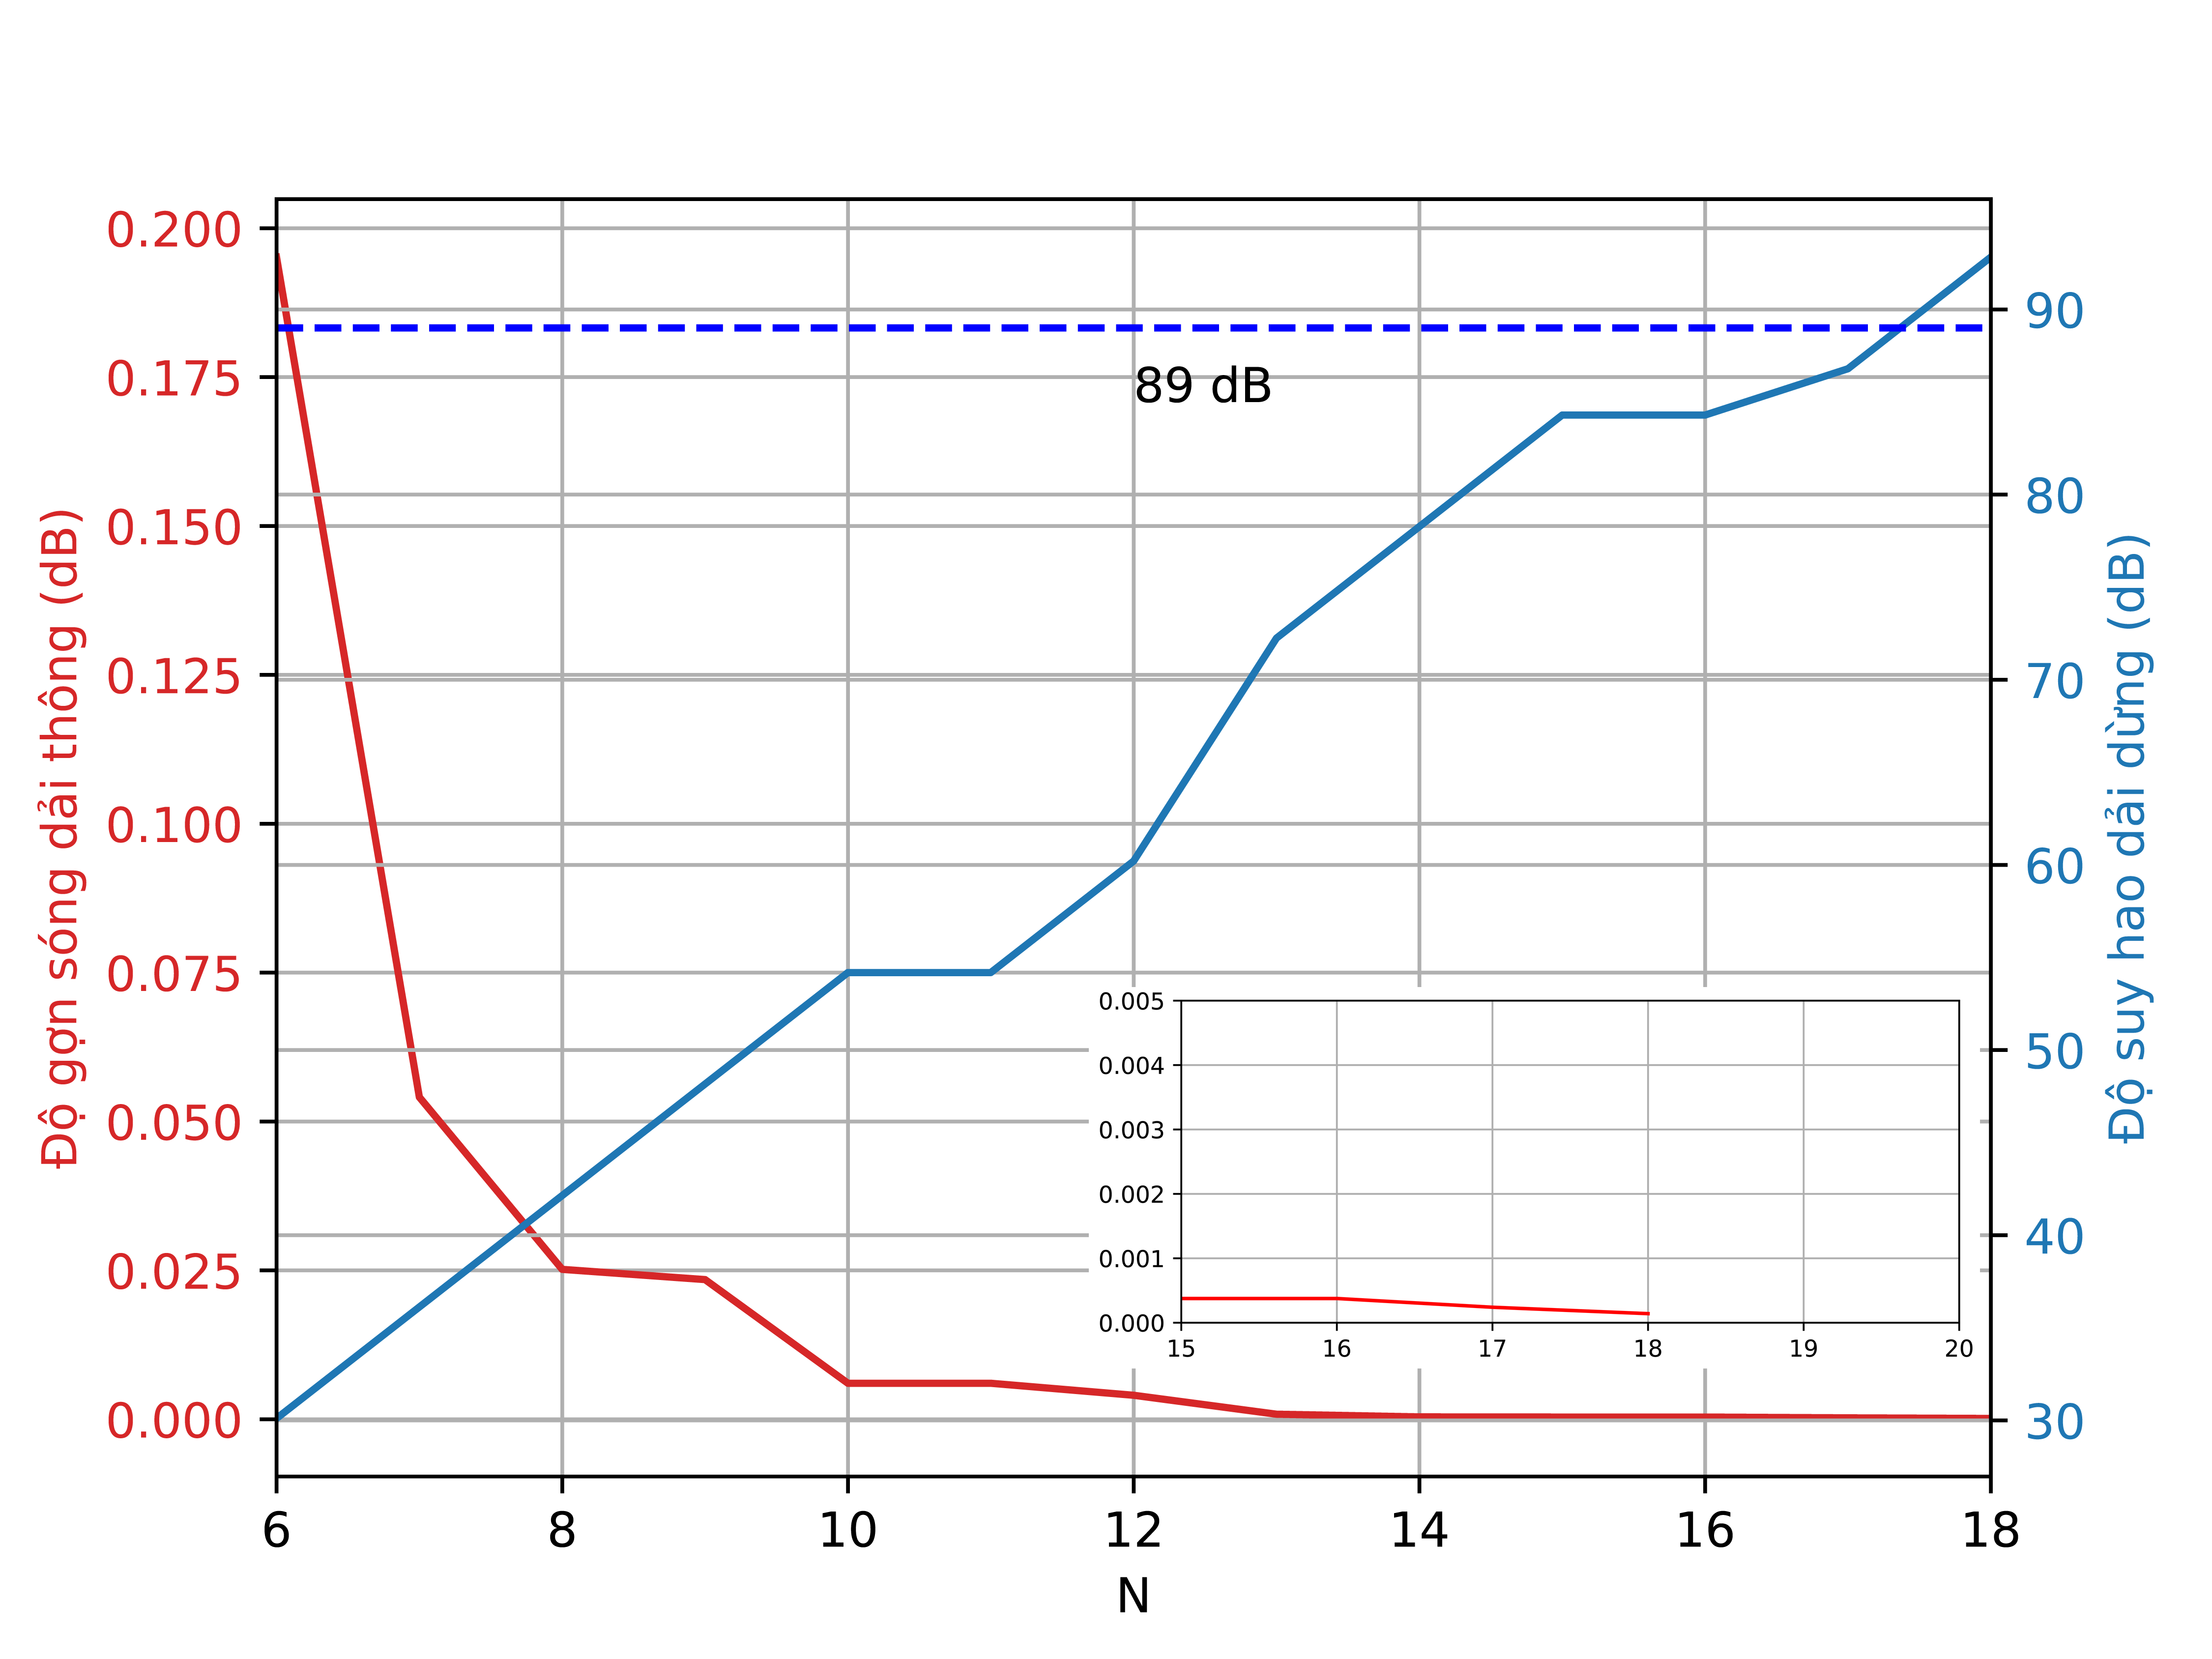
\includegraphics[width=11cm]{Images/Chuong4/plot/hb1.png}
    \caption[Độ suy hao dải dừng và độ gợn sóng của bộ lọc HB1 ứng với N khác nhau]{\bfseries \fontsize{12pt}{0pt}\selectfont Độ suy hao dải dừng và độ gợn sóng của bộ lọc HB1 ứng với N khác nhau}
    \label{hb111}
\end{figure}

\begin{figure}[H]
    \centering
    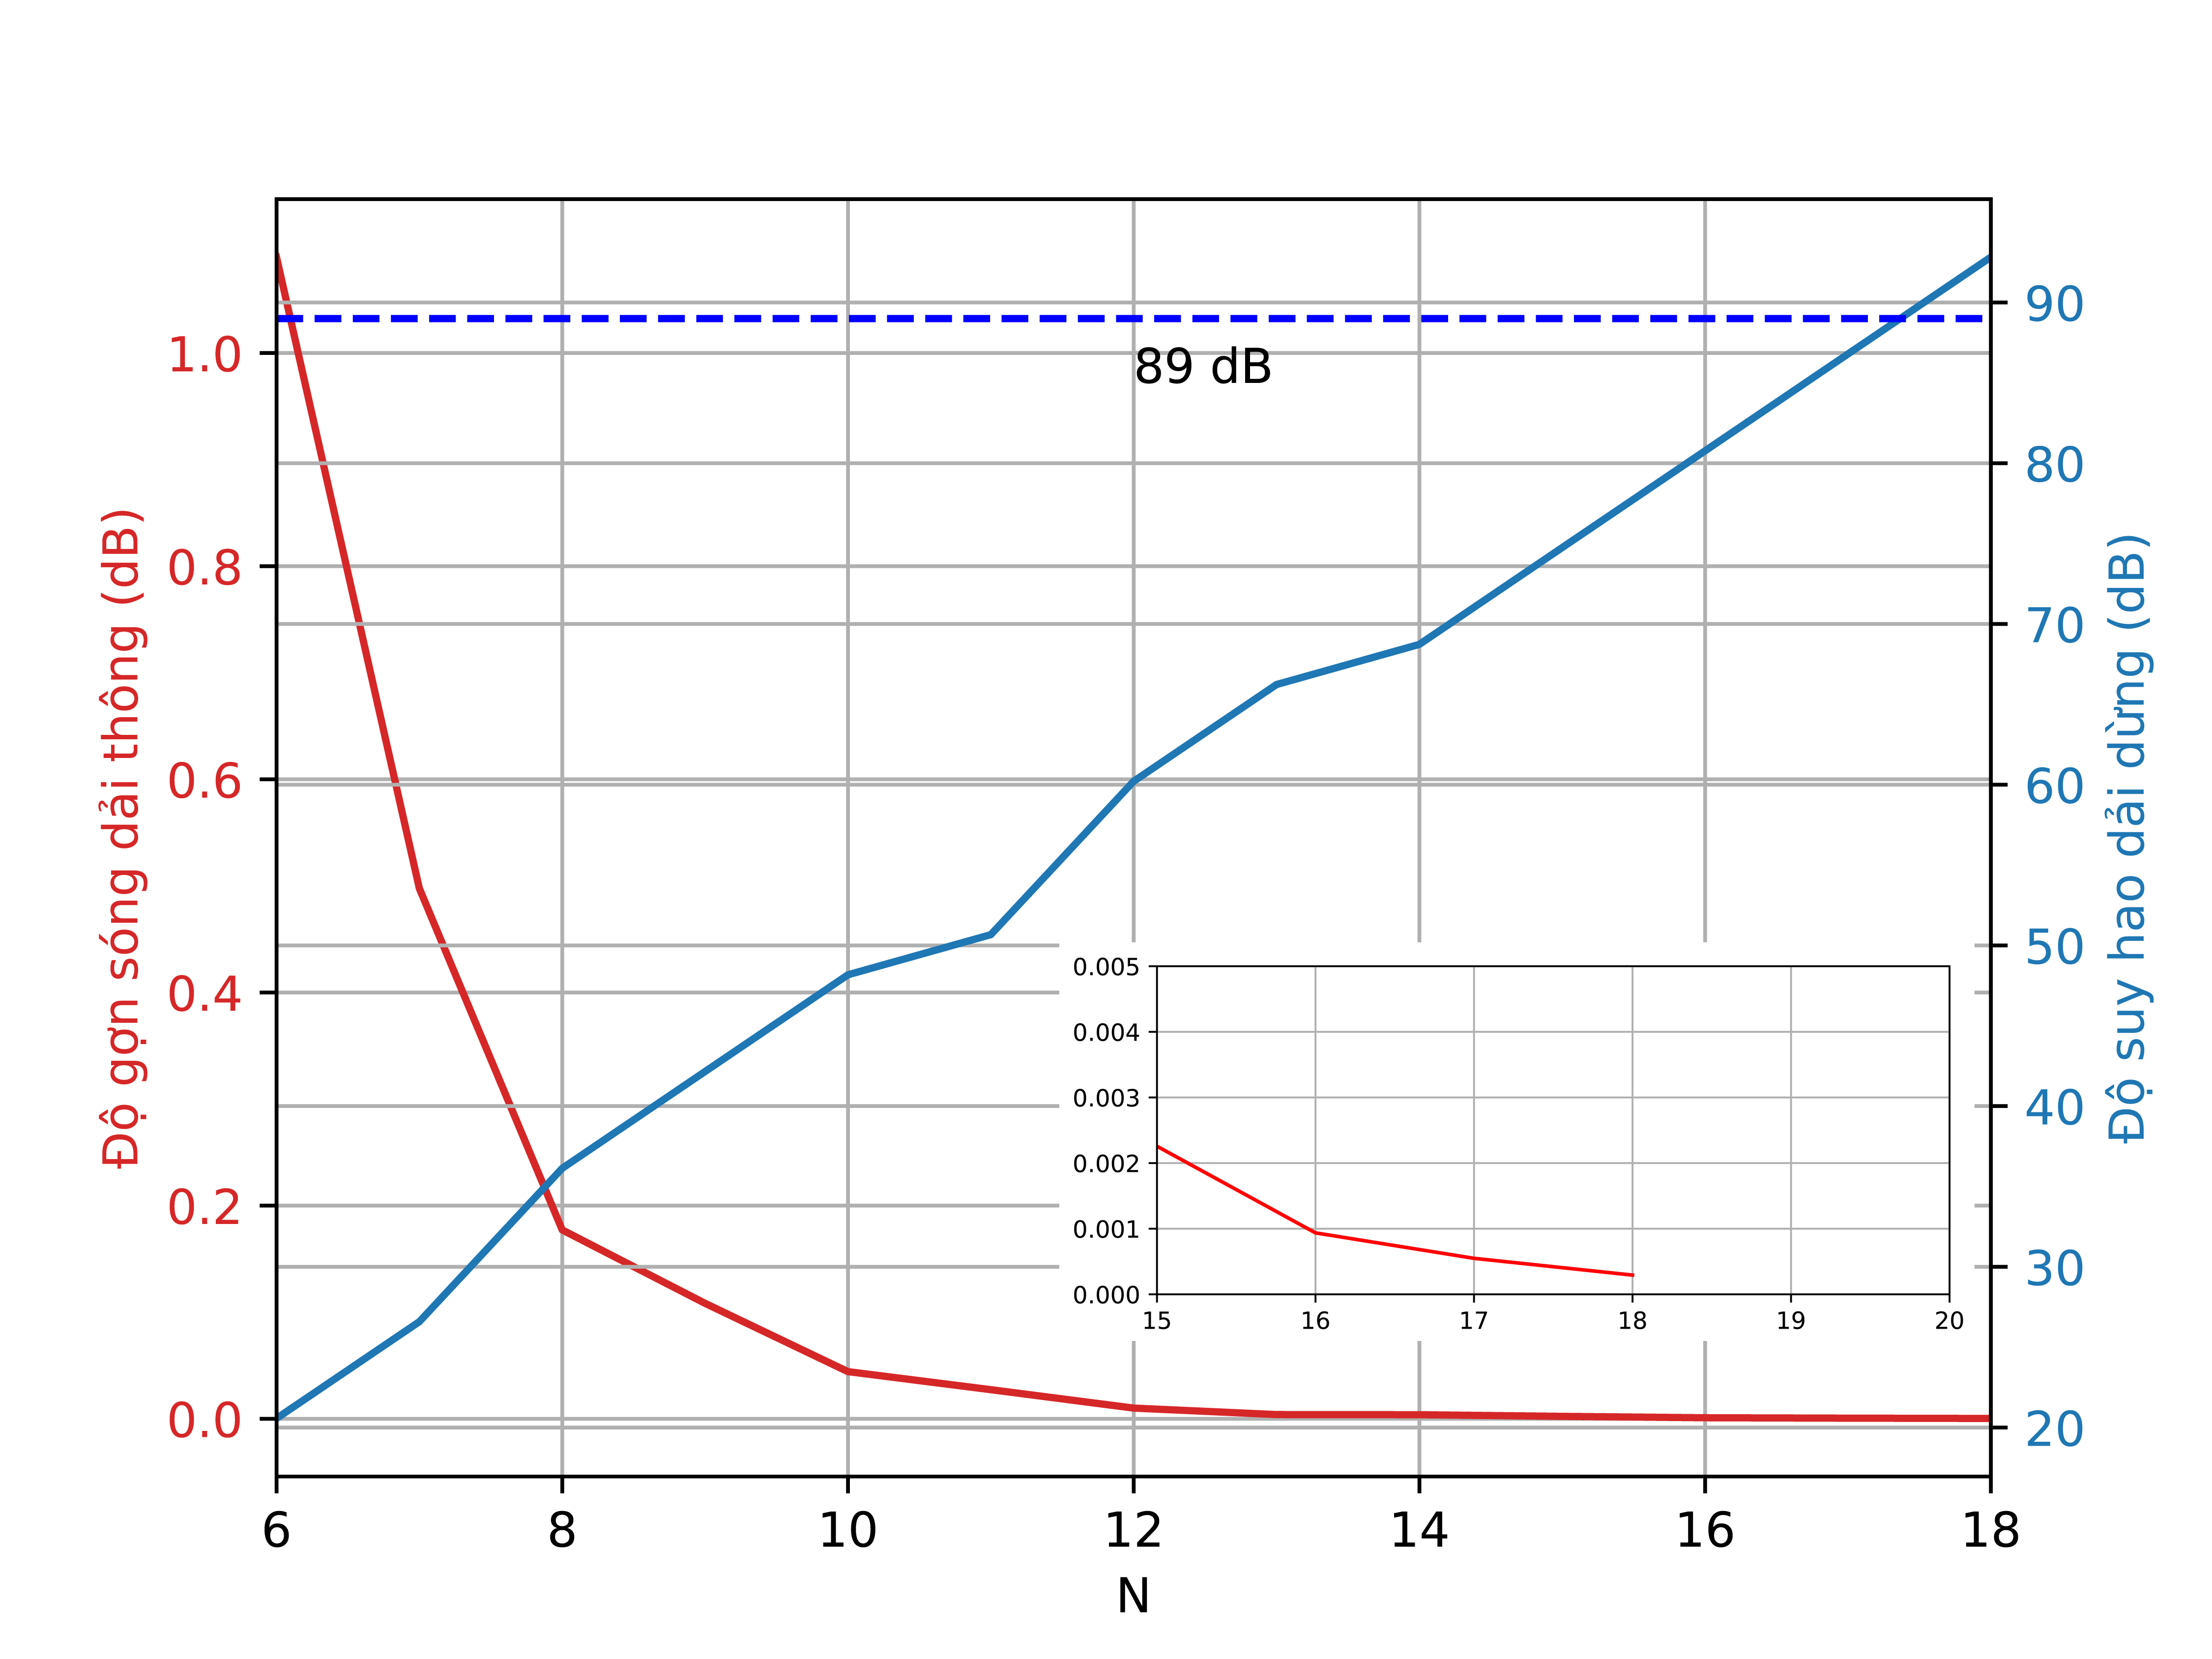
\includegraphics[width=11.5cm]{Images/Chuong4/plot/hb2.png}
    \caption[Độ suy hao dải dừng và độ gợn sóng của bộ lọc HB2 ứng với N khác nhau]{\bfseries \fontsize{12pt}{0pt}\selectfont Độ suy hao dải dừng và độ gợn sóng của bộ lọc HB2 ứng với các trường hợp N khác nhau}
    \label{hb222}
\end{figure}

\begin{figure}[H]
    \centering
    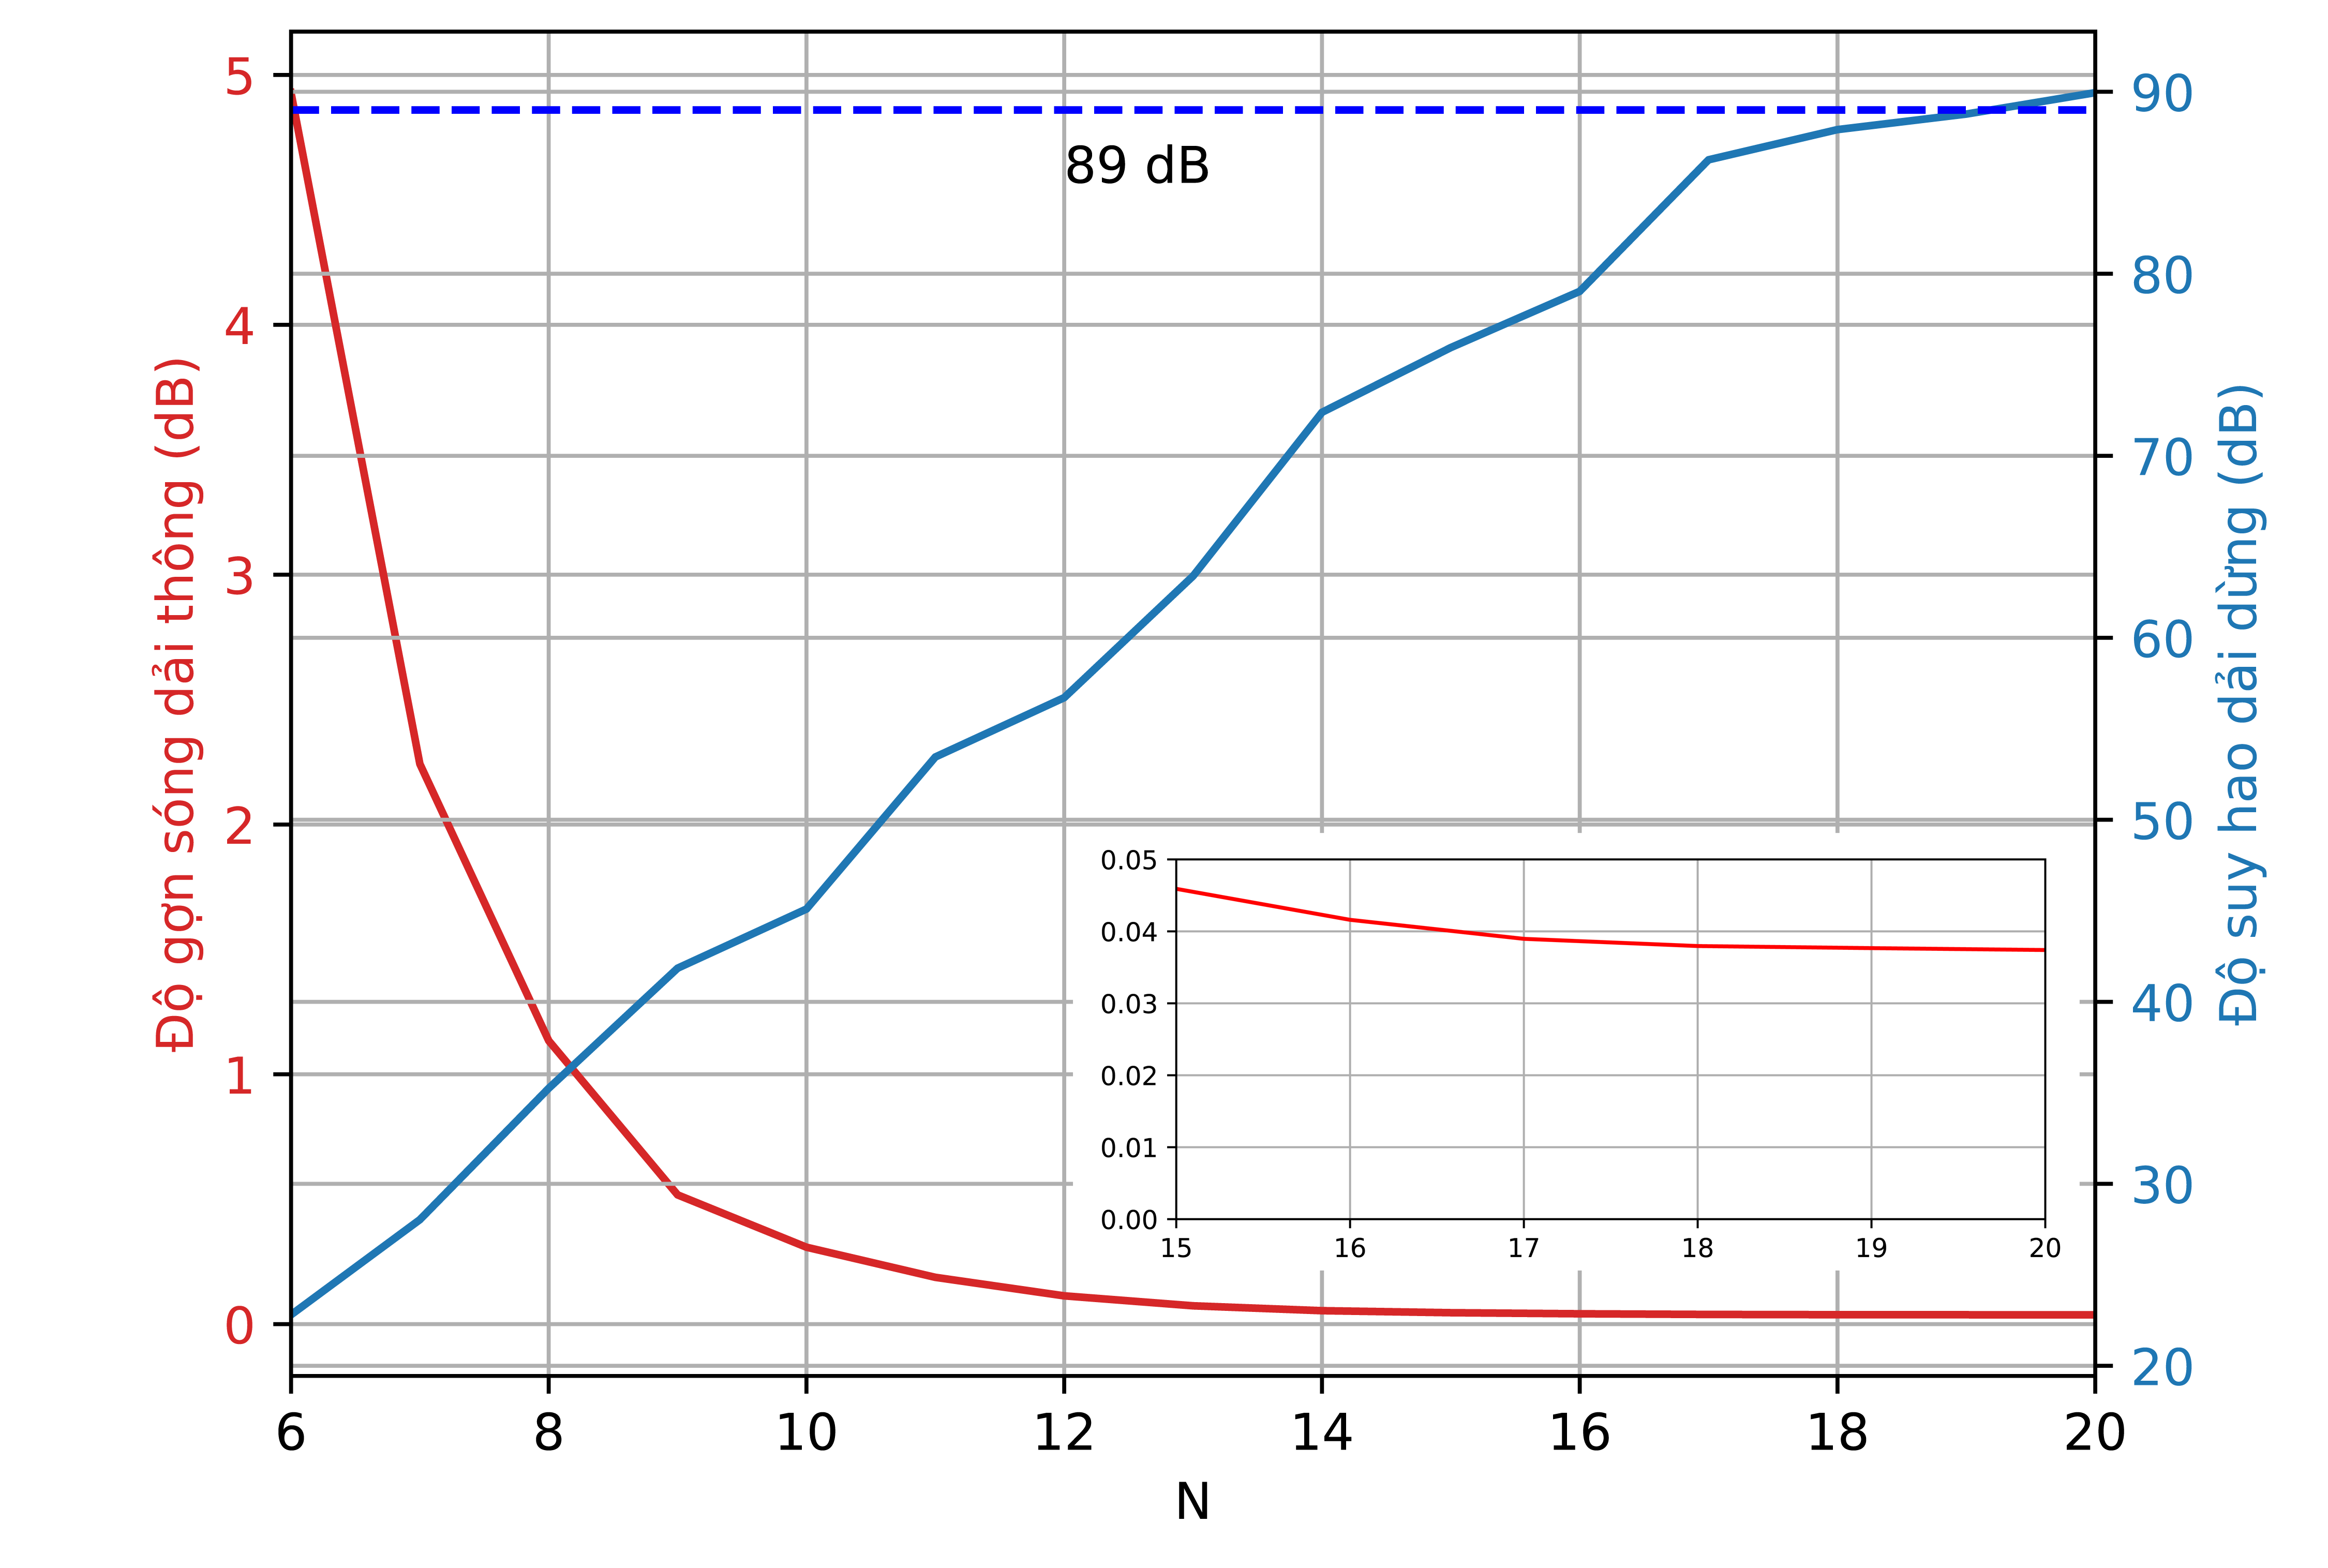
\includegraphics[width=11.5cm]{Images/Chuong4/plot/fir.png}
    \caption[Độ suy hao dải dừng và độ gợn sóng của bộ lọc FIR ứng với N khác nhau]{\bfseries \fontsize{12pt}{0pt}\selectfont Độ suy hao dải dừng và độ gợn sóng của bộ lọc FIR ứng với N khác nhau}
    \label{firrr}
\end{figure}
Từ đó, chúng ta có các biểu đồ mô tả độ suy hao dải dừng và độ gợn sóng trong từng trường hợp N khác nhau của từng bộ lọc lần lượt như hình \ref{hb111}, \ref{hb222}, \ref{firrr}. Nhận thấy với N bằng 18 thì 2 bộ lọc Half Band (1) và Half Band (2) đã đủ điều kiện. Tuy nhiên, đối với bộ lọc FIR thì N là 20, do vậy, chúng ta sẽ lấy chiều dài của toàn hệ thống là 20 để thuận tiện cho việc lưu trữ cũng như trích xuất các hệ số bộ lọc. Không những thế, khi tăng N thì hệ số của HB1 và HB2 sẽ dần tiệm cận với hệ số gốc hơn.
\begin{figure}[H]
    \centering
    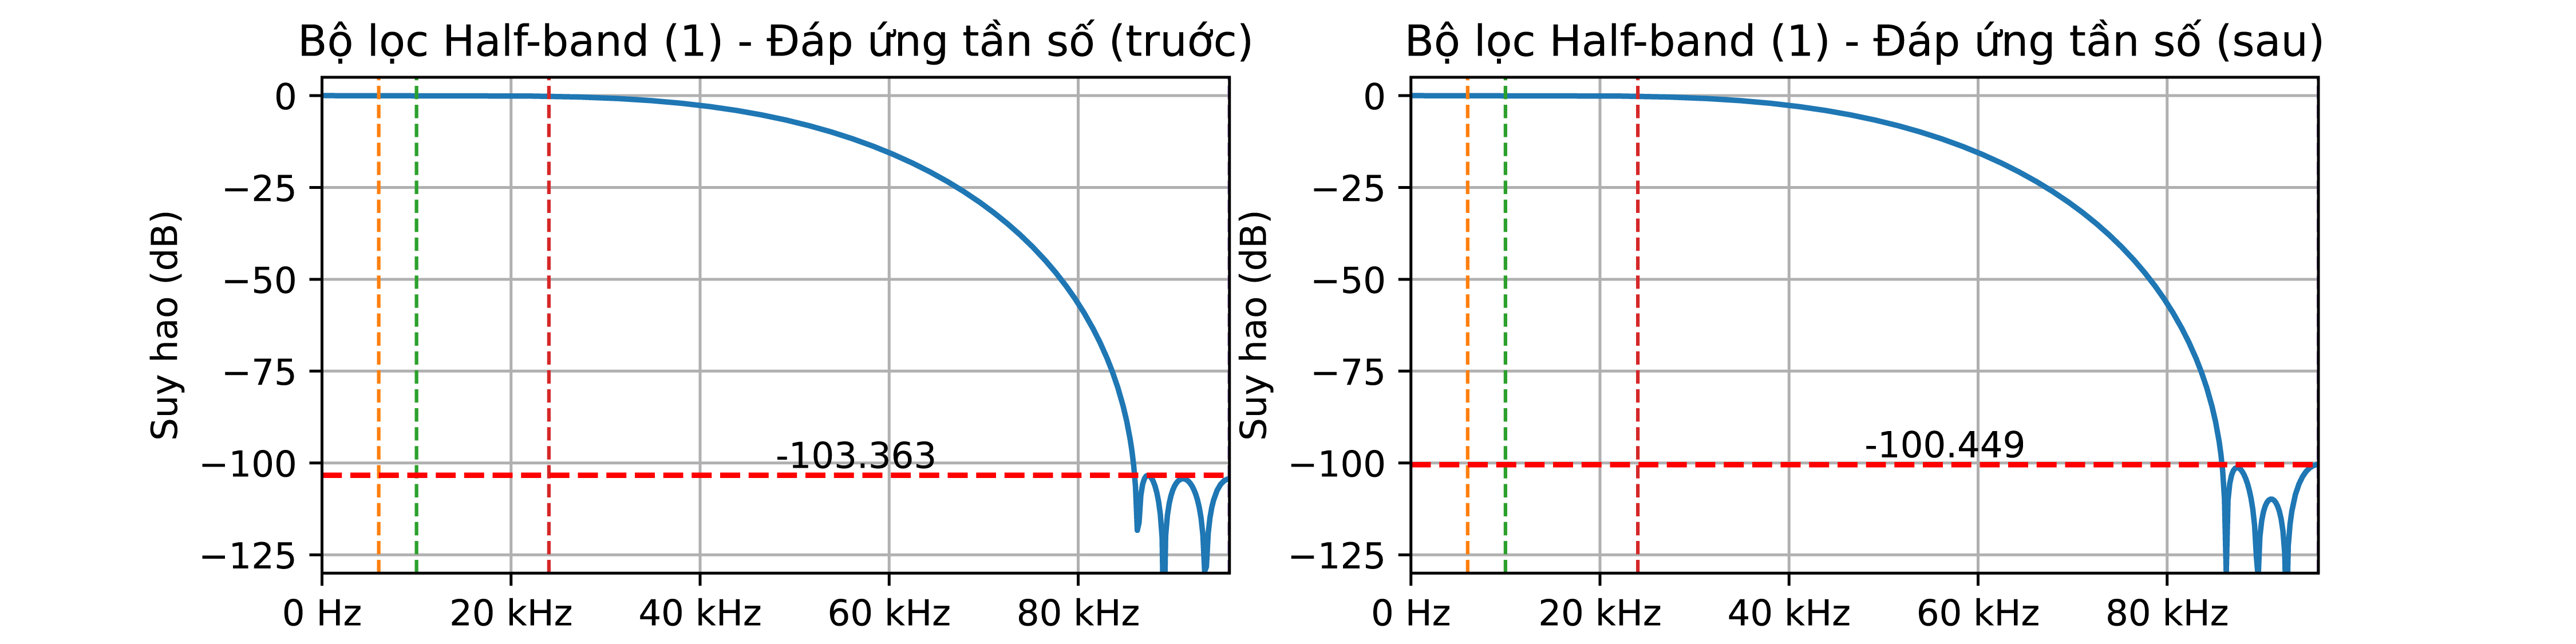
\includegraphics[width=17.5cm]{Images/Chuong4/hb1.png}
    \caption[Đáp ứng tần số của bộ lọc Half band (1) trước và sau khi sử dụng fixed-point]{\bfseries \fontsize{12pt}{0pt}\selectfont Đáp ứng tần số của bộ lọc Half band (1) trước và sau khi sử dụng fixed-point}
    \label{hb1_d}
\end{figure}

\begin{figure}[H]
    \centering
    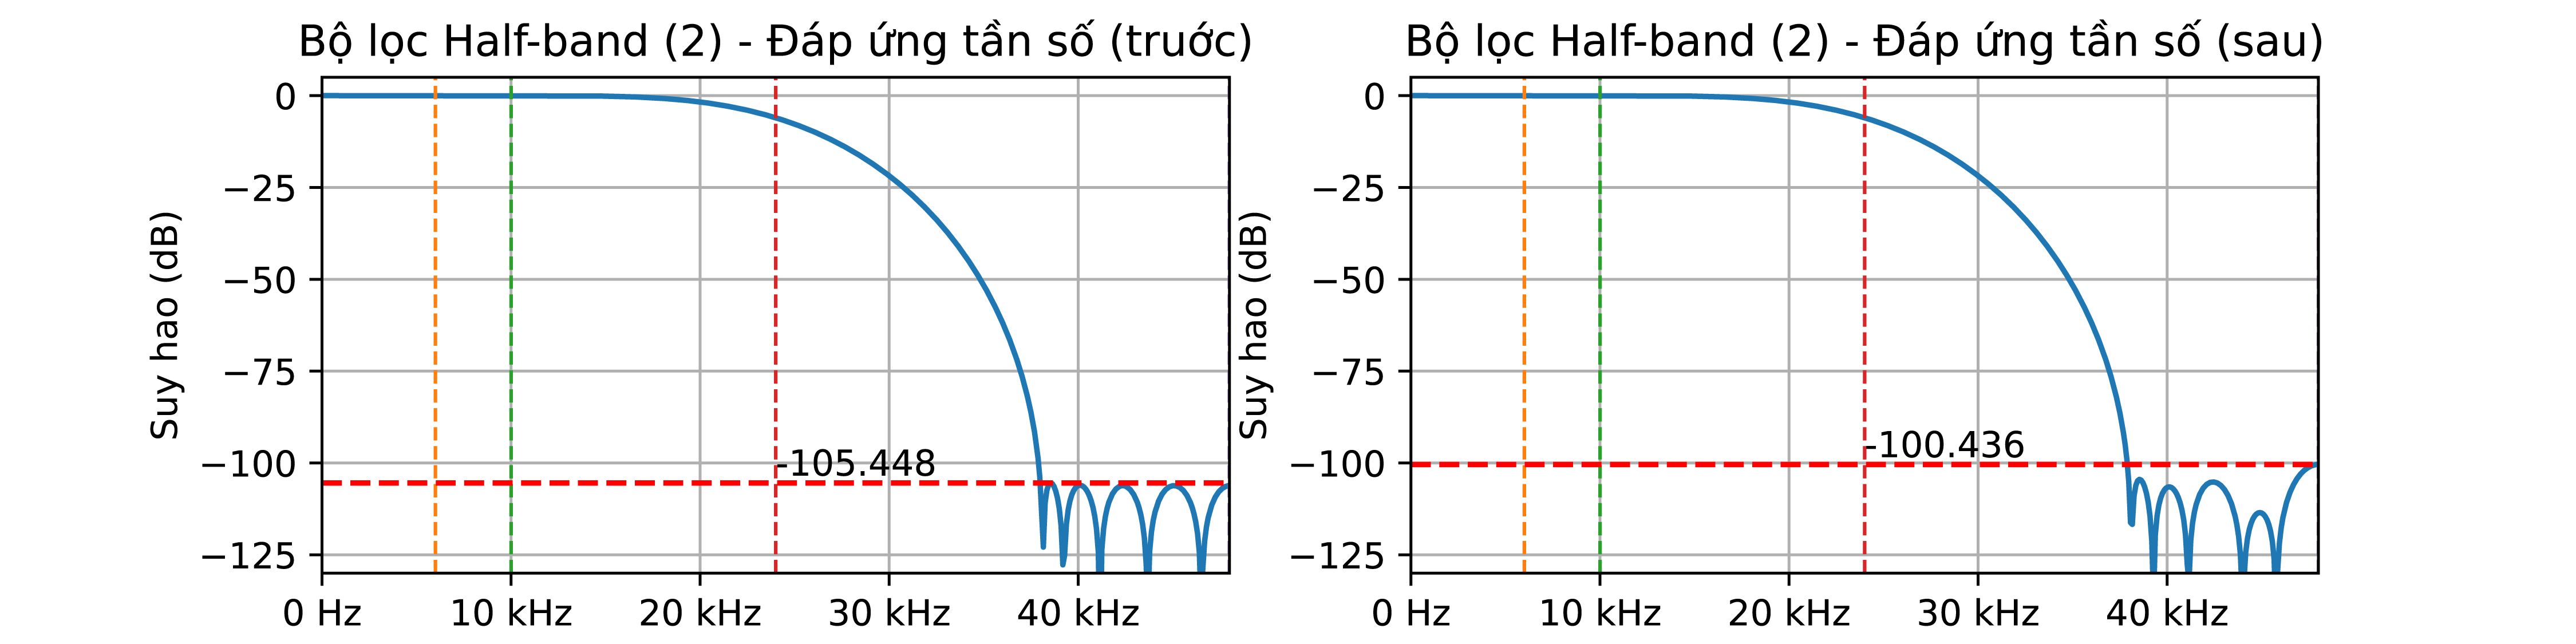
\includegraphics[width=17.5cm]{Images/Chuong4/hb2.png}
    \caption[Đáp ứng tần số của bộ lọc Half band (2) trước và sau khi sử dụng fixed-point]{\bfseries \fontsize{12pt}{0pt}\selectfont Đáp ứng tần số của bộ lọc Half band (2) trước và sau khi sử dụng fixed-point}
    \label{hb2_d}
\end{figure}
Chúng ta thu đáp ứng tần số của các bộ lọc sau khi quá trình fixed-point lần lượt như hình \ref{hb1_d}, \ref{hb2_d}, \ref{fir_d}.
\begin{figure}[H]
    \centering
    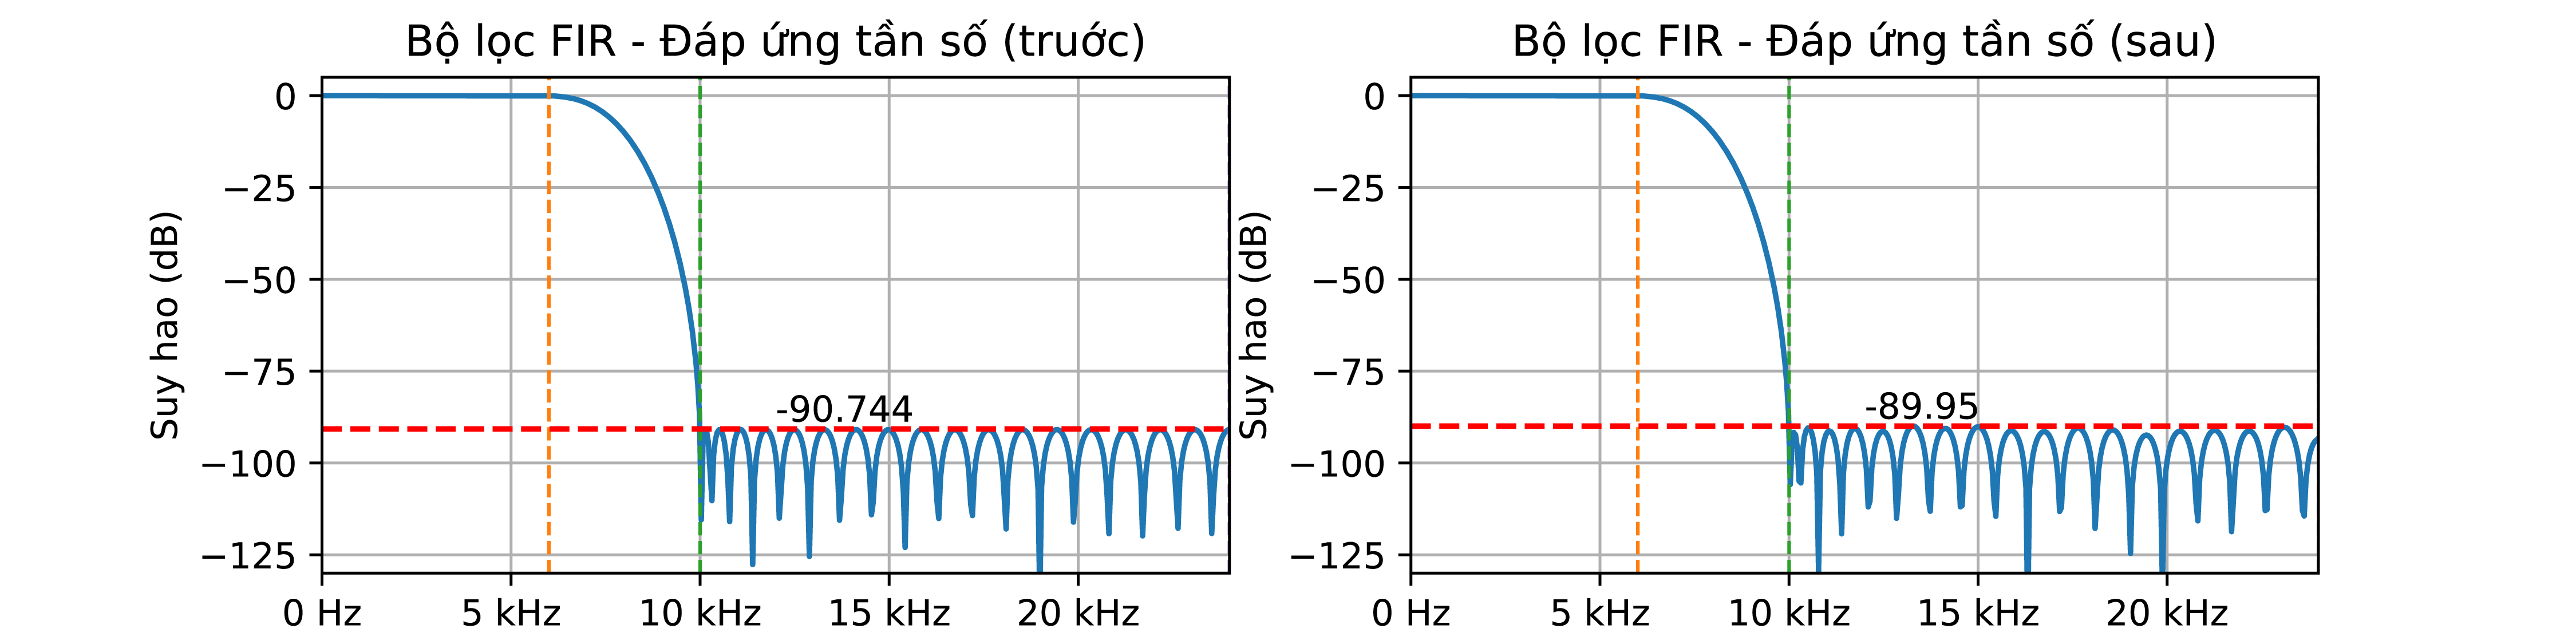
\includegraphics[width=17.5cm]{Images/Chuong4/fir.png}
    \caption[Đáp ứng tần số của bộ lọc FIR trước và sau khi sử dụng fixed-point]{\bfseries \fontsize{12pt}{0pt}\selectfont Đáp ứng tần số của bộ lọc FIR trước và sau khi sử dụng fixed-point}
    \label{fir_d}
\end{figure}



Theo quan sát, bộ lọc chỉ khác nhau lớn ở thông số suy giảm dải dừng, còn độ gợn sóng và các thông số còn lại không thay đổi. Độ suy giảm dải dừng giảm từ 0.794 dB đối với FIR, 3 và 5 dB với 2 bộ lọc còn lại, tuy nhiên độ suy giảm đó vẫn lớn hơn 89 dB (yêu cầu của hệ thống).

\textbf{Kết luận}: Chúng ta sẽ sử dụng tất cả hệ số nhân với $2^{20}$ để ép thành số nguyên (hệ thập phân).
\subsubsection{Mô tả chung}
Bộ chuyển đổi PDM sang PCM nhiều giai đoạn sử dụng Decimation (dti\_pdm2pcm) chuyển đổi dữ liệu PDM 1 bit với tốc lấy mẫu cao thành dữ liệu PCM với  tốc độc lấy mẫu thấp hơn. Tần số cấp cho bộ gấp 4 lần tần số lấy mẫu của PDM, từ tần số này sẽ cấp và chia tần ra các tần số cần thiết cho dti\_pdm2pcm. Tín hiệu PCM đầu ra sẽ đi kèm theo sườn dương của tín hiệu đồng hồ PCM đầu ra với độ rộng bit do người dùng quyết định (thường là 24 bit), độ rộng càng lớn thì chất lượng âm thanh đầu ra càng cao. Sơ đồ chân của dti\_pdm2pcm được mô tả như hình \ref{top_pdm2pcm}.

\begin{figure}[H]
    \centering
    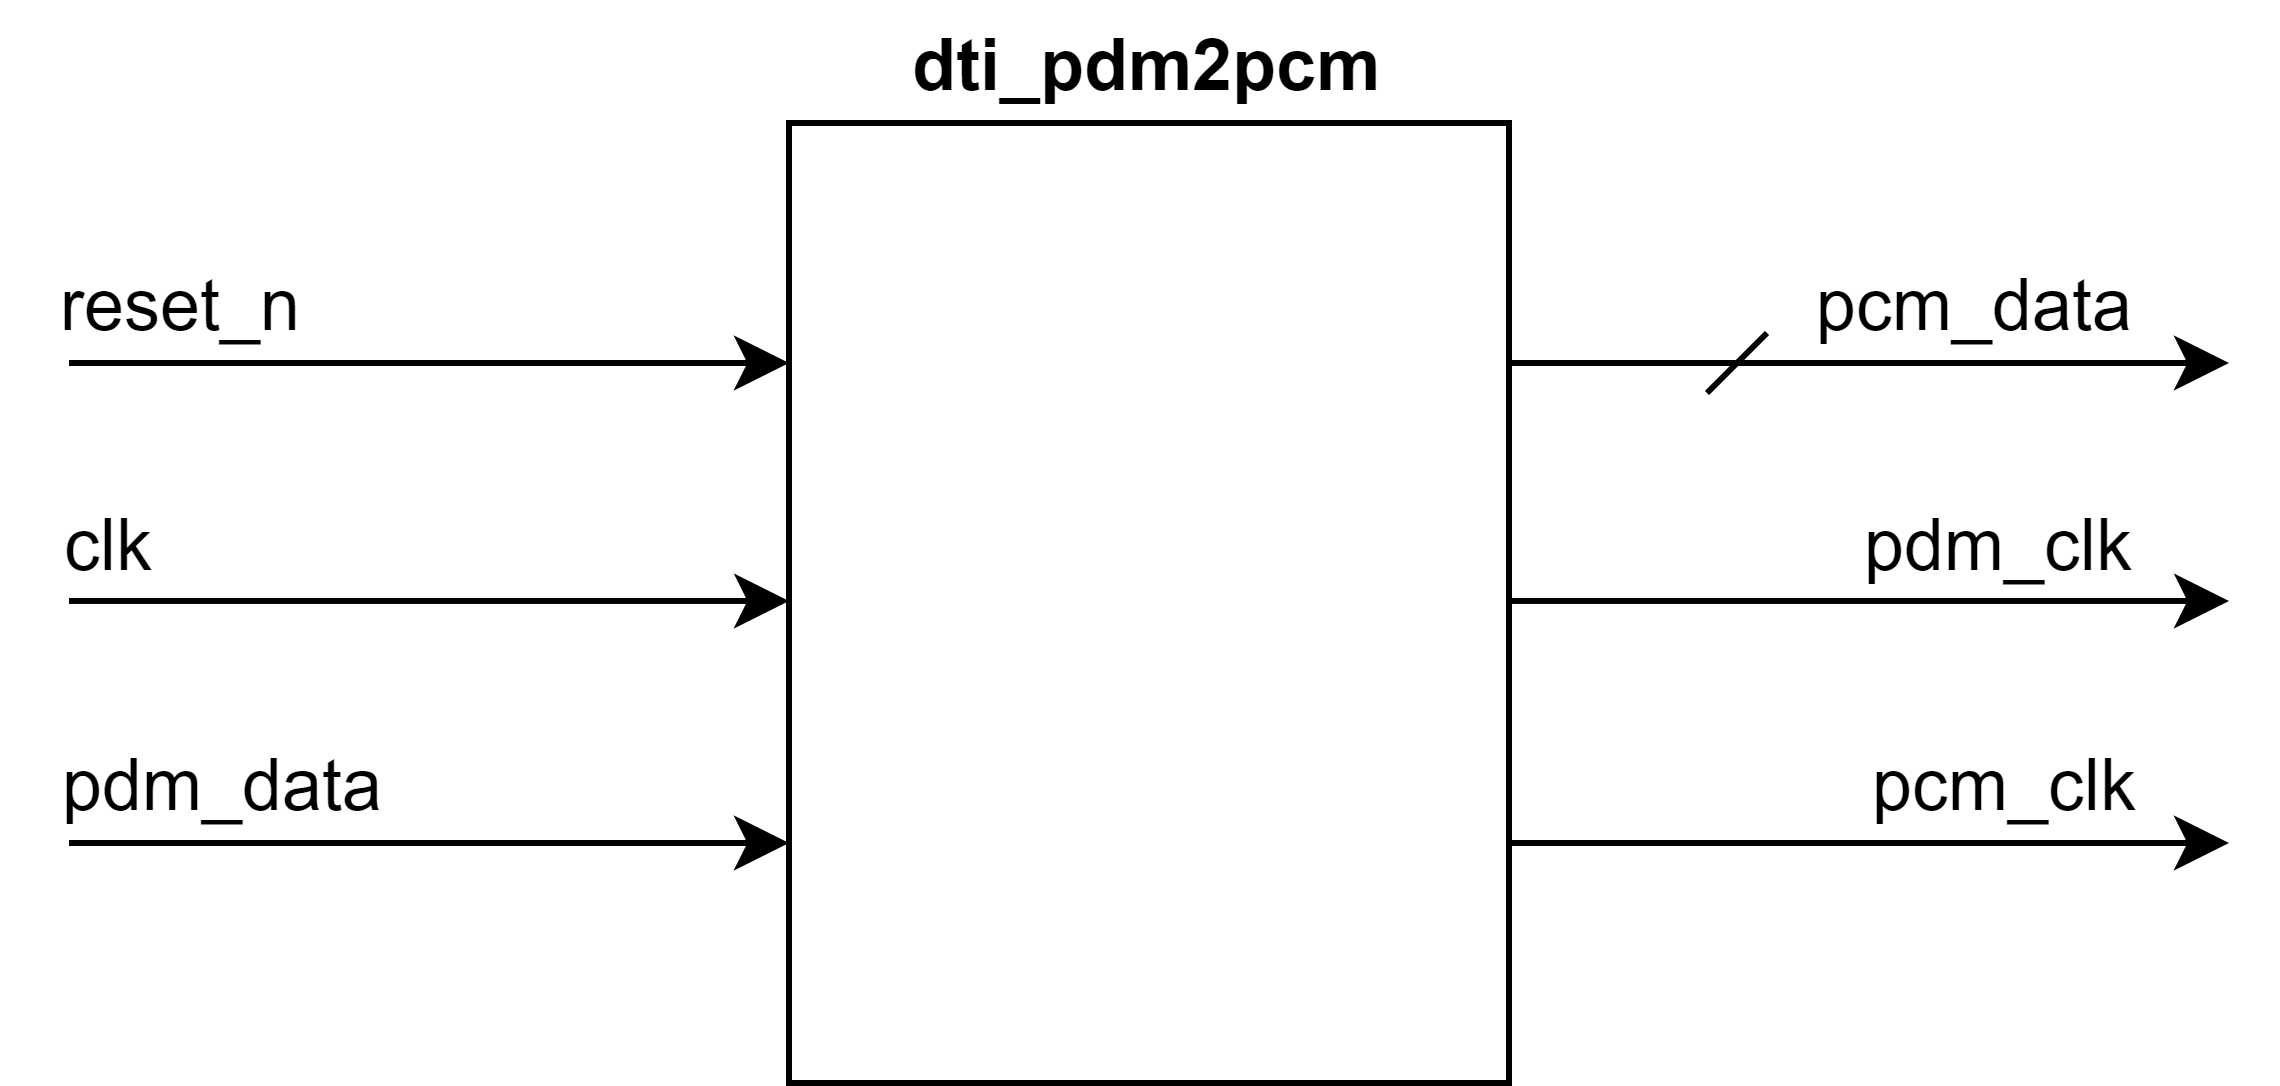
\includegraphics[width=9.5cm]{Images/Chuong4/top.png}
    \caption[Sơ đồ tổng quát của bộ PCM2PDM]{\bfseries \fontsize{12pt}{0pt}\selectfont Sơ đồ tổng quát của bộ PCM2PDM}
    \label{top_pdm2pcm}
\end{figure}
Các chân của bộ chuyển đổi sẽ được trình bày chi tiết ở bảng \ref{top_signal}. Bảng \ref{hangso} mô tả các hằng số được sử dụng trong thiết kế.

\begin{table}[H]
    \centering
    \caption[Mô tả chân vào ra của hệ thống]{\bfseries\fontsize{12pt}{0pt}\selectfont Mô tả chân vào ra của hệ thống}
\begin{tabular}{|c|c|c|l|}
\hline
\textbf{Tên chân} & \textbf{Vào/ ra} & \textbf{Độ rộng bit} & \multicolumn{1}{c|}{\textbf{Mô tả chức năng}}                                               \\ \hline
clk       & vào & 1          & Clock đồng bộ hoạt động của hệ thống \\ \hline
reset\_n          & vào              & 1                    & \begin{tabular}[c]{@{}l@{}}Chân reset không đồng bộ, tích cực mức\\ thấp\end{tabular}       \\ \hline
pdm\_data & vào & 1          & Dữ liệu từ MEMS, dạng PDM            \\ \hline
pdm\_clk  & ra  & 1          & Clock lấy mẫu của dữ liệu PDM        \\ \hline
pcm\_data & ra  & PCM\_WIDTH & Dữ liệu PCM sau khi được chuyển đổi  \\ \hline
pcm\_clk          & ra               & 1                    & \begin{tabular}[c]{@{}l@{}}Clock đi cùng dữ liệu PCM, dùng cho thiết\\ bị khác\end{tabular} \\ \hline
\end{tabular}
    \label{top_signal}
\end{table}

Điều đặc biệt của thiết kế là các tham số của các bộ lọc sẽ được sinh ra từ các tính toán trên phần mềm sử dụng \textbf{Python}. Đồng nghĩa với việc, chúng ta chỉ cần điền các thông số yêu cầu ví dụ như \textbf{Dải thông}, \textbf{Dải dừng}, \textbf{Độ suy hao dải dừng}, \textbf{Độ gợn sóng của dải thông} vào phần mềm. Nó sẽ tự động tính toán và nạp các hệ số bộ lọc, tối ưu các độ rộng bit của mỗi sau bộ lọc và sau đó sẽ nạp vào RTL code. Từ đây, chúng ta có thể thiết kế bộ lọc cho bất kỳ thiết bị microphone nào. Ở trong thiết kế này, chúng ta sẽ chỉ tập trung và tối ưu thiết kế cho thiết bị \textbf{MP34DT01-M}.


\begin{table}[H]
    \centering
    \caption[Hằng số thiết kế]{\bfseries\fontsize{12pt}{0pt}\selectfont Hằng số thiết kế}
\begin{tabular}{|l|c|l|}
\hline
\multicolumn{1}{|c|}{\textbf{Hằng số}} & \textbf{Giá trị} & \multicolumn{1}{c|}{\textbf{Mô tả}} \\ \hline
PCM\_WIDTH  & 24 & Độ rộng của tín hiệu PCM đầu ra \\ \hline
MULP\_WIDTH & 21 & Kích thước đầu vào của bộ nhân  \\ \hline
FIR\_SIZE   & 51 & Số lượng taps của bộ lọc FIR    \\ \hline
HB1\_SIZE   & 11 & Số lượng taps của bộ lọc HB1    \\ \hline
HB2\_SIZE   & 19 & Số lượng taps của bộ lọc HB2    \\ \hline
\end{tabular}
    \label{hangso}
\end{table}
\subsubsection{Kiến trúc}
Sơ đồ tổng quan của kiến trúc được mô tả như hình \ref{arc_top}.
\begin{figure}[H]
    \centering
    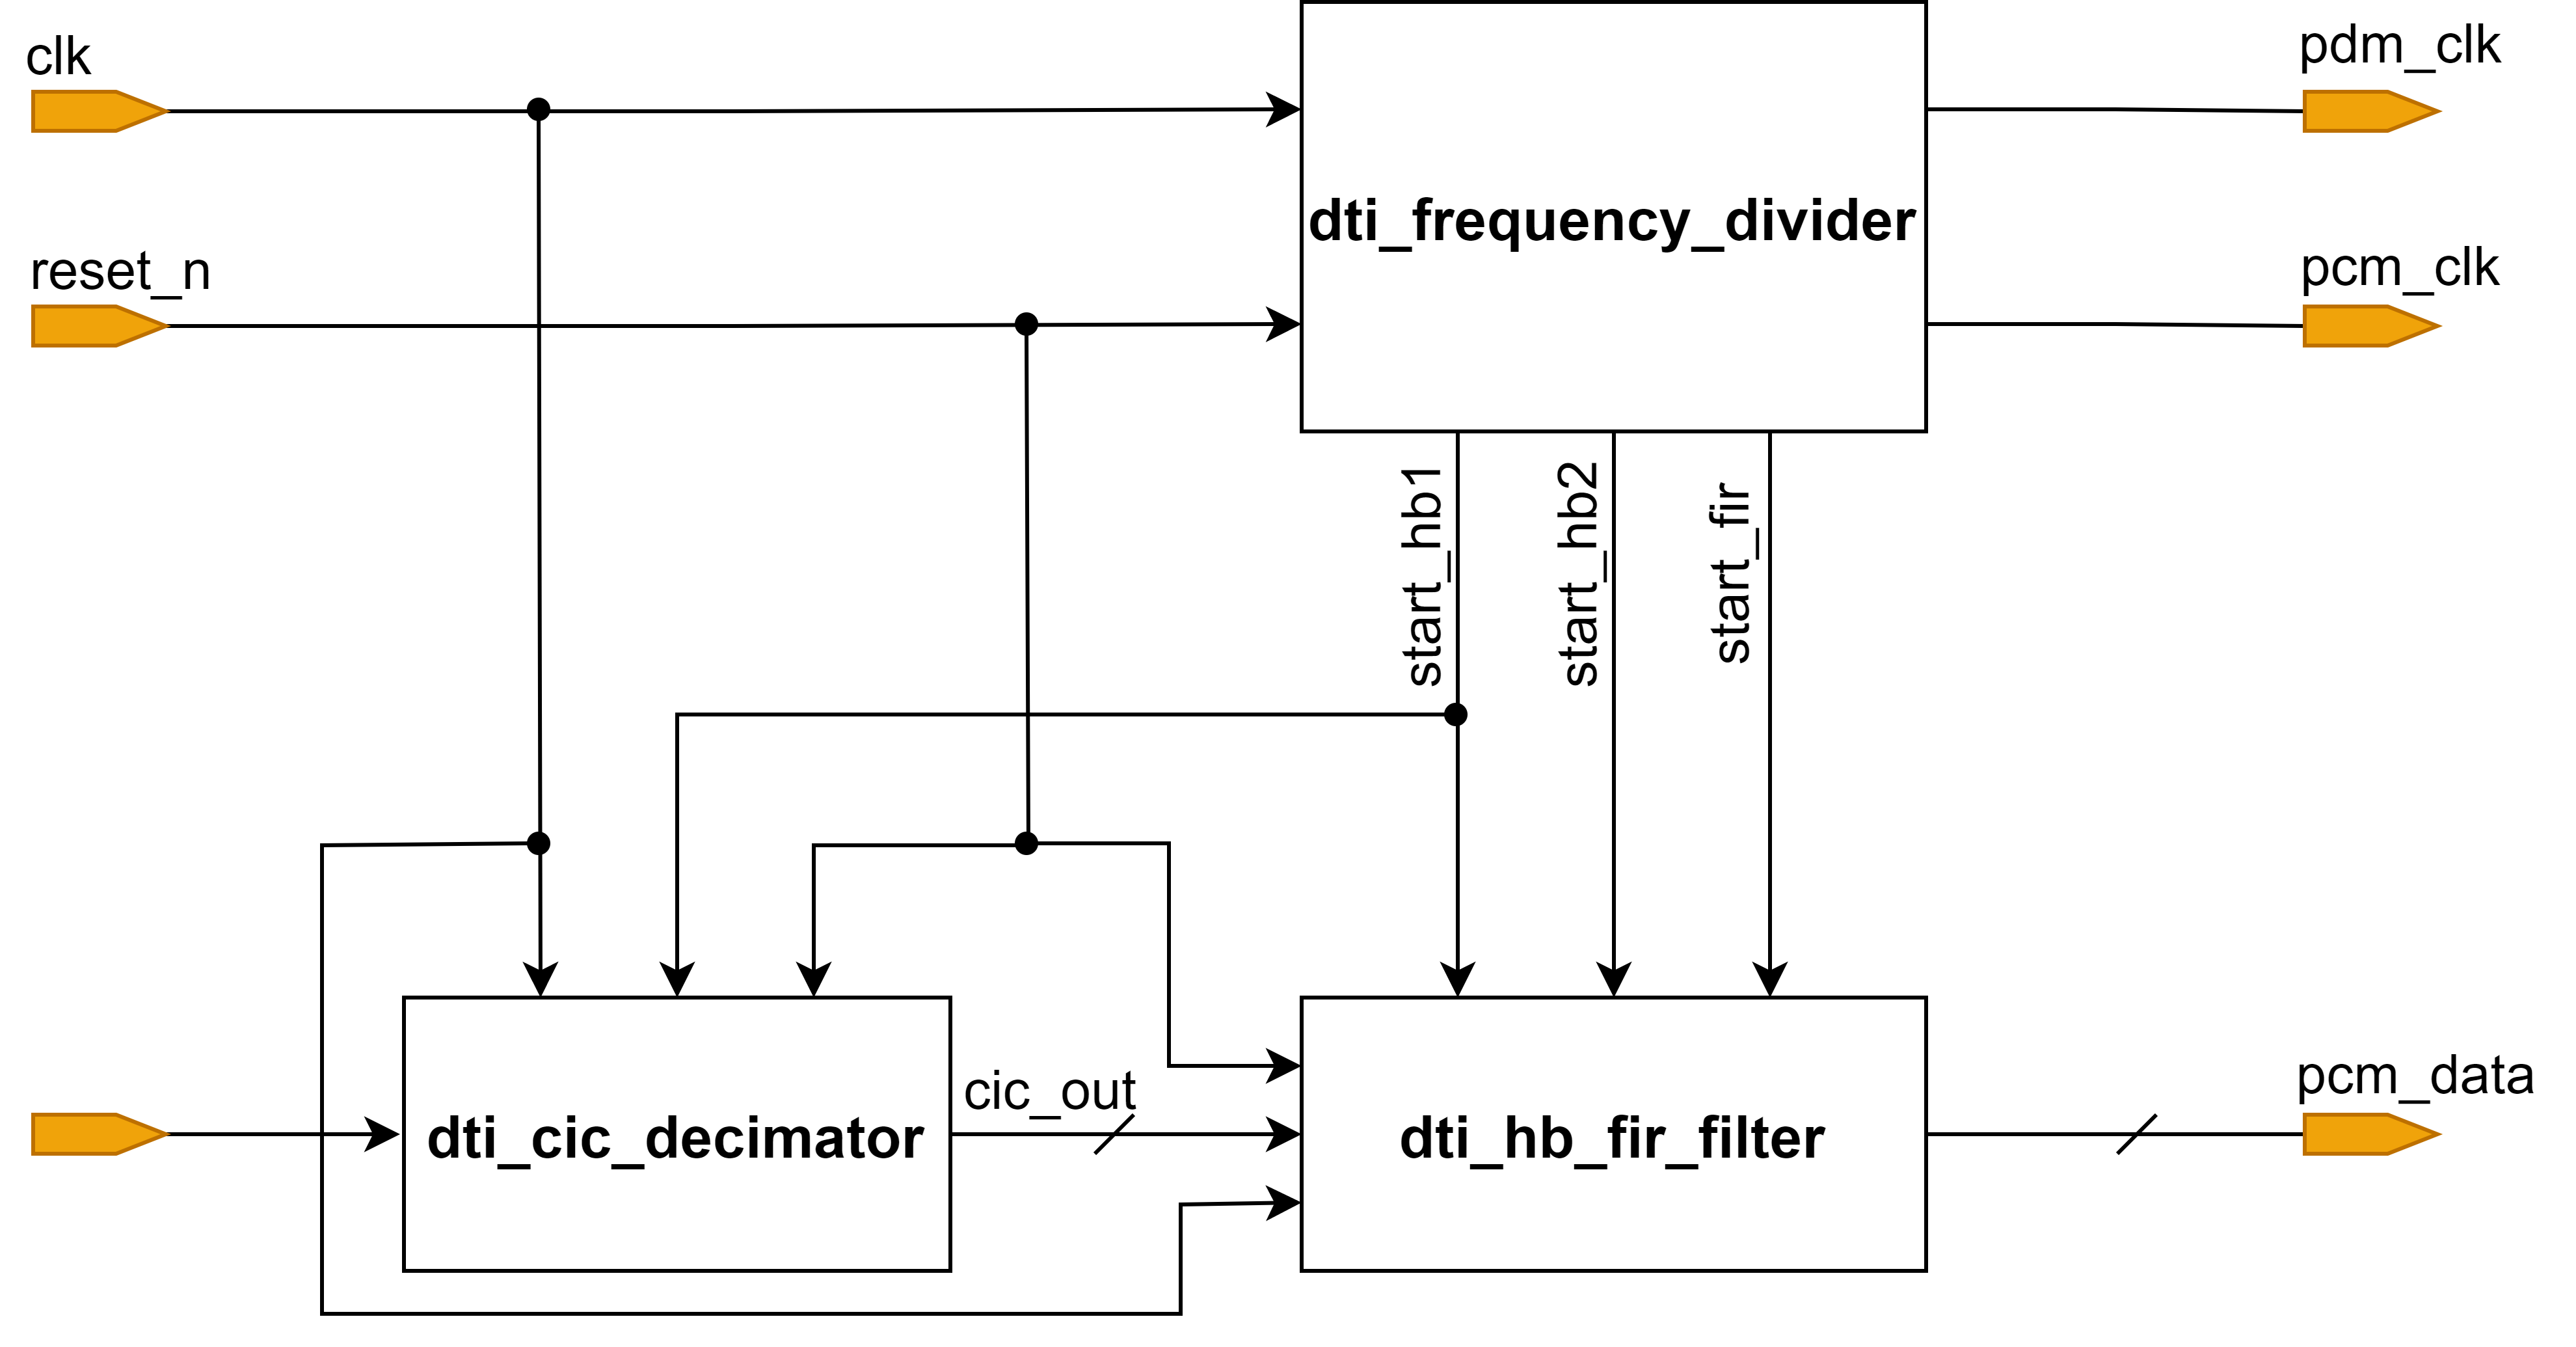
\includegraphics[width=12cm]{Images/Chuong4/arc_top.png}
    \caption[Kiến trúc của bộ PCM2PDM]{\bfseries \fontsize{12pt}{0pt}\selectfont Kiến trúc của bộ PCM2PDM}
    \label{arc_top}
\end{figure}

Chức năng của từng khối :
\begin{itemize}
    \item \textbf{dti\_frequency\_divider} đóng vai trò là bộ điều khiển, nó tạo ra tín hiệu điều khiển để khởi động hoạt động của các thành phần bên trong khối khác. Nó hoạt động như bộ chia tần.
    \item \textbf{dti\_cic\_decimator} là một bộ lọc CIC với hệ số decimation 12x và 4 tầng.
    \item \textbf{dti\_hb\_fir\_filter} là một nhóm gồm 2 bộ lọc Half Band và 1 bộ lọc FIR với tổng hệ số Decimation là 4. Vai trò của chúng là lấy mẫu xuống và bù tín hiệu.
\end{itemize}

\subsubsection{Thiết kế chi tiết từng khối}
\paragraph{dti\_frequency\_divider}
\textbf{dti\_frequency\_divider} có chức năng chia tần số từ clock đầu vào thành clock có tần số bé hơn với tỷ lệ DECIMATION là tỷ lệ chia tần. Đồng thời tạo ra tín hiệu báo hiệu quá trình đổi tần.

Sơ đồ chân vào ra của khối được mô tả ở hình \ref{frequency}.

\begin{figure}[H]
    \centering
    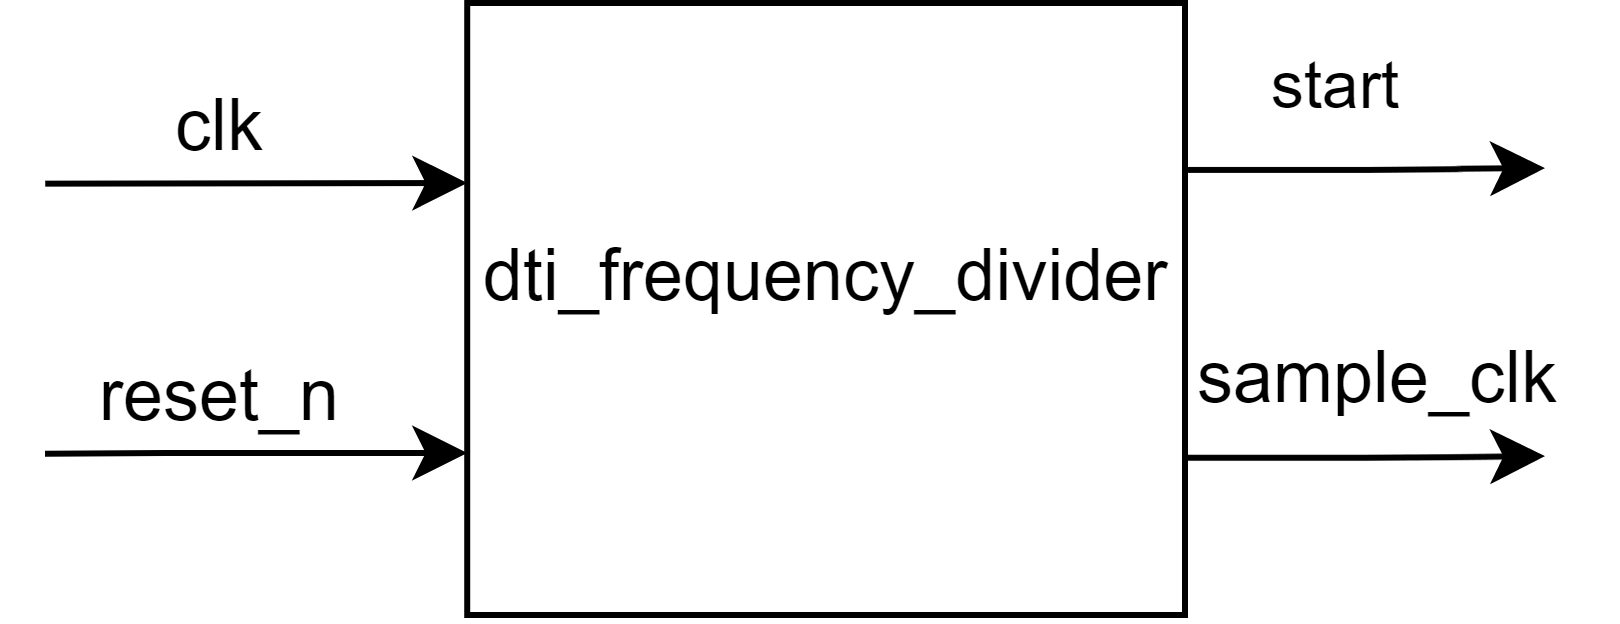
\includegraphics[width=7.5cm]{Images/Chuong4/frequency/frequency.png}
    \caption[Sơ đồ khối của dti\_frequency\_divider]{\bfseries \fontsize{12pt}{0pt}\selectfont Sơ đồ khối của dti\_frequency\_divider}
    \label{frequency}
\end{figure}
Bảng \ref{frequency_t} mô tả các chân vào ra của khối.
\begin{table}[H]
    \centering
    \caption[Mô tả chân vào ra của dti\_frequency\_divider]{\bfseries\fontsize{12pt}{0pt}\selectfont Mô tả chân vào ra của dti\_frequency\_divider}
    \begin{tabular}{|l|c|c|l|}
\hline
\multicolumn{1}{|c|}{\textbf{Tên chân}} &
  \textbf{Vào/ ra} &
  \textbf{Độ rộng bit} &
  \multicolumn{1}{c|}{\textbf{Mô tả chức năng}} \\ \hline
clk         & vào & 1 & Clock đồng bộ hoạt động của hệ thống \\ \hline
reset\_n &
  vào &
  1 &
  \begin{tabular}[c]{@{}l@{}}Chân reset không đồng bộ, tích cực mức\\ thấp\end{tabular} \\ \hline
start &
  ra &
  1 &
  \begin{tabular}[c]{@{}l@{}}Tín hiệu điều khiển, cho biết dữ liệu đầu \\ vào bộ lọc đã sẵn sàng\end{tabular} \\ \hline
sample\_clk & ra  & 1 & Clock đã được hạ tần                 \\ \hline
\end{tabular}
    \label{frequency_t}
\end{table}
Kiến trúc của khối được mô tả ở hình \ref{frequency_a}, quá trình hoạt động tương ứng được biểu diễn như hình \ref{frequency_tt}, bộ đếm thực hiện đếm bắt đầu đếm từ giá trị 0, đến nửa DECIMITION là đổi chiều giá trị của sample\_clk đồng nghĩa với việc tạo ra clock với độ lớn nhỏ hơn DECIMTION với tần số vào. Ở giá trị bộ đếm bằng 0, tín hiệu start được kích hoạt.
\begin{figure}[H]
    \centering
    
\includegraphics[width=13.5cm]{Images/Chuong4/frequency/frequency_timing.png}
    \caption[Biểu đồ thời gian của dti\_frequency\_divider]{\bfseries \fontsize{12pt}{0pt}\selectfont Biểu đồ thời gian của dti\_frequency\_divider}
    \label{frequency_tt}
\end{figure}



\begin{figure}[H]
    \centering
    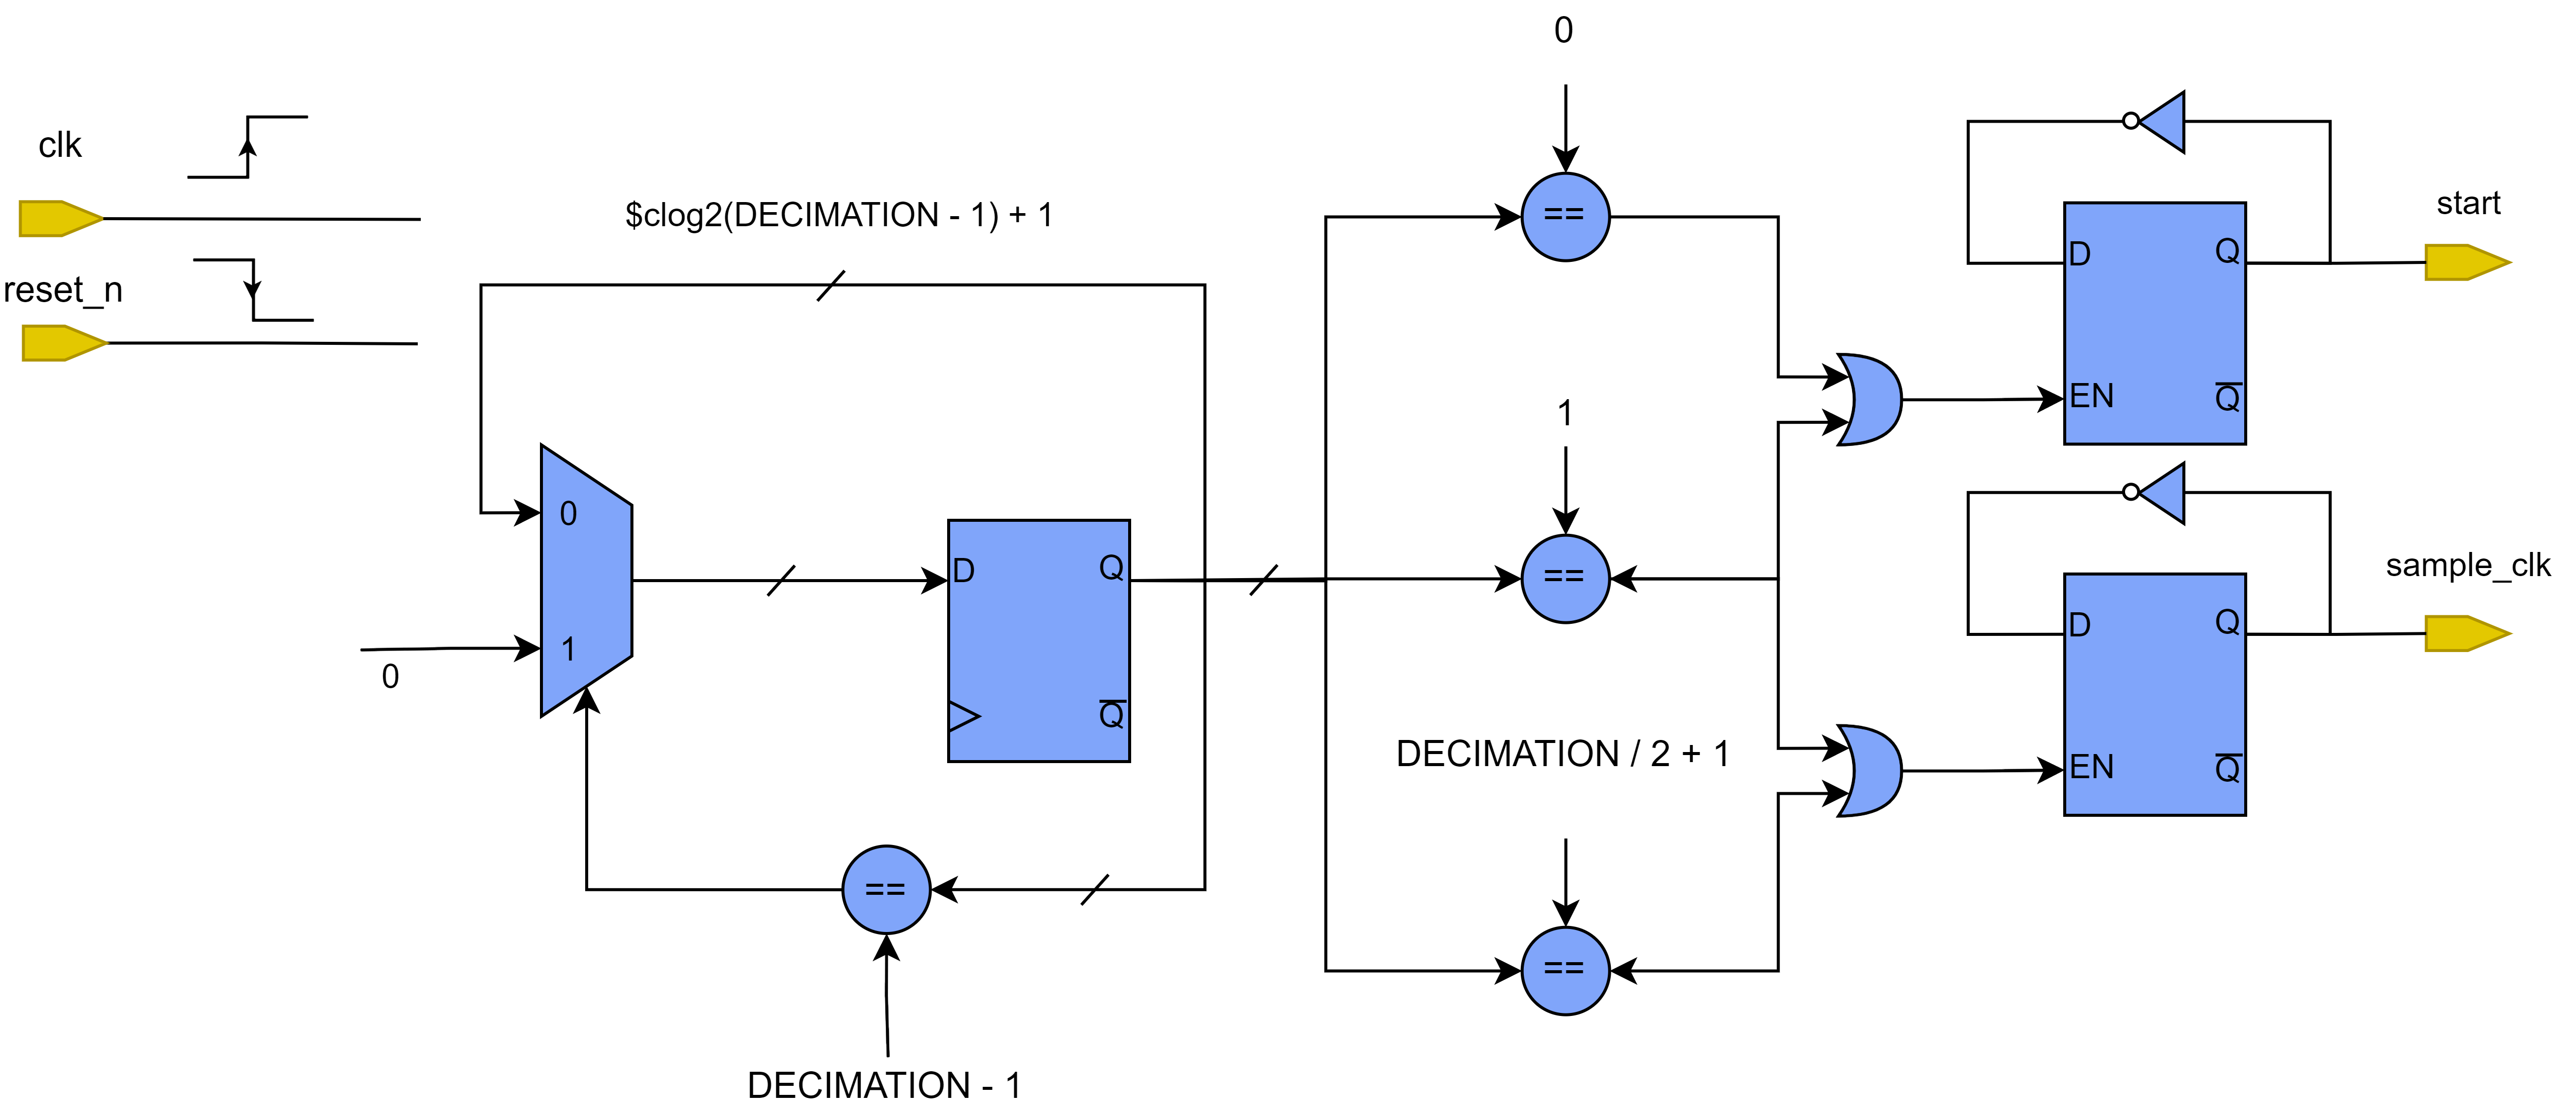
\includegraphics[width=15cm]{Images/Chuong4/frequency/frequency_arc.png}
    \caption[Kiến trúc của dti\_frequency\_divider]{\bfseries \fontsize{12pt}{0pt}\selectfont Kiến trúc của dti\_frequency\_divider}
    \label{frequency_a}
\end{figure}

\paragraph{dti\_top\_frequency\_divider}
\textbf{dti\_top\_frequency\_divider} (hình \ref{top_frequency}) chứa các \textbf{dti\_frequency\_divider} với hệ số DECIMATION 4, 48, 92, 192 để tạo clock và tạo tín hiệu kích hoạt cho bộ lọc.

\begin{figure}[H]
    \centering
    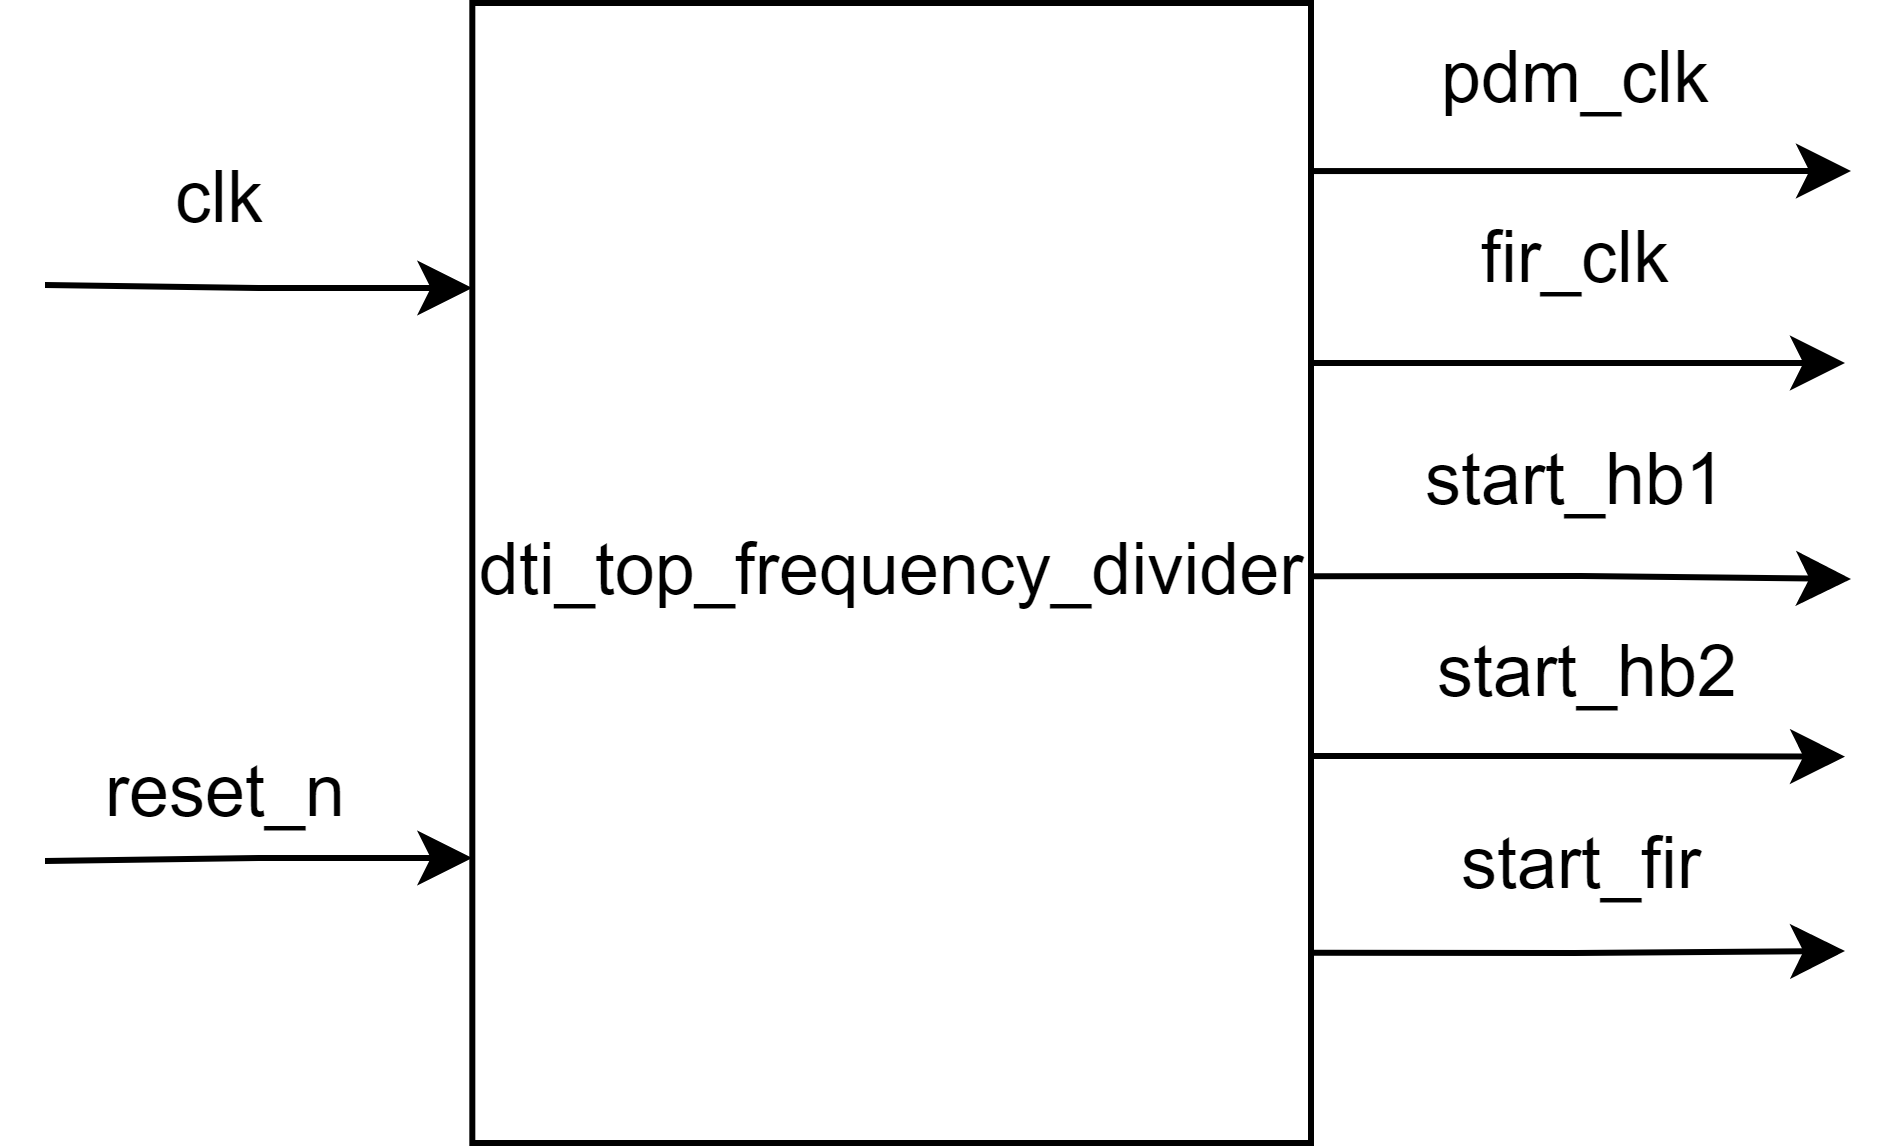
\includegraphics[width=7cm]{Images/Chuong4/frequency/top_frequency.png}
    \caption[Sơ đồ khối của dti\_top\_frequency\_divider]{\bfseries \fontsize{12pt}{0pt}\selectfont Sơ đồ khối của dti\_top\_frequency\_divider}
    \label{top_frequency}
\end{figure}
Kiến trúc của dti\_top\_frequency\_divider gồm 4 bộ dti\_top\_frequency\_divider như hình \ref{top_frequency_arc}.
\begin{figure}[H]
    \centering
    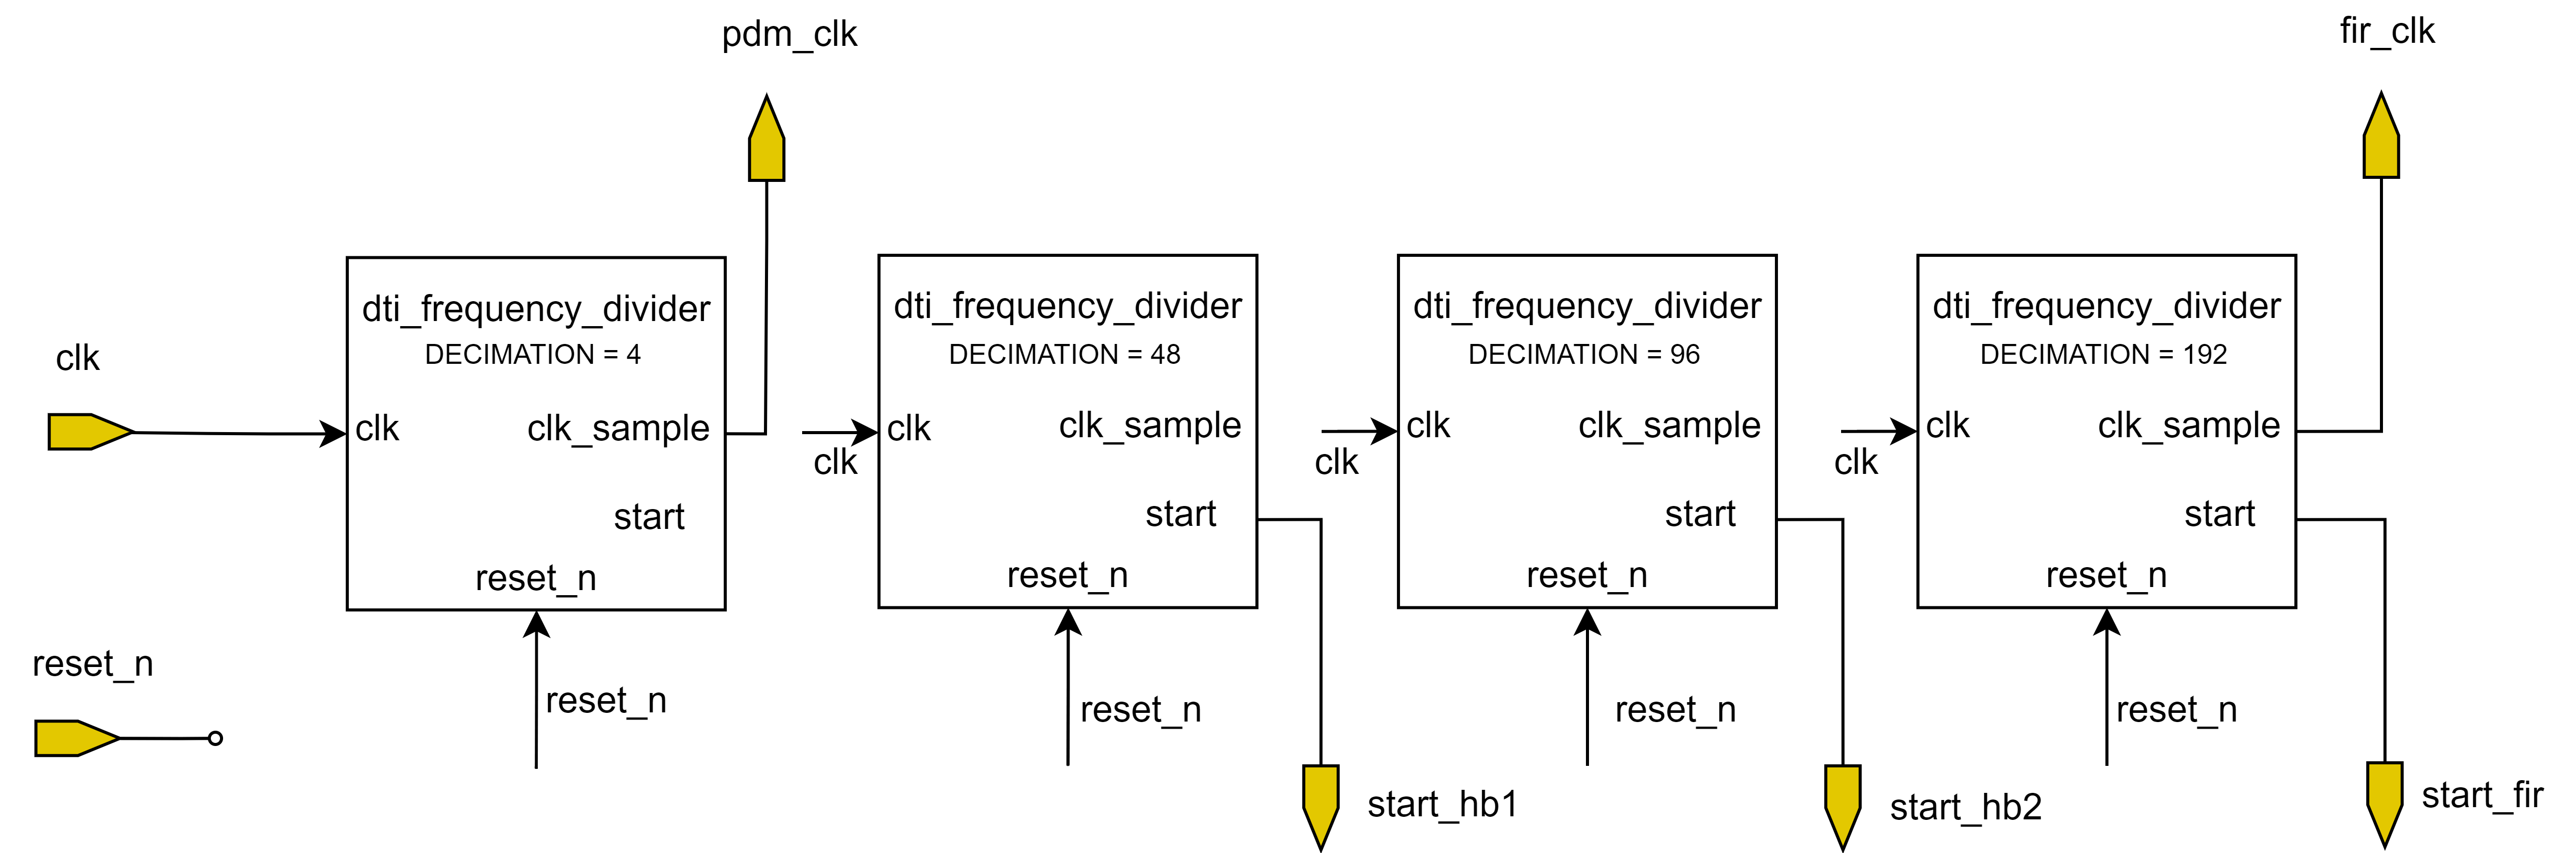
\includegraphics[width=15cm]{Images/Chuong4/frequency/top_frequency_arc.png}
    \caption[Kiến trúc của dti\_top\_frequency\_divider]{\bfseries \fontsize{12pt}{0pt}\selectfont Kiến trúc của dti\_top\_frequency\_divider}
    \label{top_frequency_arc}
\end{figure}


\begin{table}[H]
    \centering
    \caption[Mô tả chân vào ra của dti\_top\_frequency\_divider]{\bfseries\fontsize{12pt}{0pt}\selectfont Mô tả chân vào ra của dti\_top\_frequency\_divider}
    \begin{tabular}{|l|c|c|l|}
\hline
\multicolumn{1}{|c|}{\textbf{Tên chân}} &
  \textbf{Vào/ ra} &
  \textbf{Độ rộng bit} &
  \multicolumn{1}{c|}{\textbf{Mô tả chức năng}} \\ \hline
clk &
  vào &
  1 &
  Clock đồng bộ hoạt động của hệ thống \\ \hline
reset\_n &
  vào &
  1 &
  \begin{tabular}[c]{@{}l@{}}Chân reset không đồng bộ, tích cực mức\\ thấp\end{tabular} \\ \hline
start\_hb1 &
  ra &
  1 &
  \begin{tabular}[c]{@{}l@{}}Tín hiệu điều khiển cho biết liệu dữ liệu \\ có sẵn ở đầu vào của bộ lọc HB1\end{tabular} \\ \hline
start\_hb2 &
  ra &
  1 &
  \begin{tabular}[c]{@{}l@{}}Tín hiệu điều khiển cho biết liệu dữ liệu \\ có sẵn ở đầu vào của bộ lọc HB2\end{tabular} \\ \hline

start\_fir &
  ra &
  1 &
  \begin{tabular}[c]{@{}l@{}}Tín hiệu điều khiển cho biết liệu dữ liệu \\ có sẵn ở đầu vào của bộ lọc FIR\end{tabular} \\ \hline
pdm\_clk &
  ra &
  1 &
  Clock lấy mẫu của PDM \\ \hline
pcm\_clk &
  ra &
  1 &
  Clock lấy mẫu của PCM \\ \hline
  \end{tabular}
    \label{top_frequency_signal}
\end{table}

  Bảng \ref{top_frequency_signal} cho miêu tả chức năng của các chân vào ra của khối. 

\paragraph{dti\_cic\_decimator}
 Như đã trình bày ở mục \ref{cic_filter_ref}, với thiết kế bộ lọc CIC 4 tầng và hệ số Decimation 12x thì chúng ta cần đến 4 bộ cộng và 4 bộ trừ. Chúng ta có thể tăng tần số xử lý lên 4 lần, lúc này chỉ cần sử dụng 1 bộ cộng và 1 bộ trừ, điều này làm giảm tài nguyên phần cứng một cách đáng kể.

Hình \ref{cic_top} mô tả sơ đồ khối của khối dti\_cic\_decimator.
\begin{figure}[H]
    \centering
    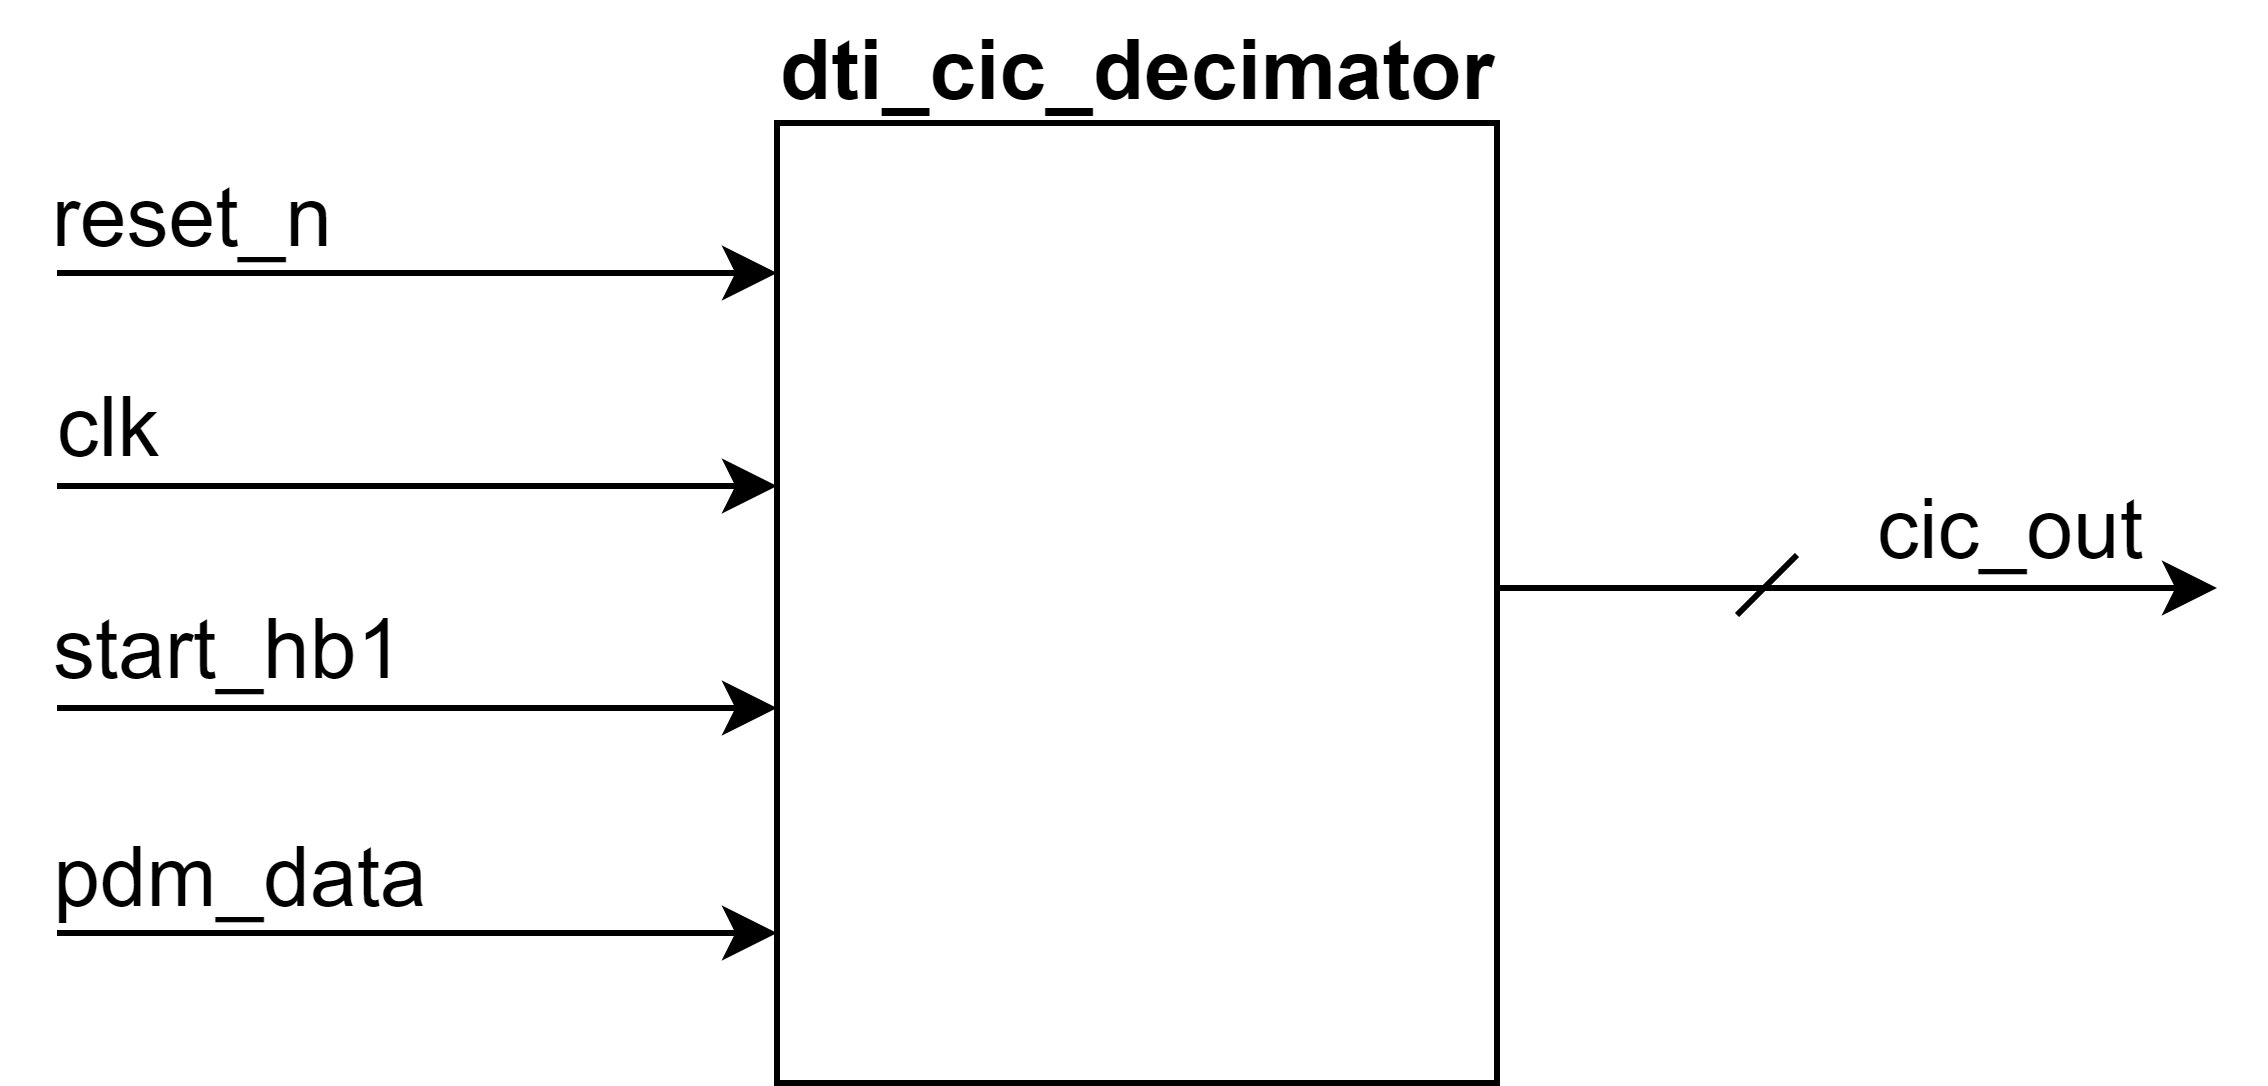
\includegraphics[width=10cm]{Images/Chuong4/cic/cic_top.png}
    \caption[Sơ đồ khối của dti\_cic\_decimator]{\bfseries \fontsize{12pt}{0pt}\selectfont Sơ đồ khối của dti\_cic\_decimator}
    \label{cic_top}
\end{figure}

Việc tính toán độ rông bit cho các thanh ghi trễ được tính toán theo công thức \ref{bitcic}. Với số tầng là 4 và hệ số Decimation 12x ta có độ rộng bit như sau:
\begin{equation}
    n_r = 1 + [4 \times log_2(2 \times 12)] = 16 (bits)
\end{equation}
\begin{table}[H]
    \centering
    \caption[Mô tả chân vào ra của dti\_cic\_decimator]{\bfseries\fontsize{12pt}{0pt}\selectfont Mô tả chân vào ra của dti\_cic\_decimator}
    \begin{tabular}{|l|c|c|l|}
\hline
\multicolumn{1}{|c|}{\textbf{Tên chân}} &
  \textbf{Vào/ ra} &
  \textbf{Độ rộng bit} &
  \multicolumn{1}{c|}{\textbf{Mô tả chức năng}} \\ \hline
clk       & vào & 1 & Clock đồng bộ hoạt động của hệ thống \\ \hline
reset\_n &
  vào &
  1 &
  \begin{tabular}[c]{@{}l@{}}Chân reset không đồng bộ, tích cực mức\\ thấp\end{tabular} \\ \hline
start\_hb1 &
  vào &
  1 &
  \begin{tabular}[c]{@{}l@{}}Báo hiệu rằng dữ liệu đầu ra CIC thay đổi\\ (bộ lọc HB1 nhận dữ liệu)\end{tabular} \\ \hline
pdm\_data & vào & 1 & Dữ liệu PDM đầu vào                  \\ \hline
pcm\_data &
  ra &
  16 &
  \begin{tabular}[c]{@{}l@{}}Đầu ra của bộ lọc CIC, tiếp tục đưa vào \\ bộ lọc HB1\end{tabular} \\ \hline
\end{tabular}
    \label{cic_top_t}
\end{table}

Bảng \ref{cic_top_t} liệt kê các cổng vào ra của khối dti\_cic\_decimator. Khi chỉ sử dụng 1 bộ cộng và 1 bộ trừ, chúng ta phải phân công theo từng thời gian tính toán các phép tính 1 cách hợp lý, hình \ref{cic_top_arc} mô tả kiến trúc đáp ứng được điều kiện trên.

\begin{figure}[H]
    \centering
    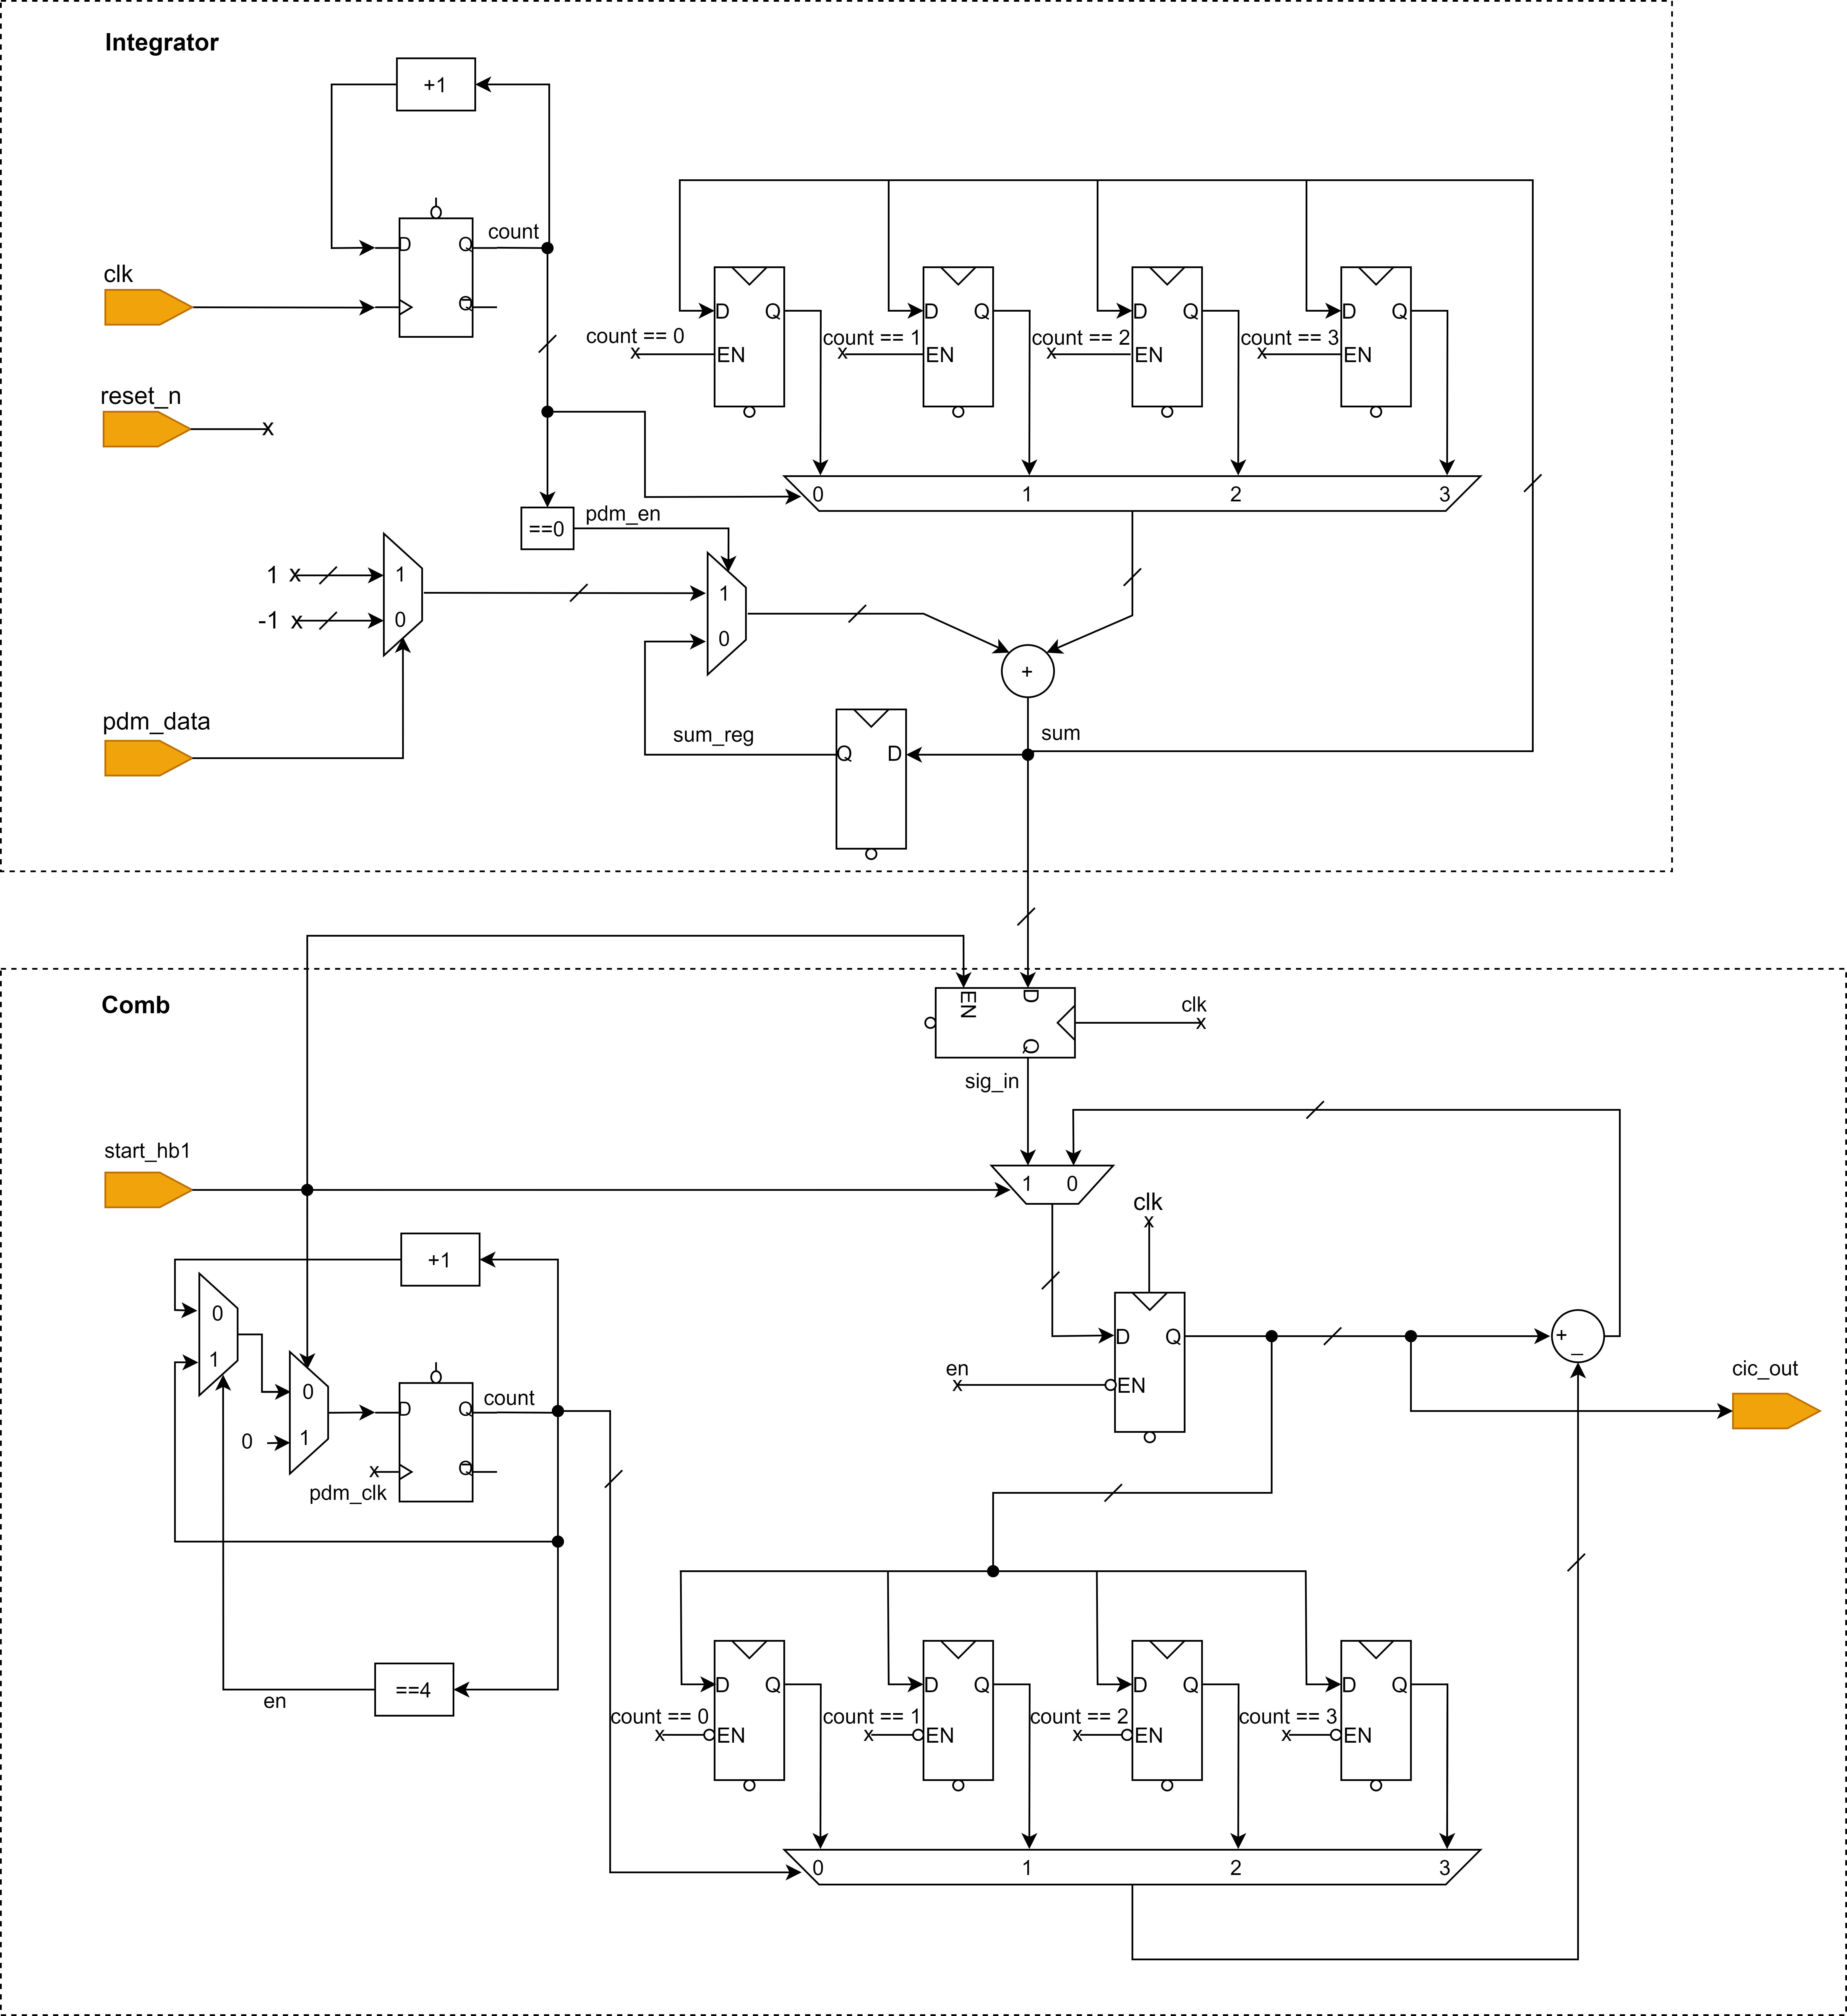
\includegraphics[width=16cm]{Images/Chuong4/cic/cic_top_arc.png}
    \caption[Kiến trúc của dti\_cic\_decimator]{\bfseries \fontsize{12pt}{0pt}\selectfont Kiến trúc của dti\_cic\_decimator}
    \label{cic_top_arc}
\end{figure}
 \paragraph{dti\_hb\_fir\_filter}
Tương tự bộ lọc CIC, 3 bộ lọc tiếp theo cũng phải sử dụng số bộ nhân và bộ cộng nhất định:
\begin{itemize}
    \item Half Band (1): có 11 taps, trong đó 4 taps có hệ số bằng 0 coi như không sử dụng bộ nhân ở đây. Đồng nghĩa với việc chúng ta cần phải có 7 bộ nhân và 10 bộ cộng cho bộ HB1.
     \item Half Band (2): có 19 taps. Tương tự cách tính của HB1, HB2 cần 11 bộ nhân và 18 bộ cộng.
     \item FIR: có 51 taps nên sẽ sửa dụng 51 bộ nhân và 50 bộ cộng.
\end{itemize} 

Không những thế bộ nhân là bộ có kích thước khá lớn, việc sử dụng số lượng nhiều sẽ gây tiêu tốn tài nguyên. Ý tưởng của kiến trúc này là chỉ sử dụng 1 bộ nhân duy nhất cho 3 bộ lọc và mỗi bộ lọc sử dụng 2 bộ cộng.

\begin{figure}[H]
    \centering
    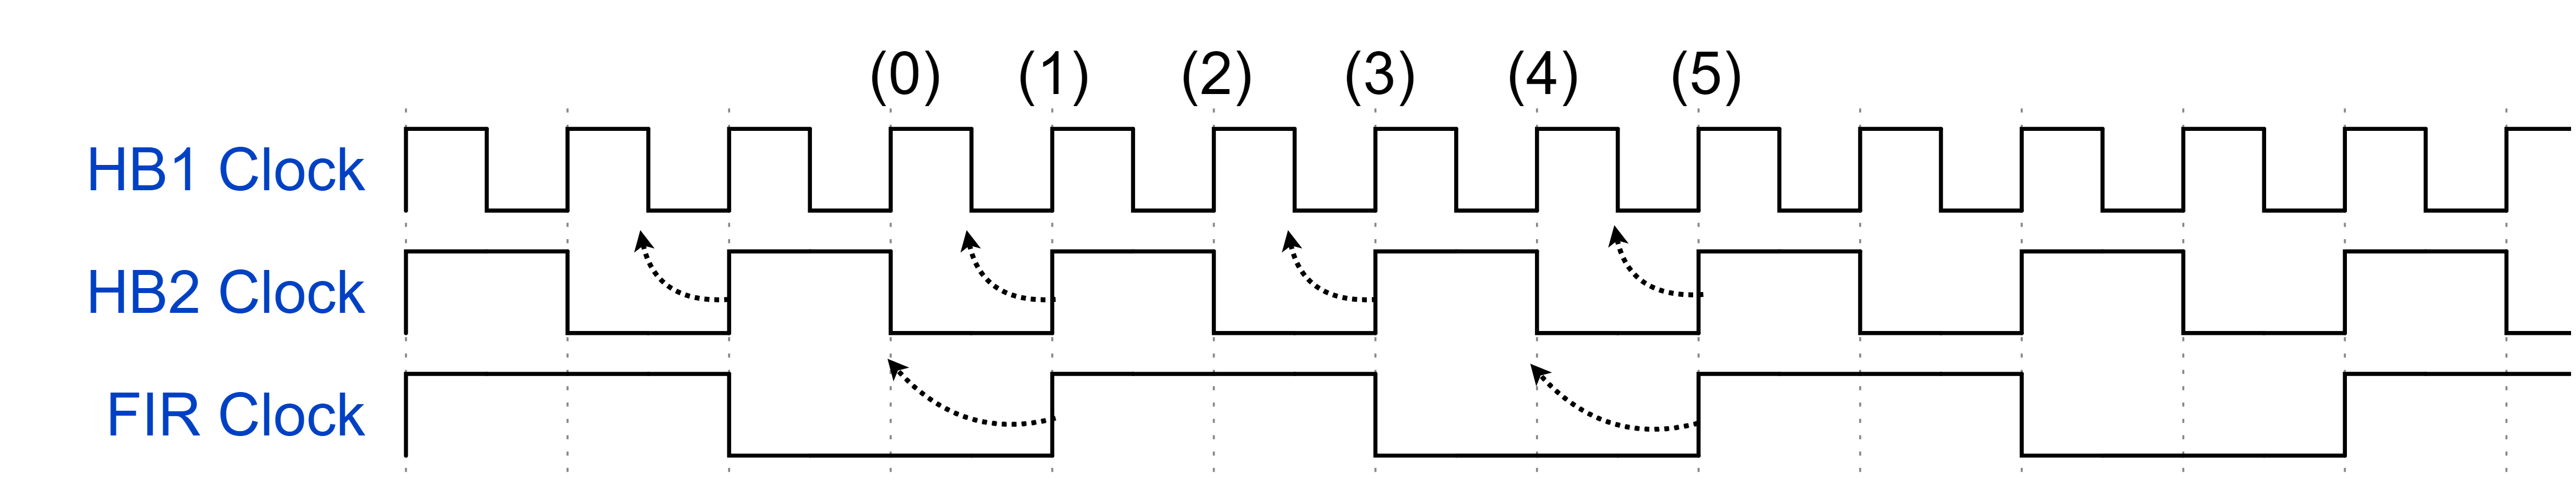
\includegraphics[width=16cm]{Images/Chuong4/hb_fir/timing.png}
    \caption[Biểu đồ thời gian của 3 clock của 3 bộ lọc]{\bfseries \fontsize{12pt}{0pt}\selectfont Biểu đồ thời gian của 3 clock của 3 bộ lọc}
    \label{3clock}
\end{figure}

Quan sát biểu đồ thời gian của 3 clock (hình \ref{3clock}), ta có nhận xét sau: không phải tất cả ở sườn dương nào thì các bộ lọc đều phải tính toán. Việc tính toán hay không là do bộ lọc sau lấy giá trị ở thời điểm nào để tính toán. Ví dụ với bộ lọc HB2, nó chỉ lấy giá trị đầu ra của HB1 sau thời điểm (0), (2), (4) điều này đồng nghĩa với việc ở đây HB1 phải thực hiện các phép toán ở (0), (2), (4) để xuất tín hiệu cho đầu vào HB2, ở các điểm còn lại HB1 chỉ cần dịch giá trị đầu vào vào và không làm thêm gì. Điều đó tương tự với bộ lọc FIR, nó chỉ lấy đầu vào của HB2  sau thời điểm (3) để tính toán.

Dựa vào cách hoạt động trên, ta có thể tiến hành để mỗi bộ lọc sử dụng bộ nhân ở 1 thời điểm nhất định. Với ví dụ trên thứ tự sử dụng bộ nhân sẽ như sau: (0) - HB1, (1) - FIR, (2) - HB1, (3) - HB2 và lặp lại. Việc phân luồng sẽ có do bộ \textbf{dti\_filter\_controller} điều khiển.

Do bộ FIR sẽ có 52 taps, đồng nghĩa với việc trong 1 chu kỳ của HB1 phải thực hiện xong 26 lần nhân (vì hệ số đối xứng). Ta xét tần số hoạt động của HB1 là 192 kHz thì tần hoạt động của bộ nhân phải là $192 \times 26 = 4492 kHz$. Với tần số của hệ thống sử dụng (dti\_cic\_decimatior clock) là 9216 khz đã hoàn toàn đáp ứng được.

\begin{figure}[H]
    \centering
    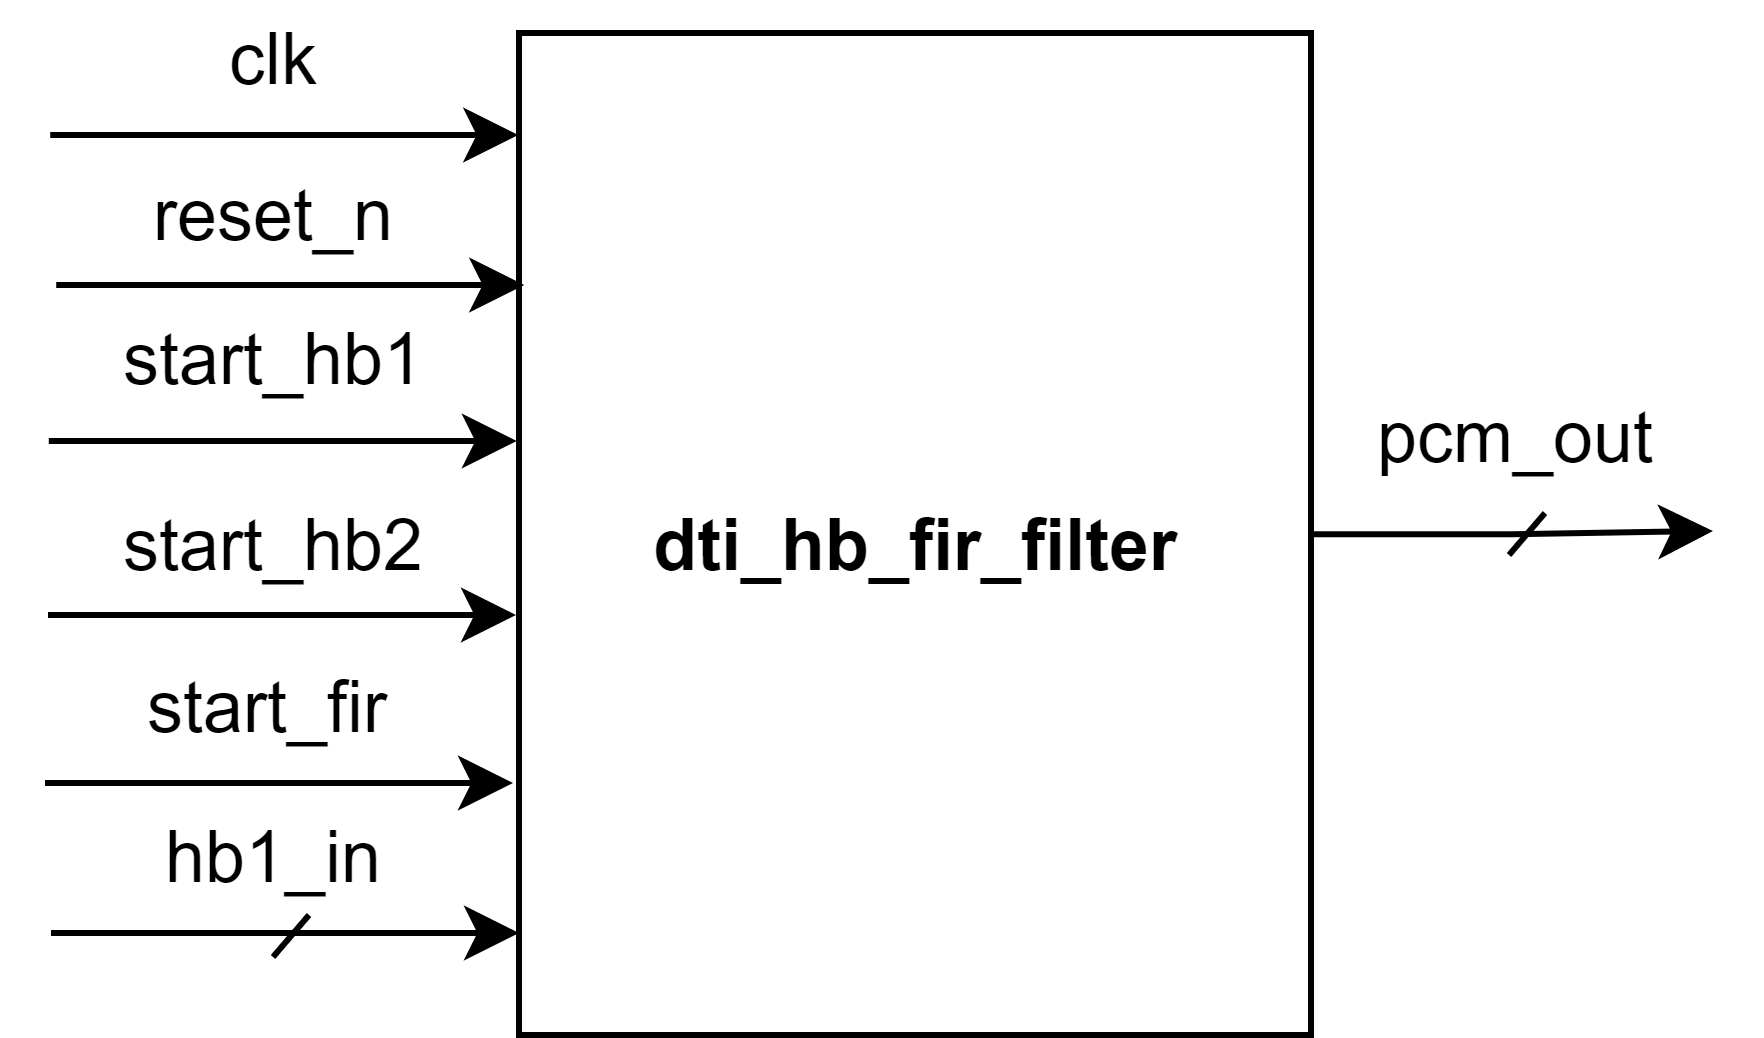
\includegraphics[width=8cm]{Images/Chuong4/hb_fir/hb_fir_top.png}
    \caption[Sơ đồ khối của dti\_cic\_decimator]{\bfseries \fontsize{12pt}{0pt}\selectfont Sơ đồ khối của dti\_hb\_fir\_filter}
    \label{hb_fir_top}
\end{figure}
Hình \ref{hb_fir_top} mô tả sơ đồ khối của khối dti\_hb\_fir\_filter.

\begin{table}[H]
    \centering
    \caption[Mô tả chân vào ra của dti\_hb\_fir\_filter]{\bfseries\fontsize{12pt}{0pt}\selectfont Mô tả chân vào ra của dti\_hb\_fir\_filter}
    \begin{tabular}{|l|c|c|l|}
\hline
\multicolumn{1}{|c|}{\textbf{Tên chân}} & \textbf{Vào/ ra} & \textbf{Độ rộng bit} & \multicolumn{1}{c|}{\textbf{Mô tả chức năng}} \\ \hline
clk        & vào & 1          & Clock đồng bộ hoạt động của hệ thống                                                        \\ \hline
reset\_n   & vào & 1          & \begin{tabular}[c]{@{}l@{}}Chân reset không đồng bộ, tích cực mức\\ thấp\end{tabular}       \\ \hline
start\_hb1 & vào & 1          & \begin{tabular}[c]{@{}l@{}}Báo hiệu rằng dữ liệu đầu vào HB1 là\\ giá trị mới\end{tabular}  \\ \hline
start\_hb1 & vào & 1          & \begin{tabular}[c]{@{}l@{}}Báo hiệu rằng dữ liệu đầu vào HB2 là \\ giá trị mới\end{tabular} \\ \hline
start\_fir & vào & 1          & \begin{tabular}[c]{@{}l@{}}Báo hiệu rằng dữ liệu đầu vào FIR là\\ giá trị mới\end{tabular}  \\ \hline
hb1\_in    & vào & CIC\_WIDTH & Dữ liệu đầu vào của bộ lọc HB1                                                              \\ \hline
pcm\_data  & ra  & PCM\_WIDTH & Tín hiệu PCM đầu ra                                                                         \\ \hline
\end{tabular}
    \label{hb_fir_t}
\end{table}

\begin{table}[H]
    \centering
    \caption[Hằng số thiết kế của dti\_hb\_fir\_filter]{\bfseries\fontsize{12pt}{0pt}\selectfont Hằng số thiết kế của dti\_hb\_fir\_filter}
\begin{tabular}{|l|c|l|}
\hline
\multicolumn{1}{|c|}{\textbf{Hằng số}} & \textbf{Giá trị} & \multicolumn{1}{c|}{\textbf{Mô tả}} \\ \hline
PCM\_WIDTH  & 24 & Độ rộng của tín hiệu PCM đầu ra \\ \hline
CIC\_WIDTH  & 16 & Độ rộng của đầu ra của bộ lọc CIC \\ \hline
MULP\_WIDTH & 21 & Kích thước đầu vào của bộ nhân \\ \hline
FIR\_SIZE   & 51 & Số lượng taps của bộ lọc FIR    \\ \hline
HB1\_SIZE   & 11 & Số lượng taps của bộ lọc HB1    \\ \hline
HB2\_SIZE   & 19 & Số lượng taps của bộ lọc HB2    \\ \hline
SHIFT\_NUMBER   & 20 & Số lần dịch phải sau mỗi tầng lọc    \\ \hline
HB1\_SUM\_OUT\_WIDTH   & 36 & Độ rộng dữ liệu đầu ra của bộ lọc HB1    \\ \hline
HB2\_SUM\_OUT\_WIDTH   & 37 & Độ rộng dữ liệu đầu ra của bộ lọc HB2    \\ \hline
FIR\_SUM\_OUT\_WIDTH   & 37 & Độ rộng dữ liệu đầu ra của bộ lọc FIR    \\ \hline
\end{tabular}
    \label{hangso_hb_fir}
\end{table}

Trong đó việc tối ưu độ rộng của đầu ra của các bộ lọc (độ rộng của bộ cộng cuối cùng của dãy). Để tìm được giá trị tối ưu nhất, chúng ta đưa đầu vào lớn nhất và nhỏ nhất của đầu vào (đầu vào CIC 16 bit có dải giá trị [20736, -20736]), tiến hành nhân số bé nhất cho đáp ứng xung có giá trị âm và ngược lại. Lúc này đầu ra của từng tầng lọc sẽ có dải giá trị tương ứng với số bit biểu diễn nó như bảng \ref{hangso_hb_fir}. Độ rộng của bộ nhân được là giá trị biểu diễn từ hệ số của taps đã nêu ở mục \ref{fix-fil}.

\begin{figure}[H]
    \centering
    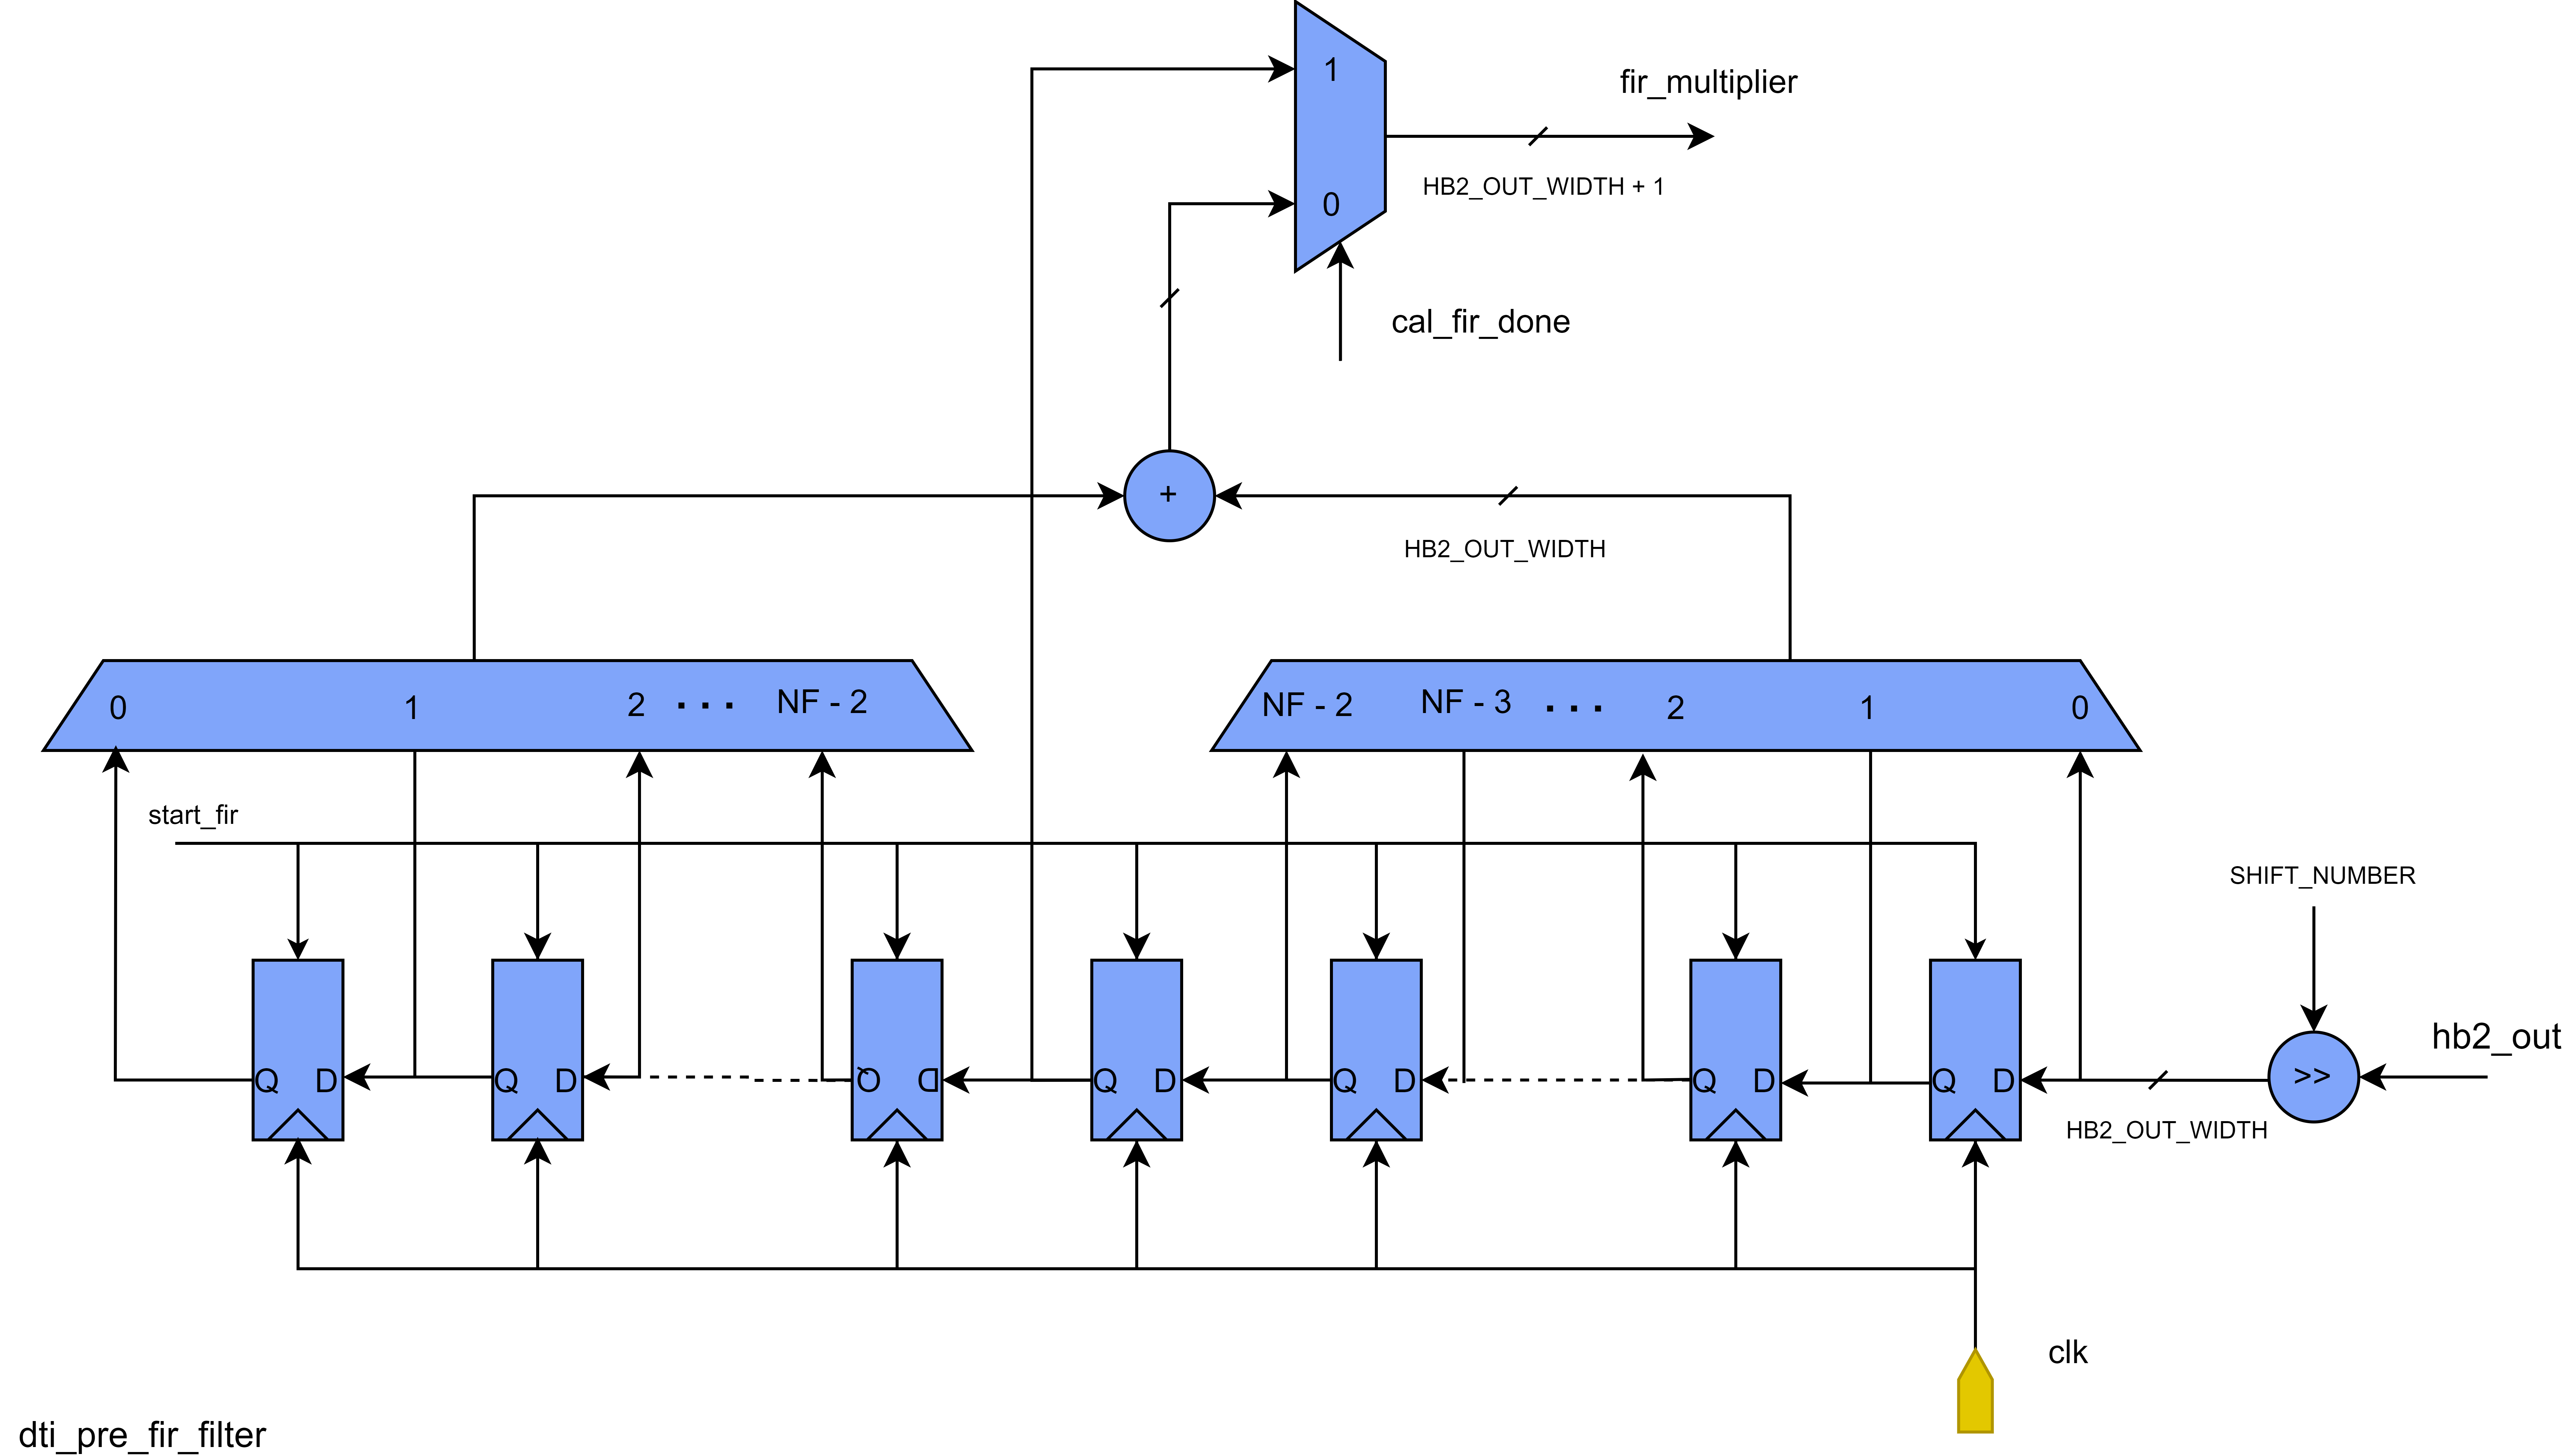
\includegraphics[width=15cm]{Images/Chuong4/hb_fir/pre_fir.png}
    \caption[Kiến trúc của khối liên quan đến bộ lọc FIR trong dti\_hb\_fir\_filter (1)]{\bfseries \fontsize{12pt}{0pt}\selectfont Kiến trúc của khối liên quan đến bộ lọc FIR trong dti\_hb\_fir\_filter (1)}
    \label{pre}
\end{figure}
\begin{figure}[H]
    \centering
    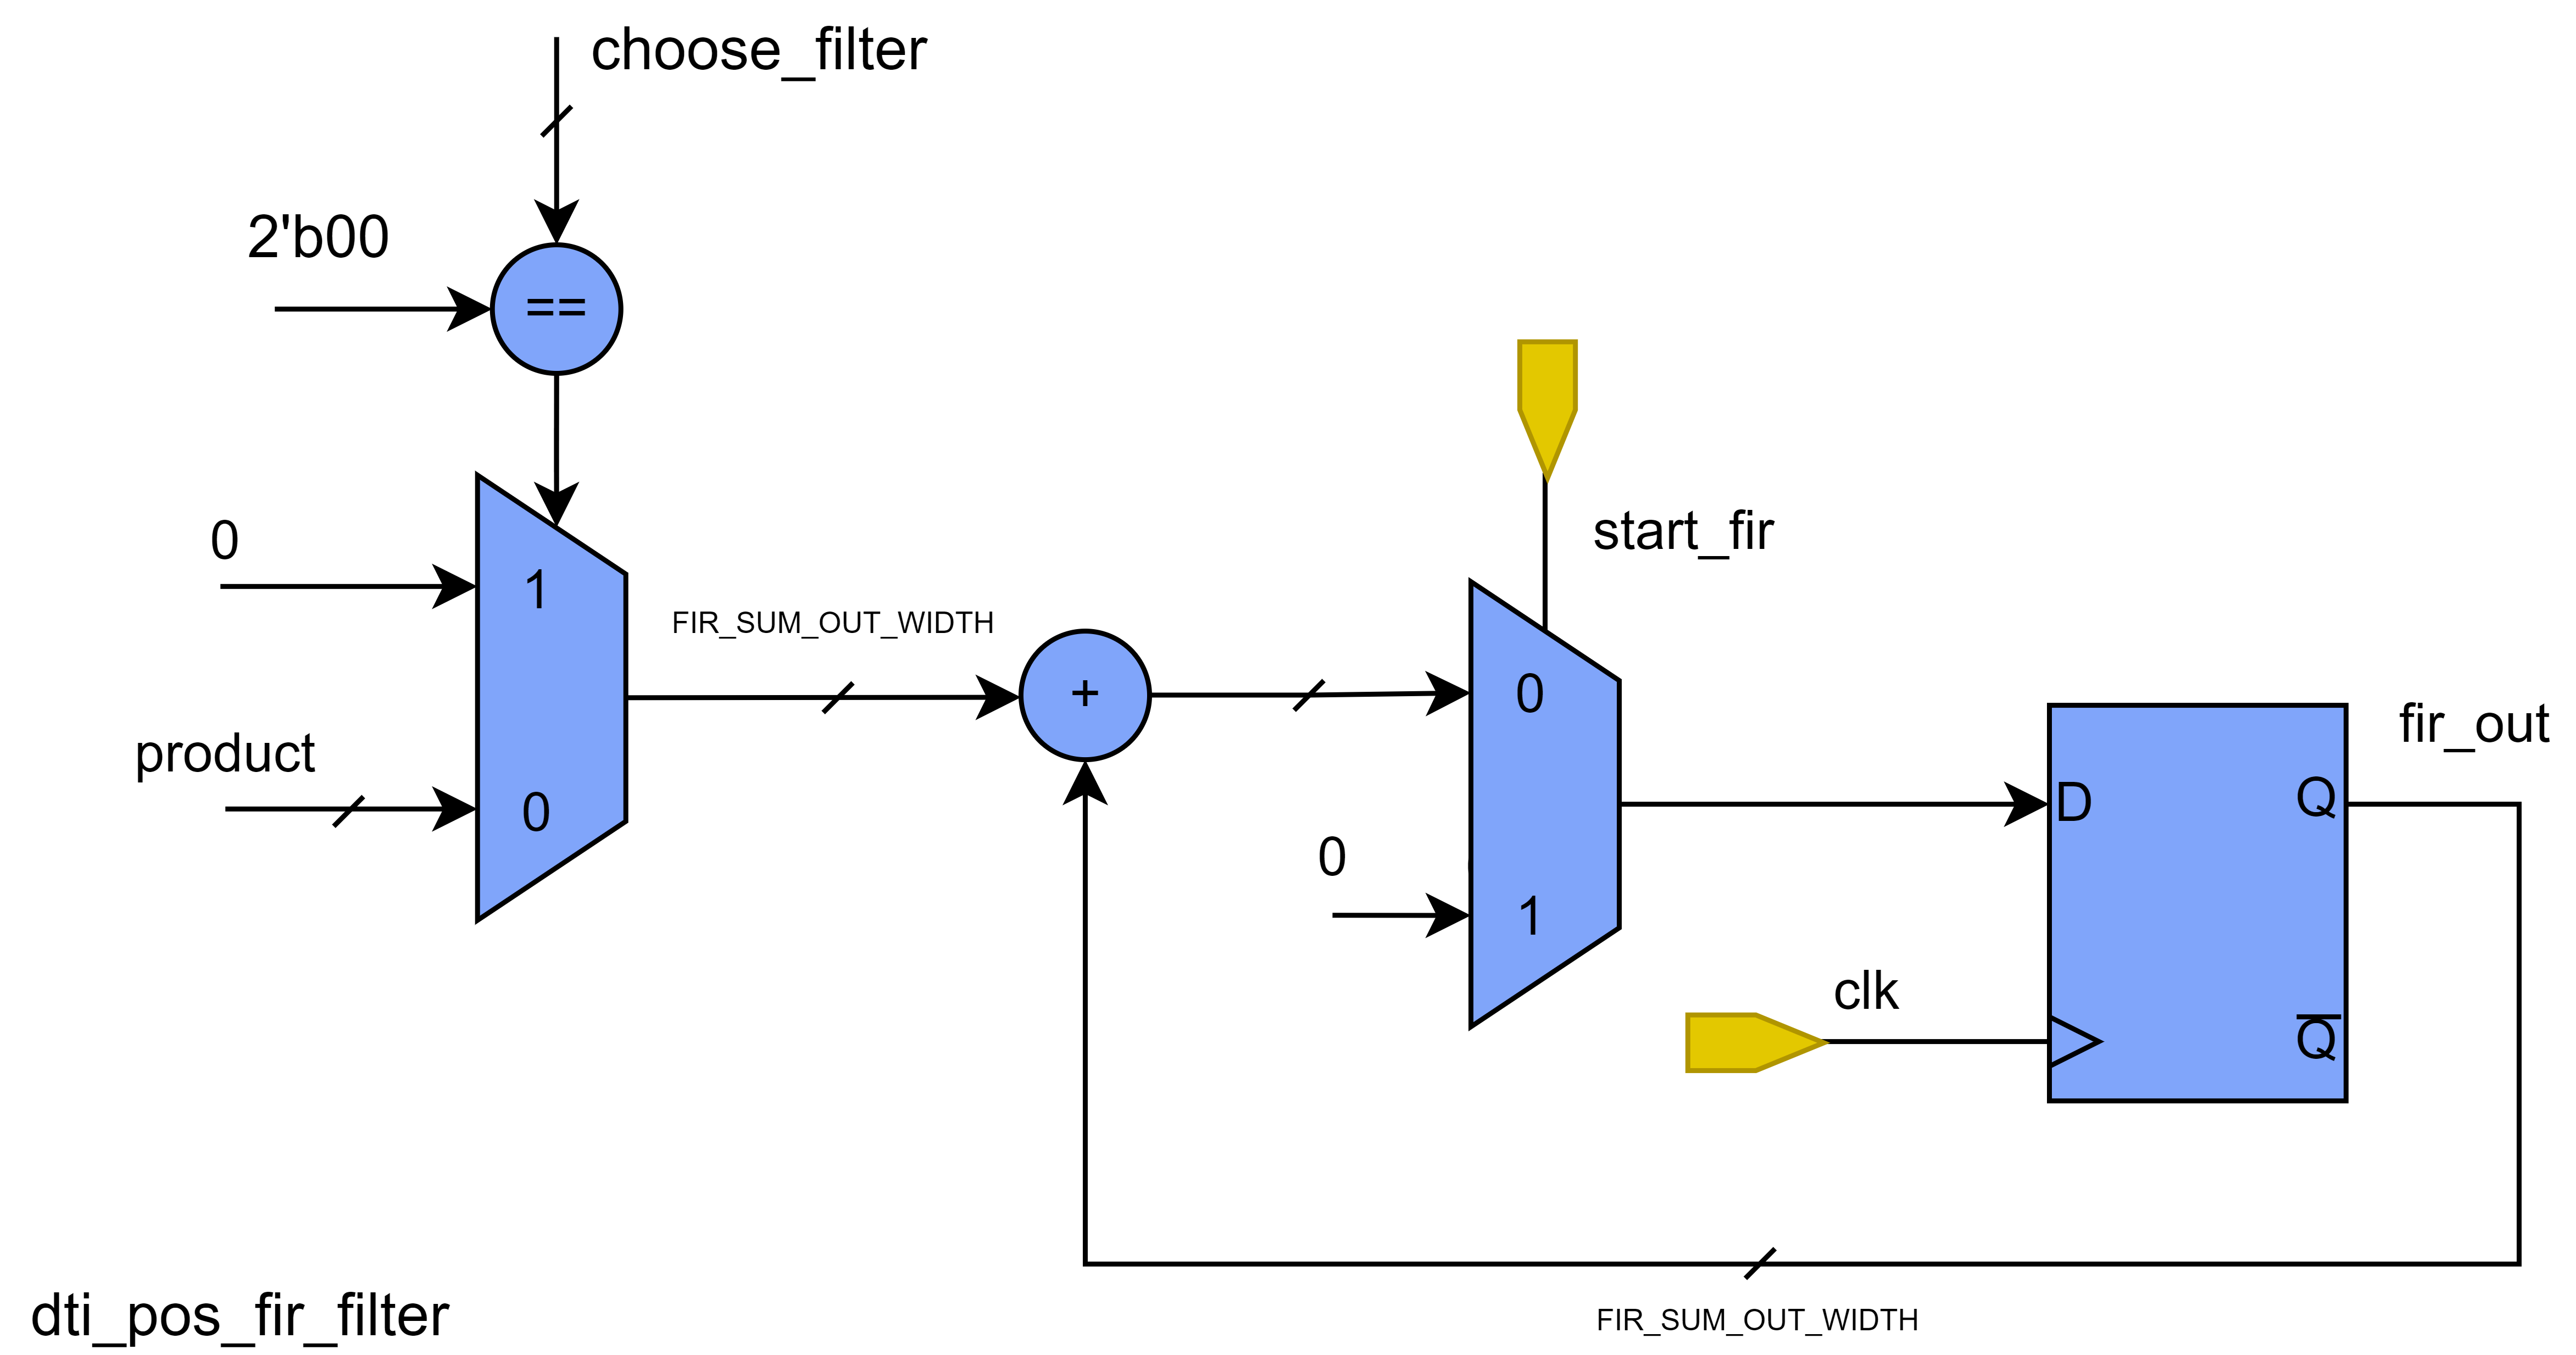
\includegraphics[width=11cm]{Images/Chuong4/hb_fir/pos_fir.png}
    \caption[Kiến trúc của khối liên quan đến bộ lọc FIR trong dti\_hb\_fir\_filter (2)]{\bfseries \fontsize{12pt}{0pt}\selectfont Kiến trúc của khối liên quan đến bộ lọc FIR trong dti\_hb\_fir\_filter (2)}
    \label{pos}
\end{figure}

\begin{figure}[H]
    \centering
    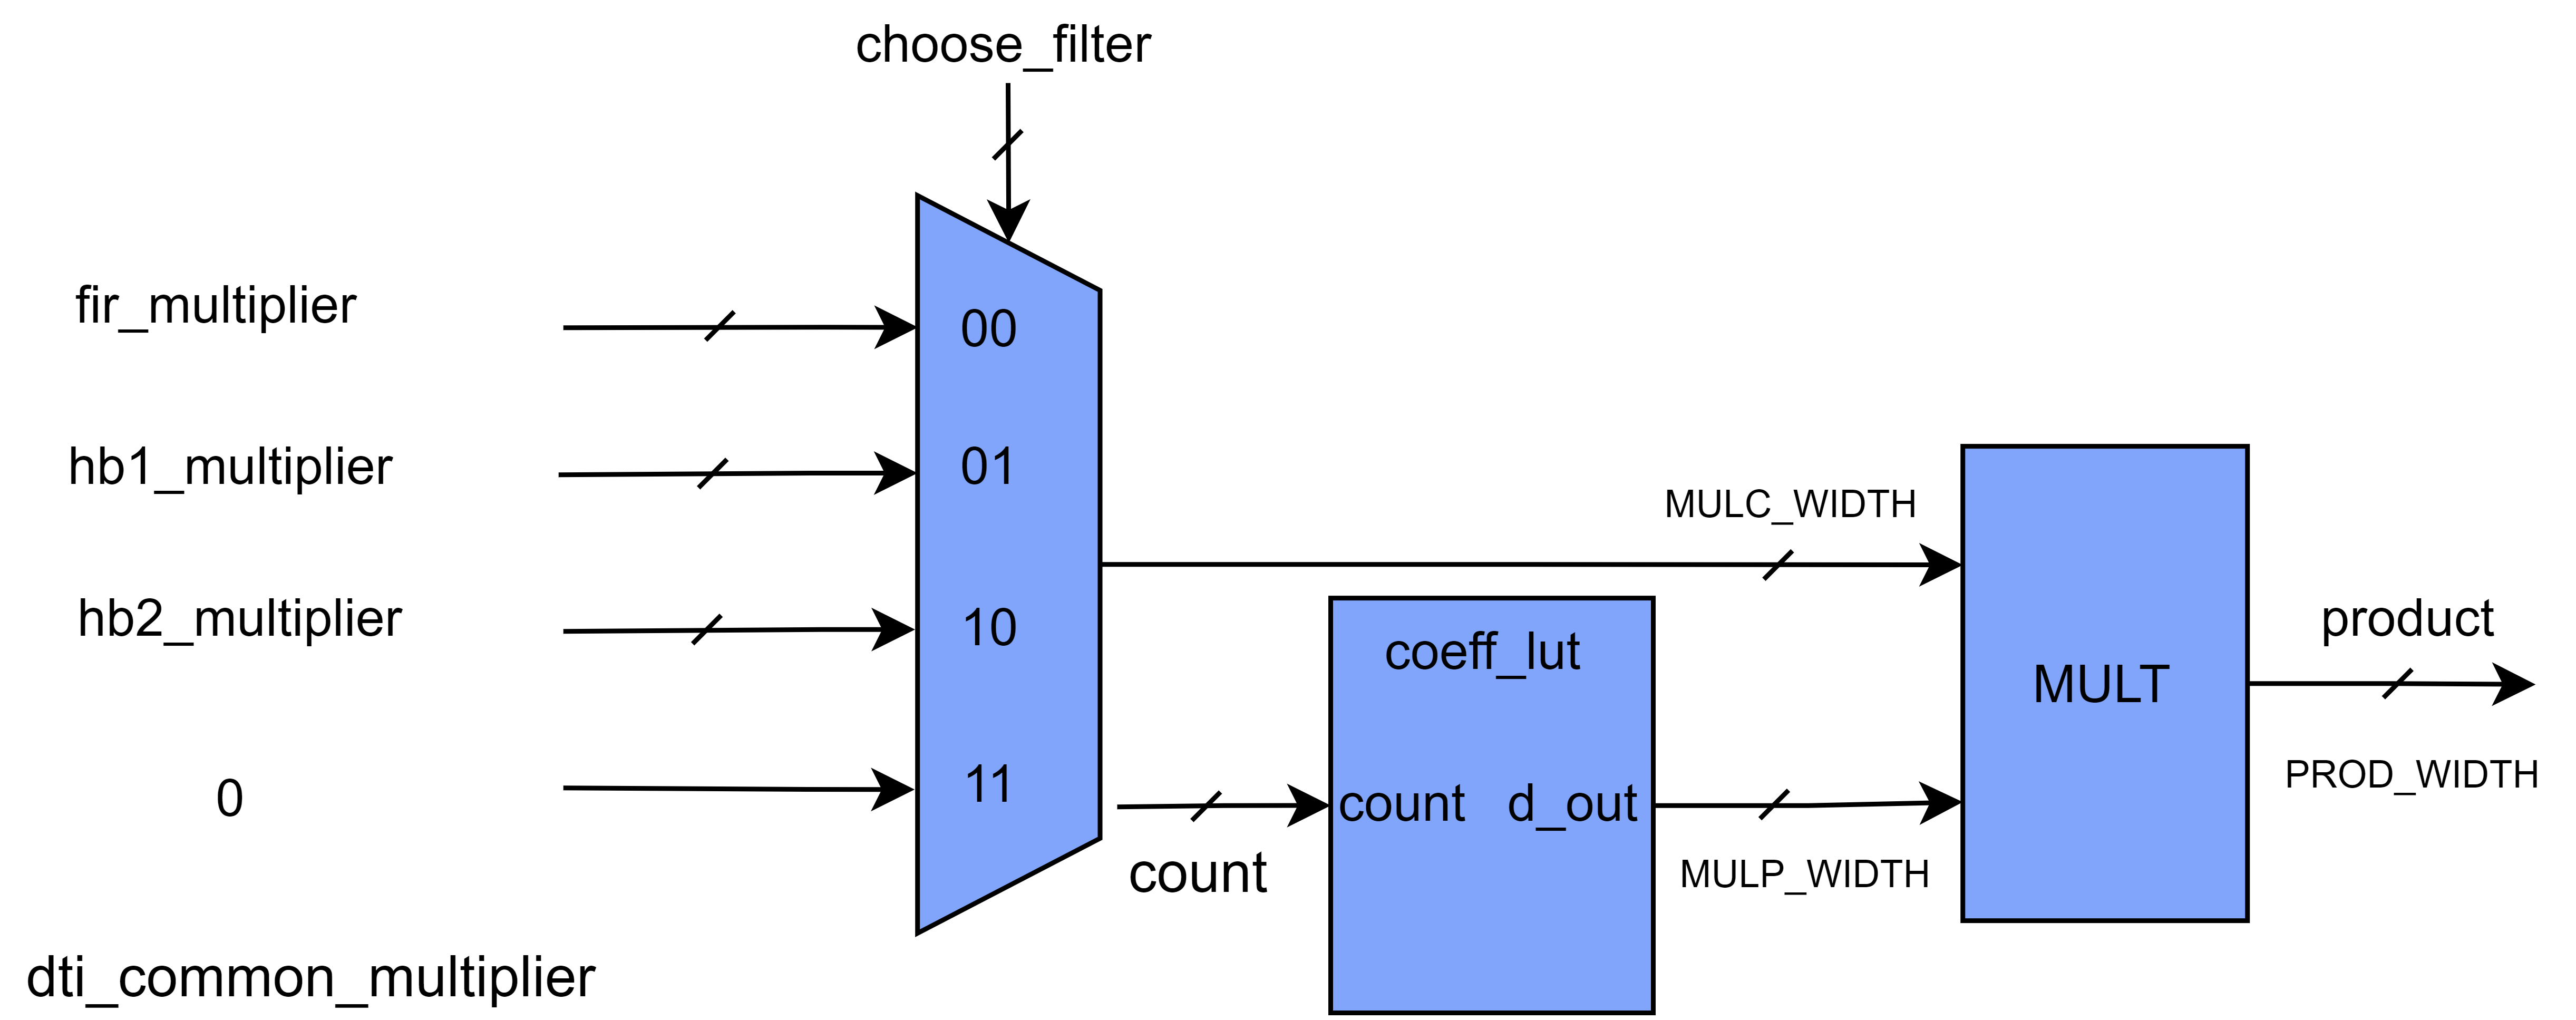
\includegraphics[width=11cm]{Images/Chuong4/hb_fir/mul.png}
    \caption[Kiến trúc khối bộ nhân chung trong dti\_hb\_fir\_filter]{\bfseries \fontsize{12pt}{0pt}\selectfont Kiến trúc khối bộ nhân chung trong dti\_hb\_fir\_filter}
    \label{c_mul}
\end{figure}

\begin{figure}[H]
    \centering
    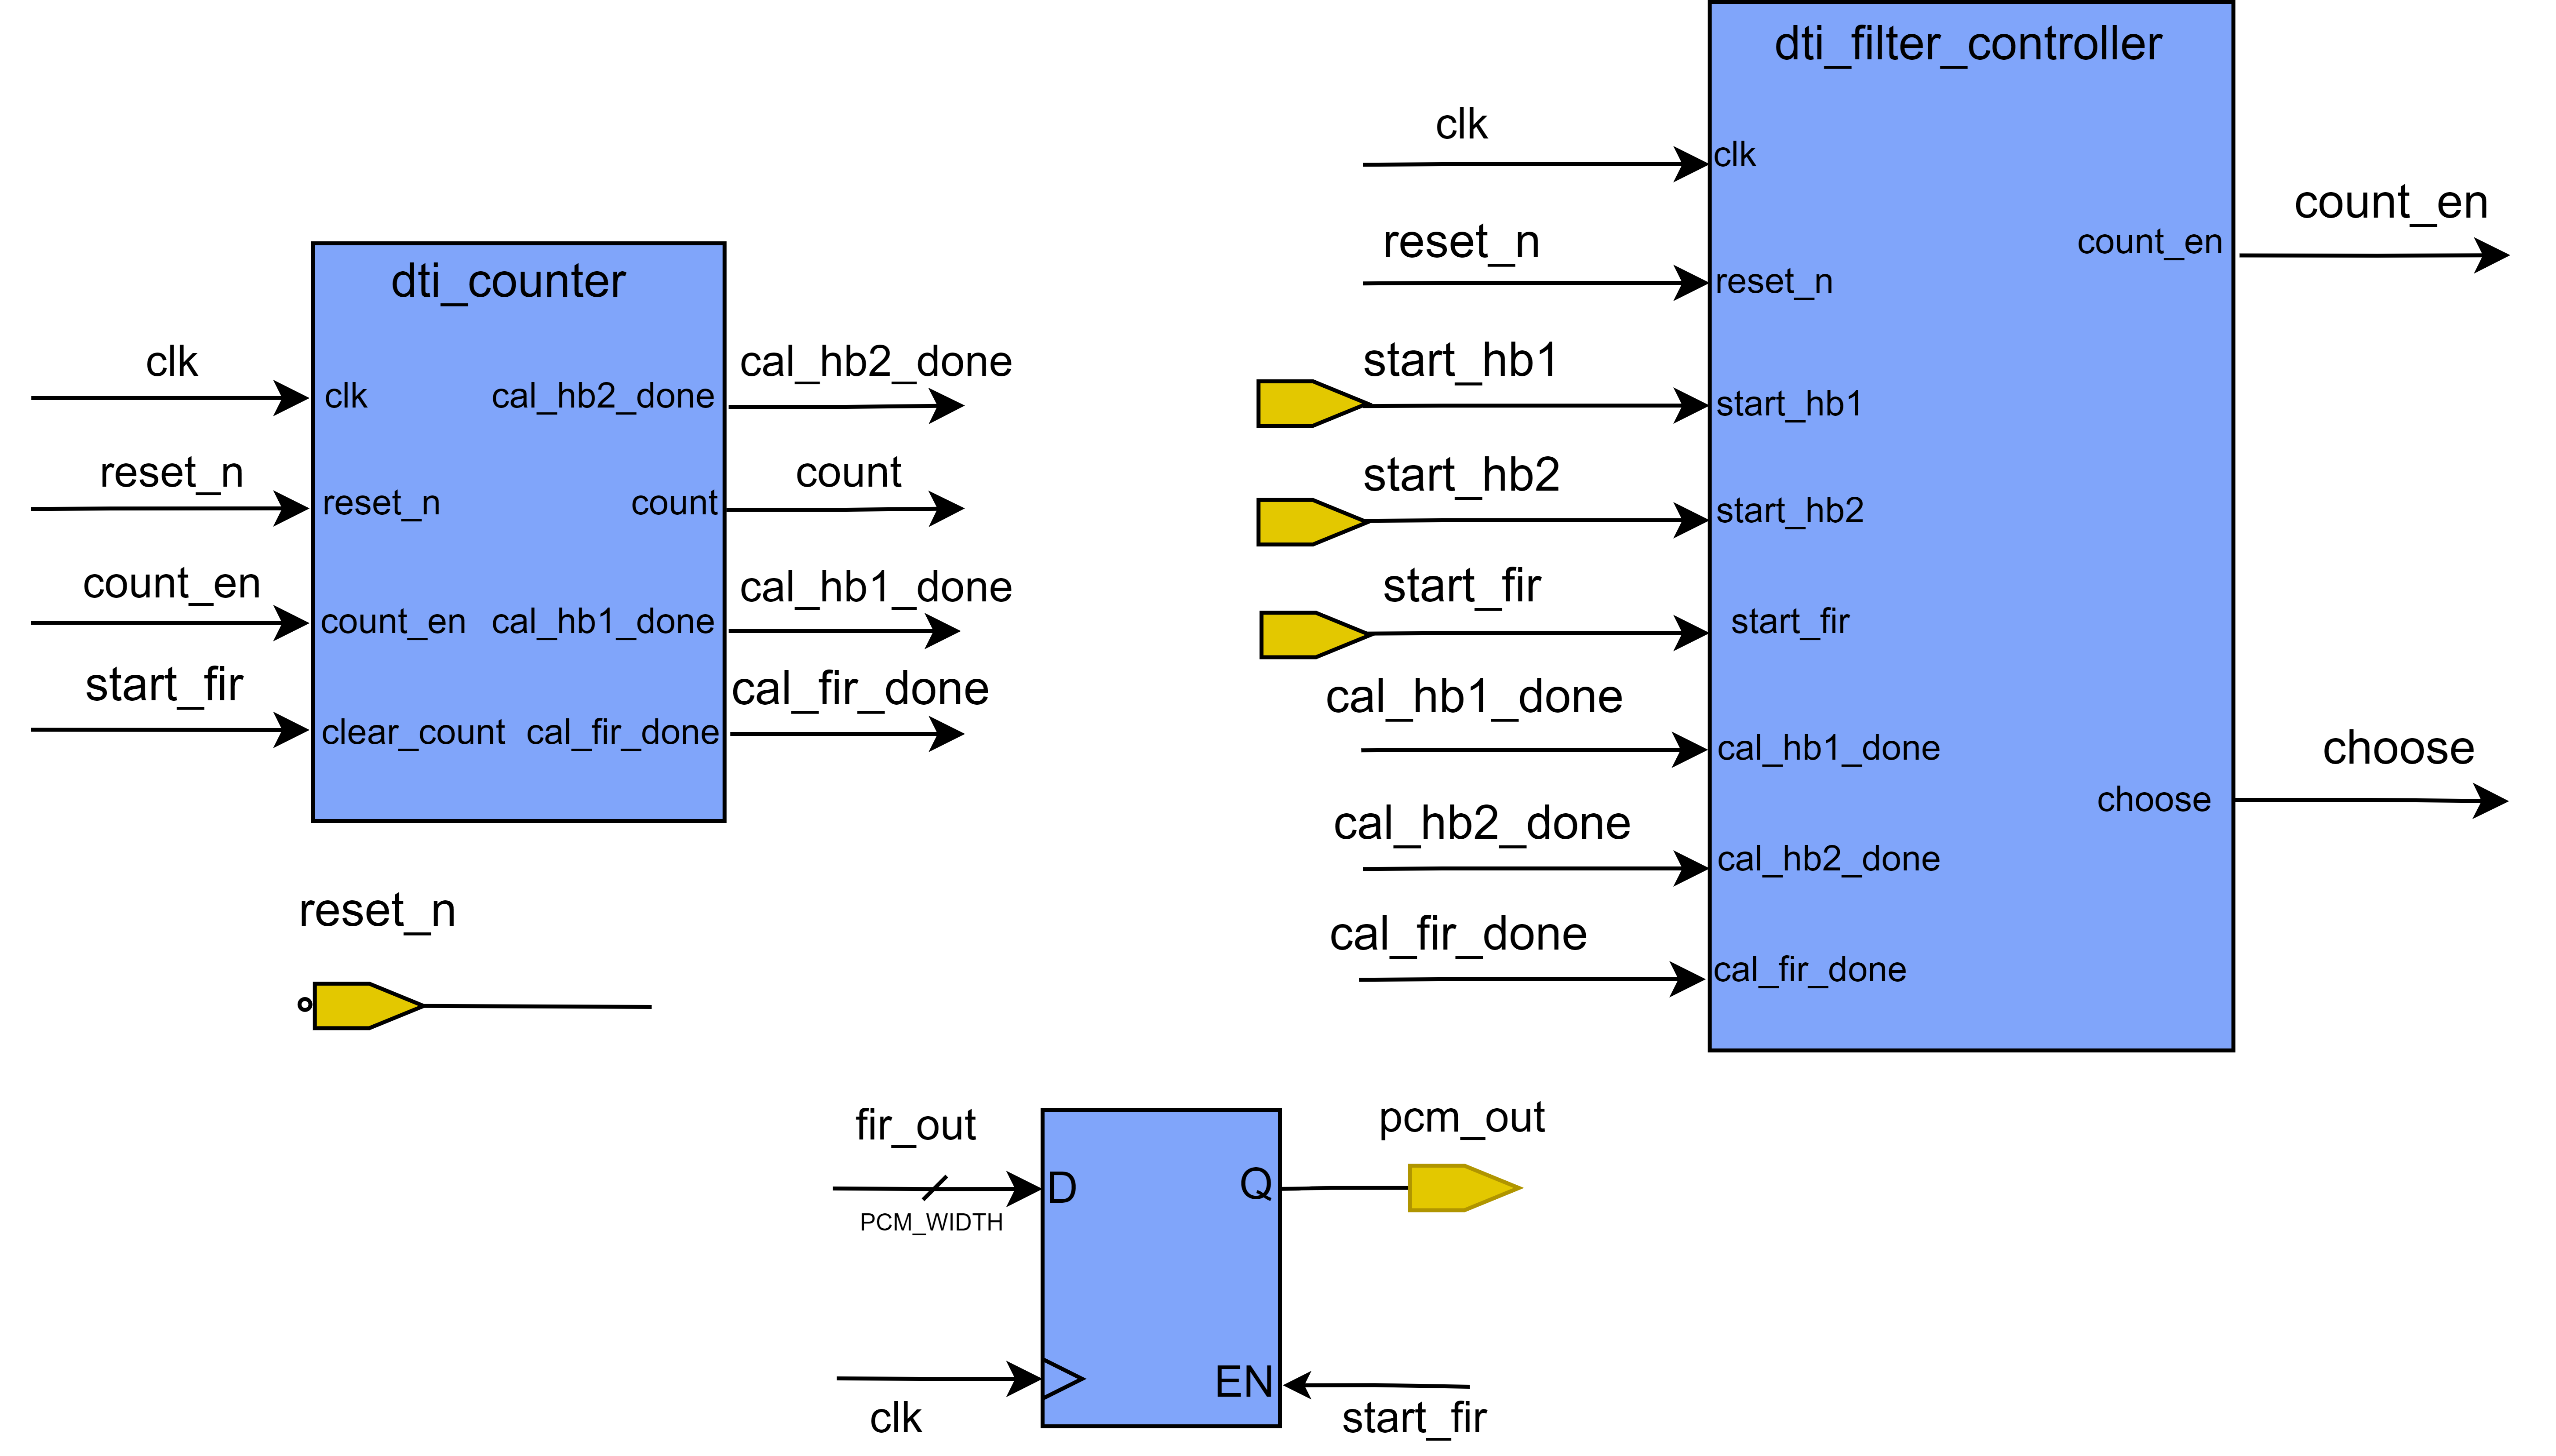
\includegraphics[width=13cm]{Images/Chuong4/hb_fir/fir.png}
    \caption[Kiến trúc các khối điều khiển trong dti\_hb\_fir\_filter]{\bfseries \fontsize{12pt}{0pt}\selectfont Kiến trúc các khối điều khiển trong dti\_hb\_fir\_filter}
    \label{control}
\end{figure}

Hình \ref{pre} và hình \ref{pos} mô tả kiến trúc của phần trước và sau của bộc lọc FIR. Chúng ta có thể thấy chỉ sử dụng 2 bộ cộng - 1 cộng cho các phần tử đối xứng và 1 để cộng dồn các phép toán nhân. Với 2 bộ lọc HB1 và HB2 còn lại sẽ thực hiện tương tự.

Bộ nhân sử dụng ở đây là bộ nhân Booth Wallace, nó là IP số có sẵn của công ty \textbf{Dolphin Technology Việt Nam}.

Với kiến trúc của bộ nhân chung (hình \ref{c_mul}), chúng ta sẽ duyệt các hệ số của các taps sau đó tiến hành nhân ở các thời điểm nhất định. Các hệ số sẽ được lưu ở bộ \textbf{coeff\_lut}, nó được xem là 1 bộ mem, các hệ số sẽ được lưu thứ tự FIR - HB1 - HB2 - HB1 (từ 0 đến 39). Dữ liệu sẽ đưa đưa ra theo địa chỉ \textit{count} tương ứng. Bảng \ref{coeffff} mô tả trình tự sắp đặt dữ liệu trong khối \textbf{coeff\_lut}.

\textbf{dti\_count} hoạt động như một trình tạo địa chỉ và bộ điều khiển của \textbf{dti\_filter\_controller}. Giá trị đếm dùng để chọn hệ số trong bảng tra cứu hệ số bộ lọc (\textbf{dti\_coeff\_lut}).

\paragraph{dti\_filter\_controller}
\begin{figure}[H]
    \centering
    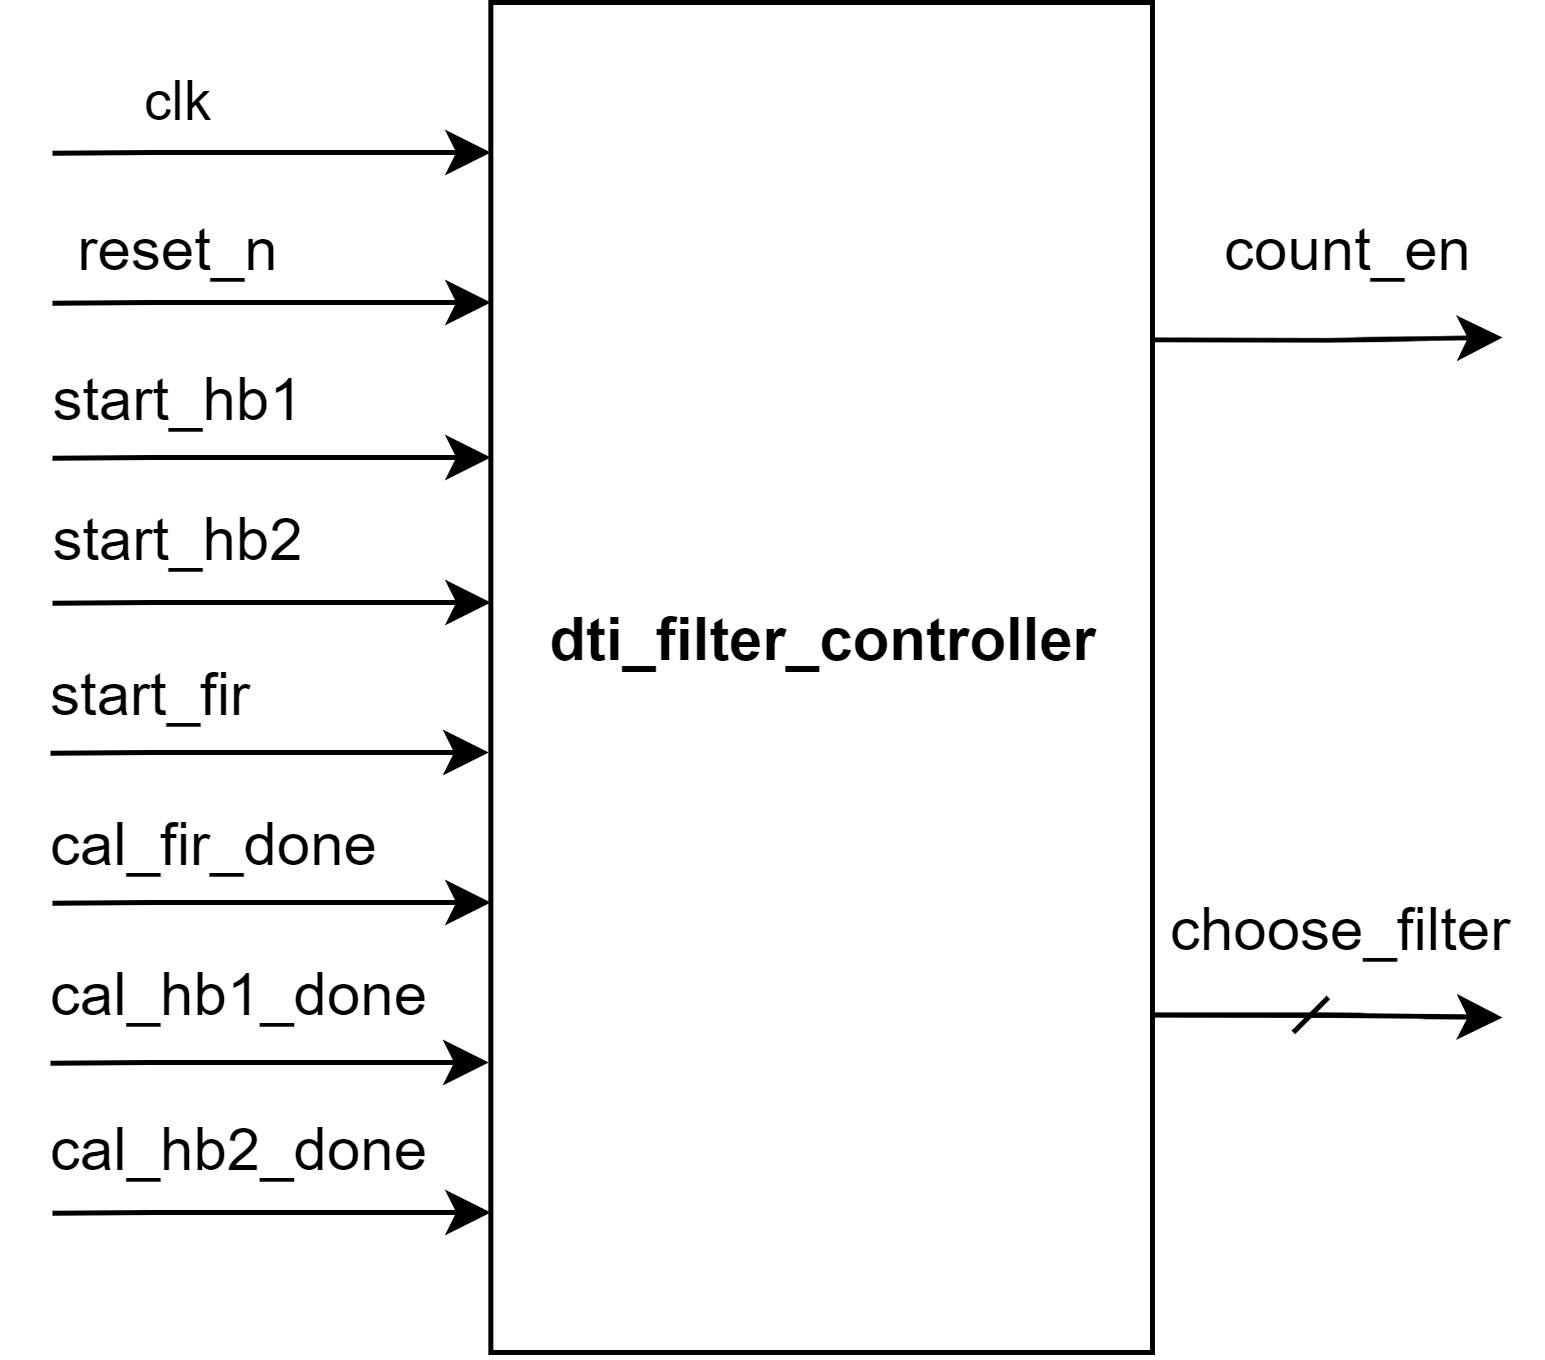
\includegraphics[width=6cm]{Images/Chuong4/hb_fir/control-top.png}
    \caption[Sơ đồ khối của dti\_filter\_controller]{\bfseries \fontsize{12pt}{0pt}\selectfont Sơ đồ khối của dti\_filter\_controller}
    \label{control_t}
\end{figure}
\textbf{dti\_hb\_fir\_filter} chỉ sử dụng 1 bộ nhân nên 2 bộ lọc Half band và bộ lọc FIR buộc phải chia sẻ tài nguyên. \textbf{dti\_filter\_controller} kiểm soát việc sử dụng tài nguyên của các bộ lọc bằng tín hiệu \textbf{select\_filter}.

\begin{figure}[H]
    \centering
    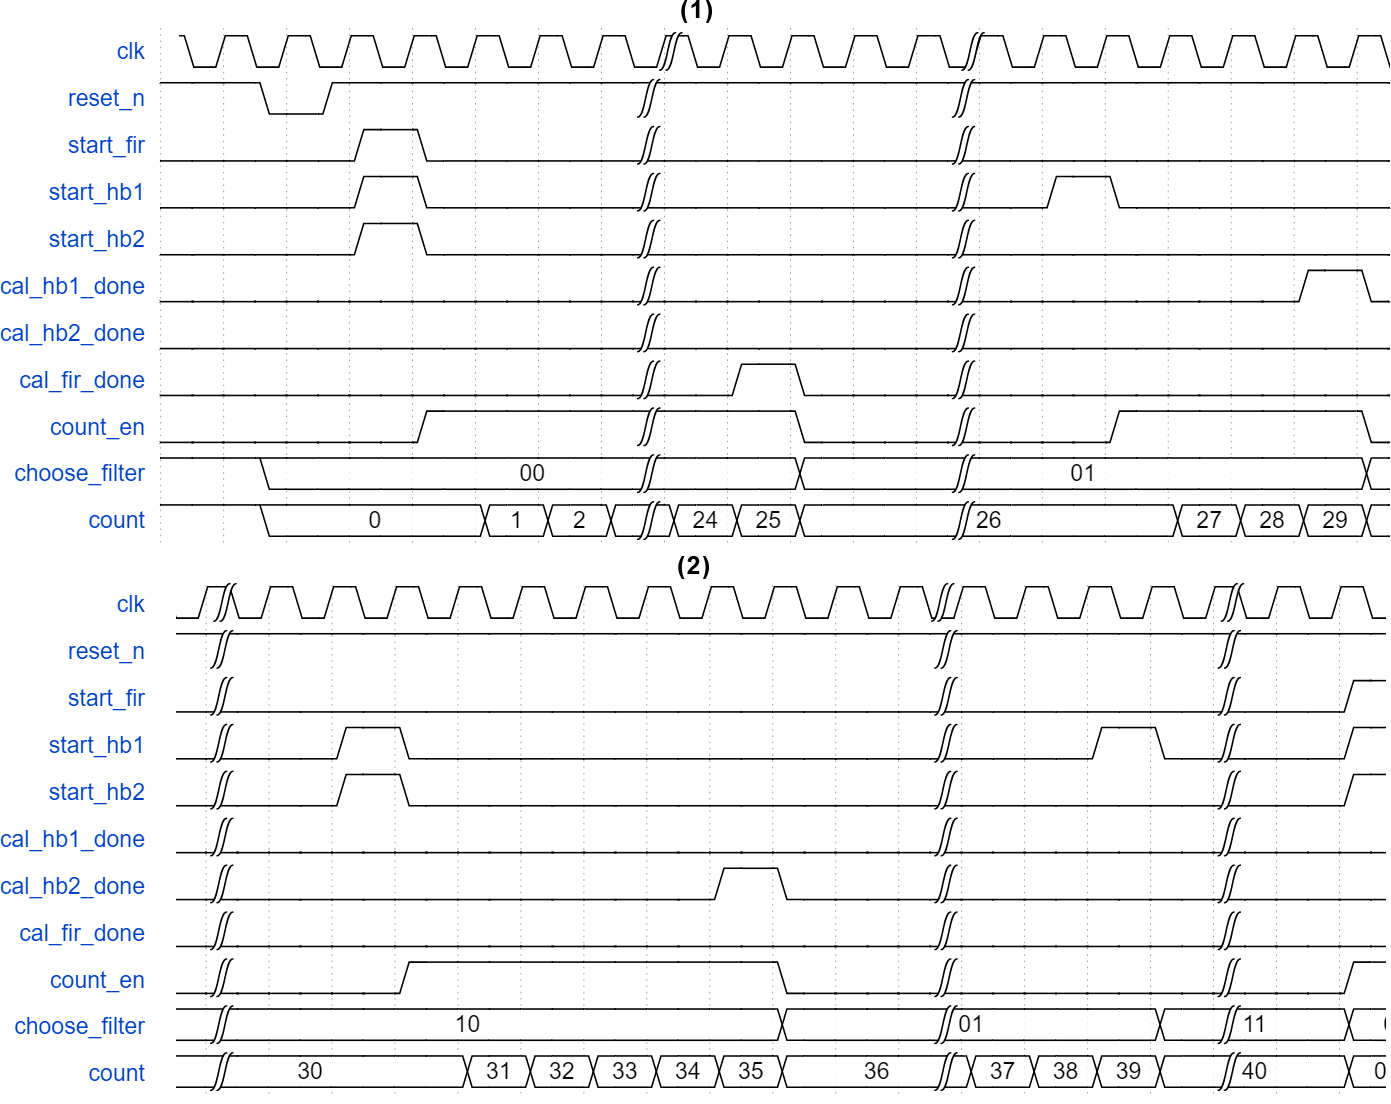
\includegraphics[width=13cm]{Images/Chuong4/hb_fir/control-timing.png}
    \caption[Biểu đồ thời của dti\_filter\_controller]{\bfseries \fontsize{12pt}{0pt}\selectfont Biểu đồ thời  của dti\_filter\_controller}
    \label{control_timing}
\end{figure}
\begin{figure}[H]
    \centering
    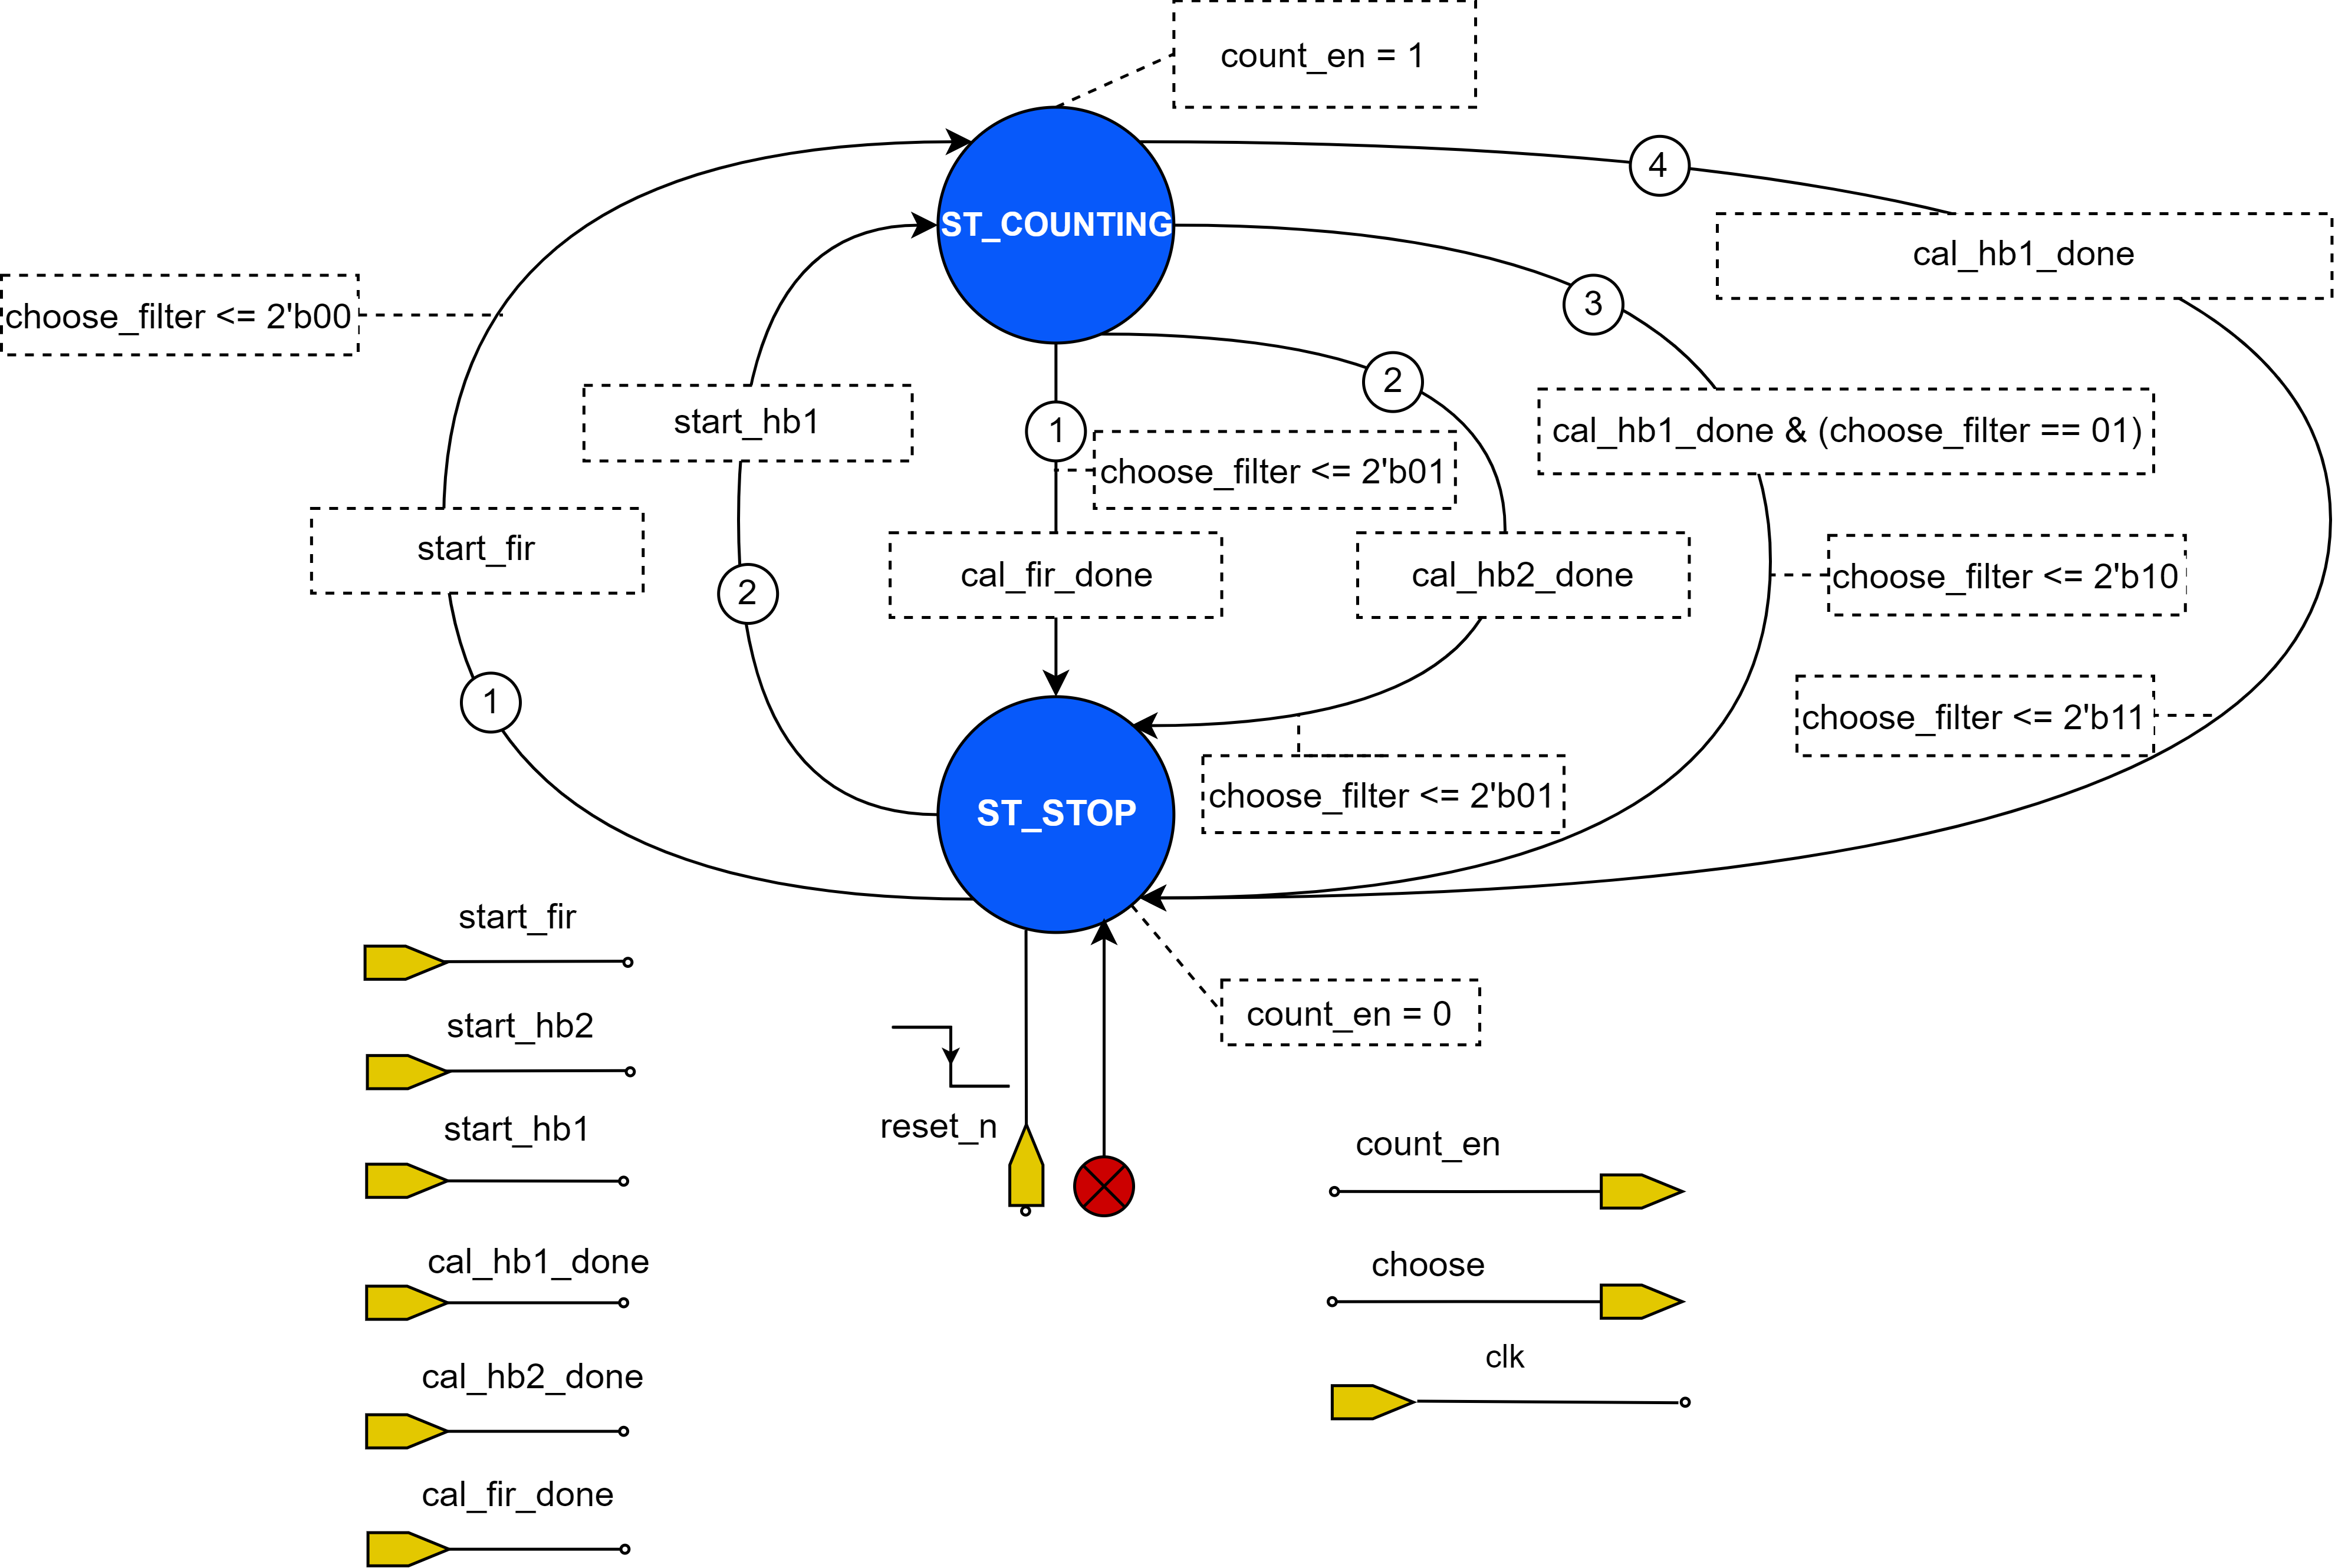
\includegraphics[width=14cm]{Images/Chuong4/hb_fir/control-fsm.png}
    \caption[Sơ đồ máy trạng thái hữu hạn của dti\_filter\_controller]{\bfseries \fontsize{12pt}{0pt}\selectfont Sơ đồ máy trạng thái hữu hạn của dti\_filter\_controller}
    \label{control_fsm}
\end{figure}
Sơ đồ chân vào ra mô tả ở hình \ref{control_t}. Các tín hiệu điều khiển hoạt động với chức năng thể hiện ở biểu đồ hình \ref{control_timing}.

Qua sơ đồ hình \ref{control_fsm}, máy trạng thái của bộ có 2 trạng thái:
\begin{itemize}
    \item \textbf{ST\_COUNTING}: bộ đếm tăng giá trị
    \item \textbf{ST\_STOP}: bộ đếm dừng hoạt động
\end{itemize}

Bộ điều khiển có chức năng chia pha cho và chọn thời điểm lấy giá trị đưa vào bộ nhân. Nó cũng điều khiển bộ đếm để lấy giá trị các hệ số của các bộ lọc trong MEM ra. Việc kích hoạt từng bộ lọc sẽ được điều khiển bởi tín hiệu choose\_filter. Vì tần số hệ thống lớn hơn rất nhiều so với điều kiện trong 1 chu kỳ thực hiện phép nhân nên bộ điều khiển phải lấy tín hiệu thực hiện xong tính toán của từng bộ lọc để chờ ở các pha tính toán tiếp theo. 

\begin{table}[H]
\centering
    \caption[Các hệ số của các bộ lọc ứng với từng địa chỉ trong khối coeff\_lut]{\bfseries \fontsize{12pt}{0pt}\selectfont Các hệ số của các bộ lọc ứng với từng địa chỉ trong khối coeff\_lut}
\begin{tabular}{|l|c|c|l|l|c|c|}
\cline{1-3} \cline{5-7}
\multicolumn{1}{|c|}{\textbf{Địa chỉ}} & \textbf{Bộ lọc}       & \textbf{Giá trị} &  & \multicolumn{1}{c|}{\textbf{Địa chỉ}} & \textbf{Bộ lọc}       & \textbf{Giá trị} \\ \cline{1-3} \cline{5-7} 
0                                      & \multirow{10}{*}{FIR} & -96              &  & 10                                    & \multirow{10}{*}{FIR} & 5333             \\ \cline{1-1} \cline{3-3} \cline{5-5} \cline{7-7} 
1 &  & -191  &  & 11 &  & 8971   \\ \cline{1-1} \cline{3-3} \cline{5-5} \cline{7-7} 
2 &  & -12   &  & 12 &  & 4117   \\ \cline{1-1} \cline{3-3} \cline{5-5} \cline{7-7} 
3 &  & 683   &  & 13 &  & -8082  \\ \cline{1-1} \cline{3-3} \cline{5-5} \cline{7-7} 
4 &  & 1560  &  & 14 &  & -17116 \\ \cline{1-1} \cline{3-3} \cline{5-5} \cline{7-7} 
5 &  & 1559  &  & 15 &  & -10866 \\ \cline{1-1} \cline{3-3} \cline{5-5} \cline{7-7} 
6 &  & -220  &  & 16 &  & 10947  \\ \cline{1-1} \cline{3-3} \cline{5-5} \cline{7-7} 
7 &  & -3024 &  & 17 &  & 30749  \\ \cline{1-1} \cline{3-3} \cline{5-5} \cline{7-7} 
8 &  & -4108 &  & 18 &  & 24711  \\ \cline{1-1} \cline{3-3} \cline{5-5} \cline{7-7} 
9 &  & -938  &  & 19 &  & -13469 \\ \cline{1-3} \cline{5-7} 
\end{tabular}
\label{coeffff}
\end{table}
\begin{table}[H]
\centering
\begin{tabular}{|l|c|c|l|l|c|c|}
\cline{1-3} \cline{5-7}
\multicolumn{1}{|c|}{\textbf{Địa chỉ}} & \textbf{Bộ lọc} & \textbf{Giá trị} &  & \multicolumn{1}{c|}{\textbf{Địa chỉ}} & \textbf{Bộ lọc} & \textbf{Giá trị} \\ \cline{1-3} \cline{5-7} 
20 & \multirow{6}{*}{FIR} & -57165 &  & 30 & \multirow{6}{*}{HB2} & 749    \\ \cline{1-1} \cline{3-3} \cline{5-5} \cline{7-7} 
21 &                      & -58588 &  & 31 &                      & -5783  \\ \cline{1-1} \cline{3-3} \cline{5-5} \cline{7-7} 
22 &                      & 15205  &  & 32 &                      & 24260  \\ \cline{1-1} \cline{3-3} \cline{5-5} \cline{7-7} 
23 &                      & 149059 &  & 33 &                      & -78249 \\ \cline{1-1} \cline{3-3} \cline{5-5} \cline{7-7} 
24 &                      & 279548 &  & 34 &                      & 321172 \\ \cline{1-1} \cline{3-3} \cline{5-5} \cline{7-7} 
25 &                      & 333704 &  & 35 &                      & 524288 \\ \cline{1-3} \cline{5-7} 
26 & \multirow{4}{*}{HB1} & 7025   &  & 36 & \multirow{4}{*}{HB1} & 7025   \\ \cline{1-1} \cline{3-3} \cline{5-5} \cline{7-7} 
27 &                      & -53701 &  & 37 &                      & -53701 \\ \cline{1-1} \cline{3-3} \cline{5-5} \cline{7-7} 
28 &                      & 308825 &  & 38 &                      & 308825 \\ \cline{1-1} \cline{3-3} \cline{5-5} \cline{7-7} 
29 &                      & 524288 &  & 39 &                      & 524288 \\ \cline{1-3} \cline{5-7} 
\end{tabular}
\end{table}

\subsection{Kiểm thử}
Việc mô phỏng RTL sẽ được thực hiện trên Mentor Questasim. Tương tự chương 2, chúng ta sẽ trích xuất tín hiệu PDM từ bộ điều chế (thư viện sigmadelta) ra dữ liệu dạng chữ và lưu vào tệp text. Từ đó có thể đưa vào testbench và chạy mô phỏng.
\subsubsection{Cấu trúc testbench}
\begin{figure}[H]
    \centering
    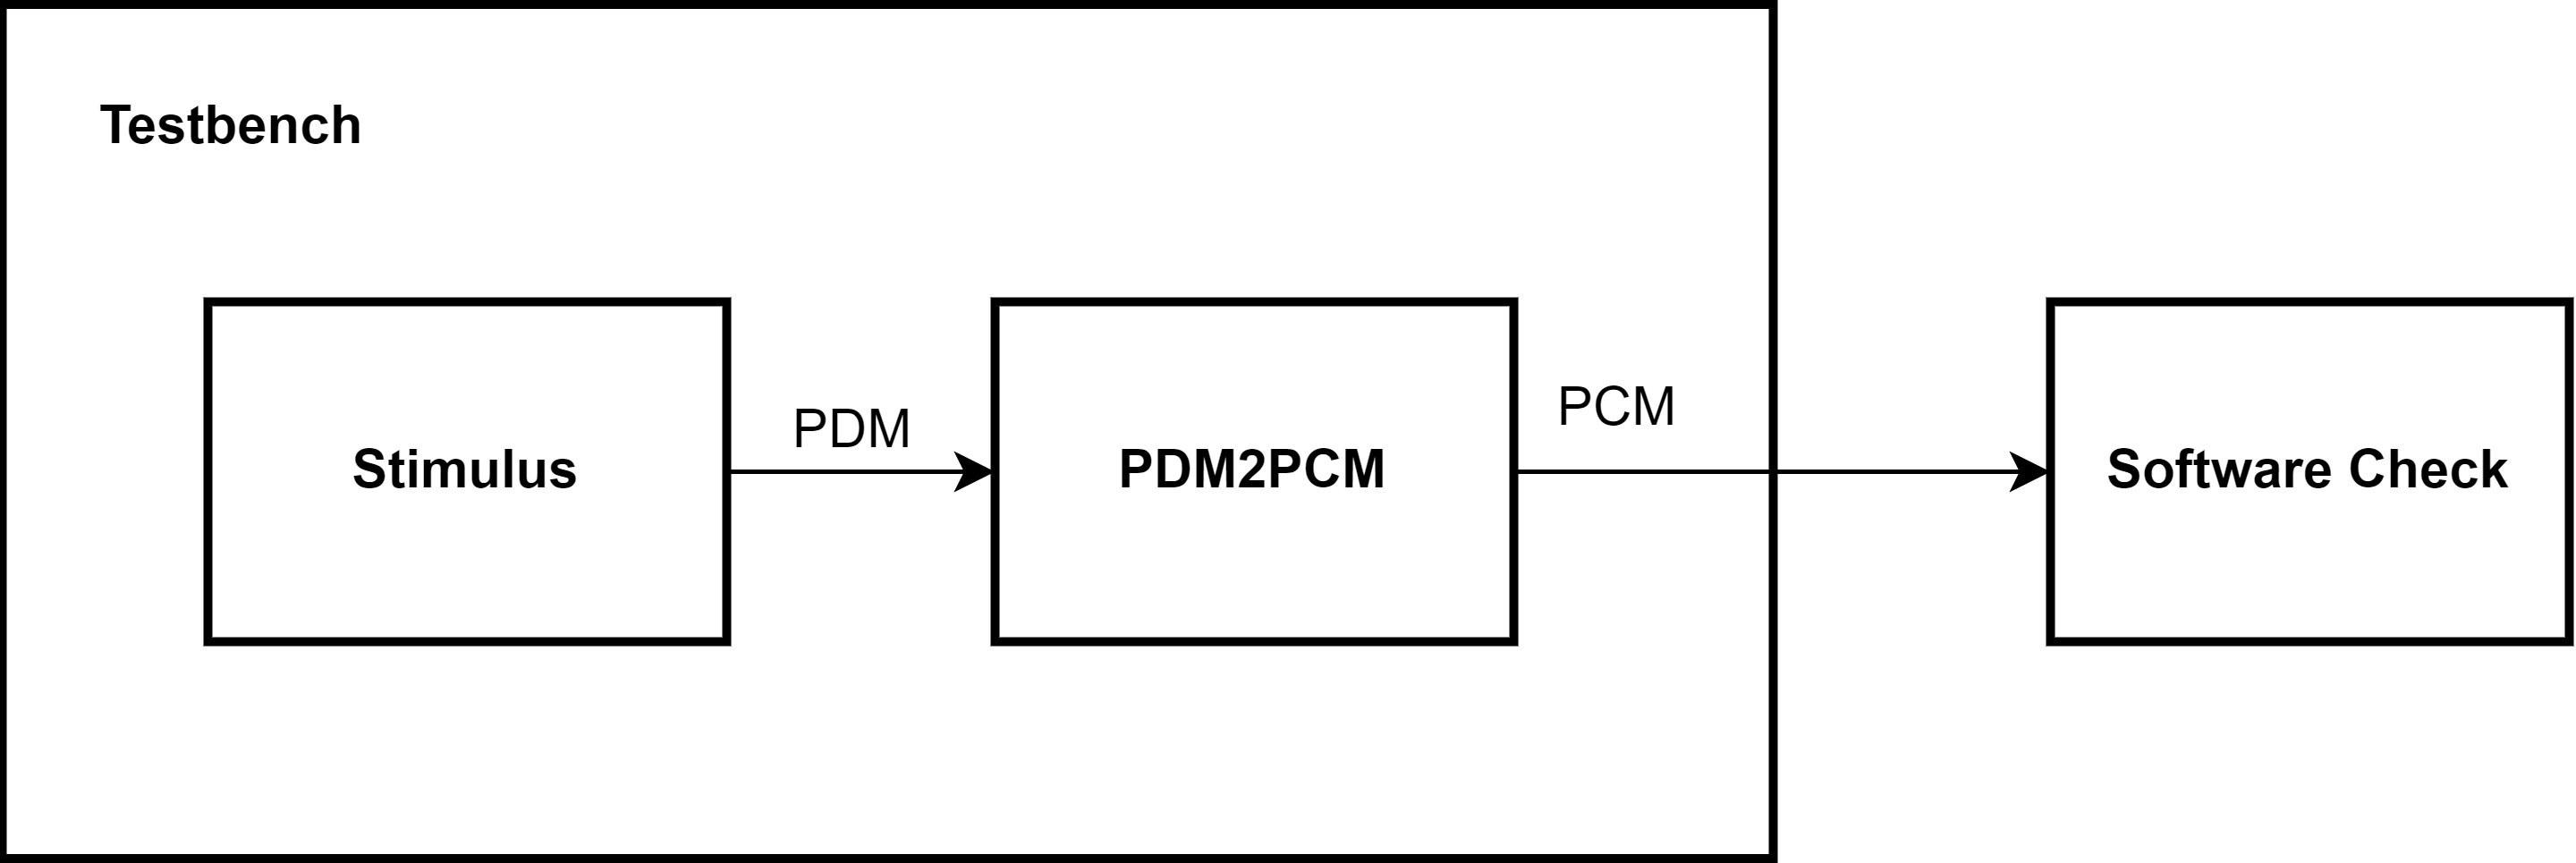
\includegraphics[width=13cm]{Images/Chuong4/tb/tb_top.png}
    \caption[Cấu trúc của testbench]{\bfseries \fontsize{12pt}{0pt}\selectfont  Cấu trúc của testbench}
    \label{tb_top}
\end{figure}

Tín hiệu PDM được đọc từ tệp text thu được bộ điều chế đưa vào thiết kế với tần số lấy mẫu của PDM (2304 kHz). Dữ liệu PCM thu được đầu ra với tần số mẫu là 48 kHz đưa ghi vào tệp text. Từ tệp đó chúng ta sẽ so sánh với kết quả tính toán bằng phần mềm sử dụng ngôn ngữ \textbf{python} (hình \ref{tb_top}). Việc so sánh sẽ đựa vào biểu đồ mật độ phổ công suất và tín hiệu ở miền thời gian.

\subsubsection{Kết quả mô phỏng}
\paragraph{Tín hiệu nhiều thành phần sin}
Như ở trong \hyperref[chuong3]{chương 3}, tín hiệu đầu vào chứa các thành phần gồm các sóng sin trong dải tần từ 0 - 24 kHz, mỗi thành phần tần số sẽ cách nhau 0.01 kHz và được biểu diễn như phương trình \ref{3sins}.
\begin{equation} \label{3sins}
    x(t) = \frac{0.5}{2400}\sum^{2400}_{f = 1}sin(2\pi \times 100 \times f \times t)
\end{equation}

Do bộ lọc trên phần mềm đã được kiểm chứng ở chương 3 cho nên bây giờ chúng ta sẽ so sánh tín hiệu đầu ra của phần cứng so với phần mềm để đưa ra kết luận.


Hình \ref{sin_1} và \ref{sin_1_h} miêu tả biểu đồ thời gian của tín hiệu PCM sau mô phỏng của cả phần cứng và phần mềm. Ở miền này chúng ta không thể nhận ra sự khác biệt giữa 2 tín hiệu. Vì vậy, để kết luận một cách rõ ràng hơn, chúng sẽ xem xét miền tần số của 2 tín hiệu. Hình \ref{sin_1_psd}, hình \ref{sin_1_psd_h} mô tả biểu đồ phổ mật độ công suất của 2 tín hiệu trên.

Ta thấy, các điểm tần số chuyển tiếp giữa các vùng (dải thông, dải chuyển tiếp, dải dừng) giữa 2 tín hiệu là giống giống nhau. Tuy nhiên, khi chúng ta tập trung vào dải dừng, với phần mềm độ suy hao ở dải đó cao nhất là 146.721 dB, còn phần cứng là 134.789, chênh lệch nhau 11.932 dB. 

\begin{figure}[H]
    \centering
    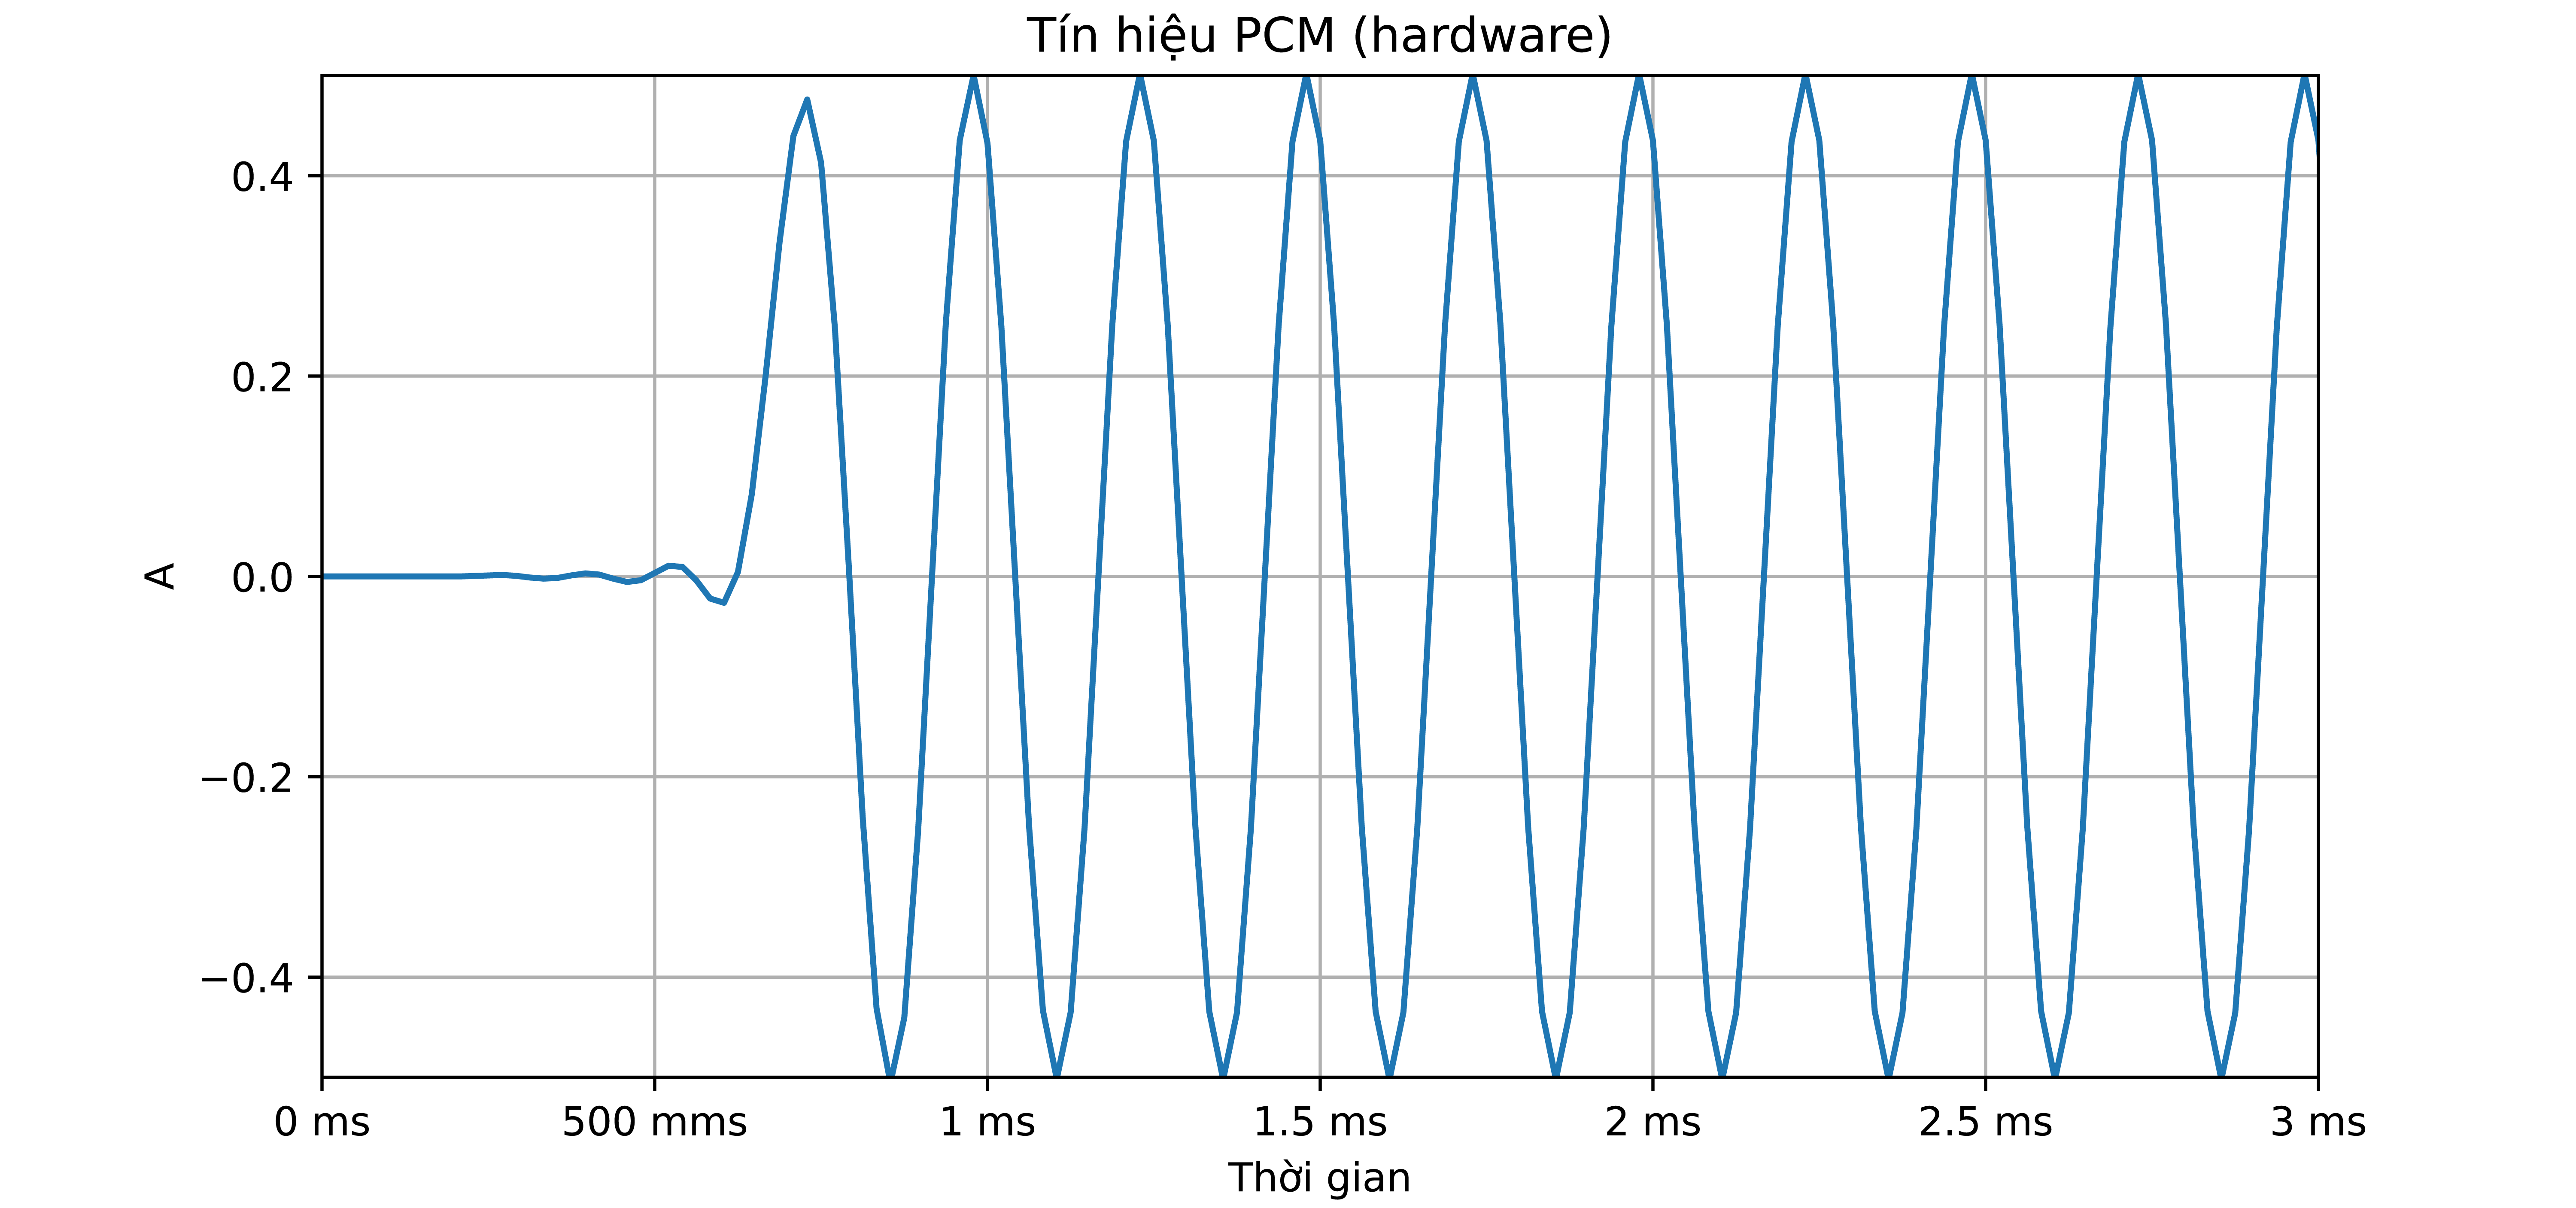
\includegraphics[width=12cm]{Images/Chuong4/tb/sim/sin_1.png}
    \caption[Miền thời gian của tín hiệu mô phỏng bằng phần mềm]{\bfseries \fontsize{12pt}{0pt}\selectfont Miền thời gian của tín hiệu mô phỏng bằng phần mềm}
    \label{sin_1}
\end{figure}

\begin{figure}[H]
    \centering
    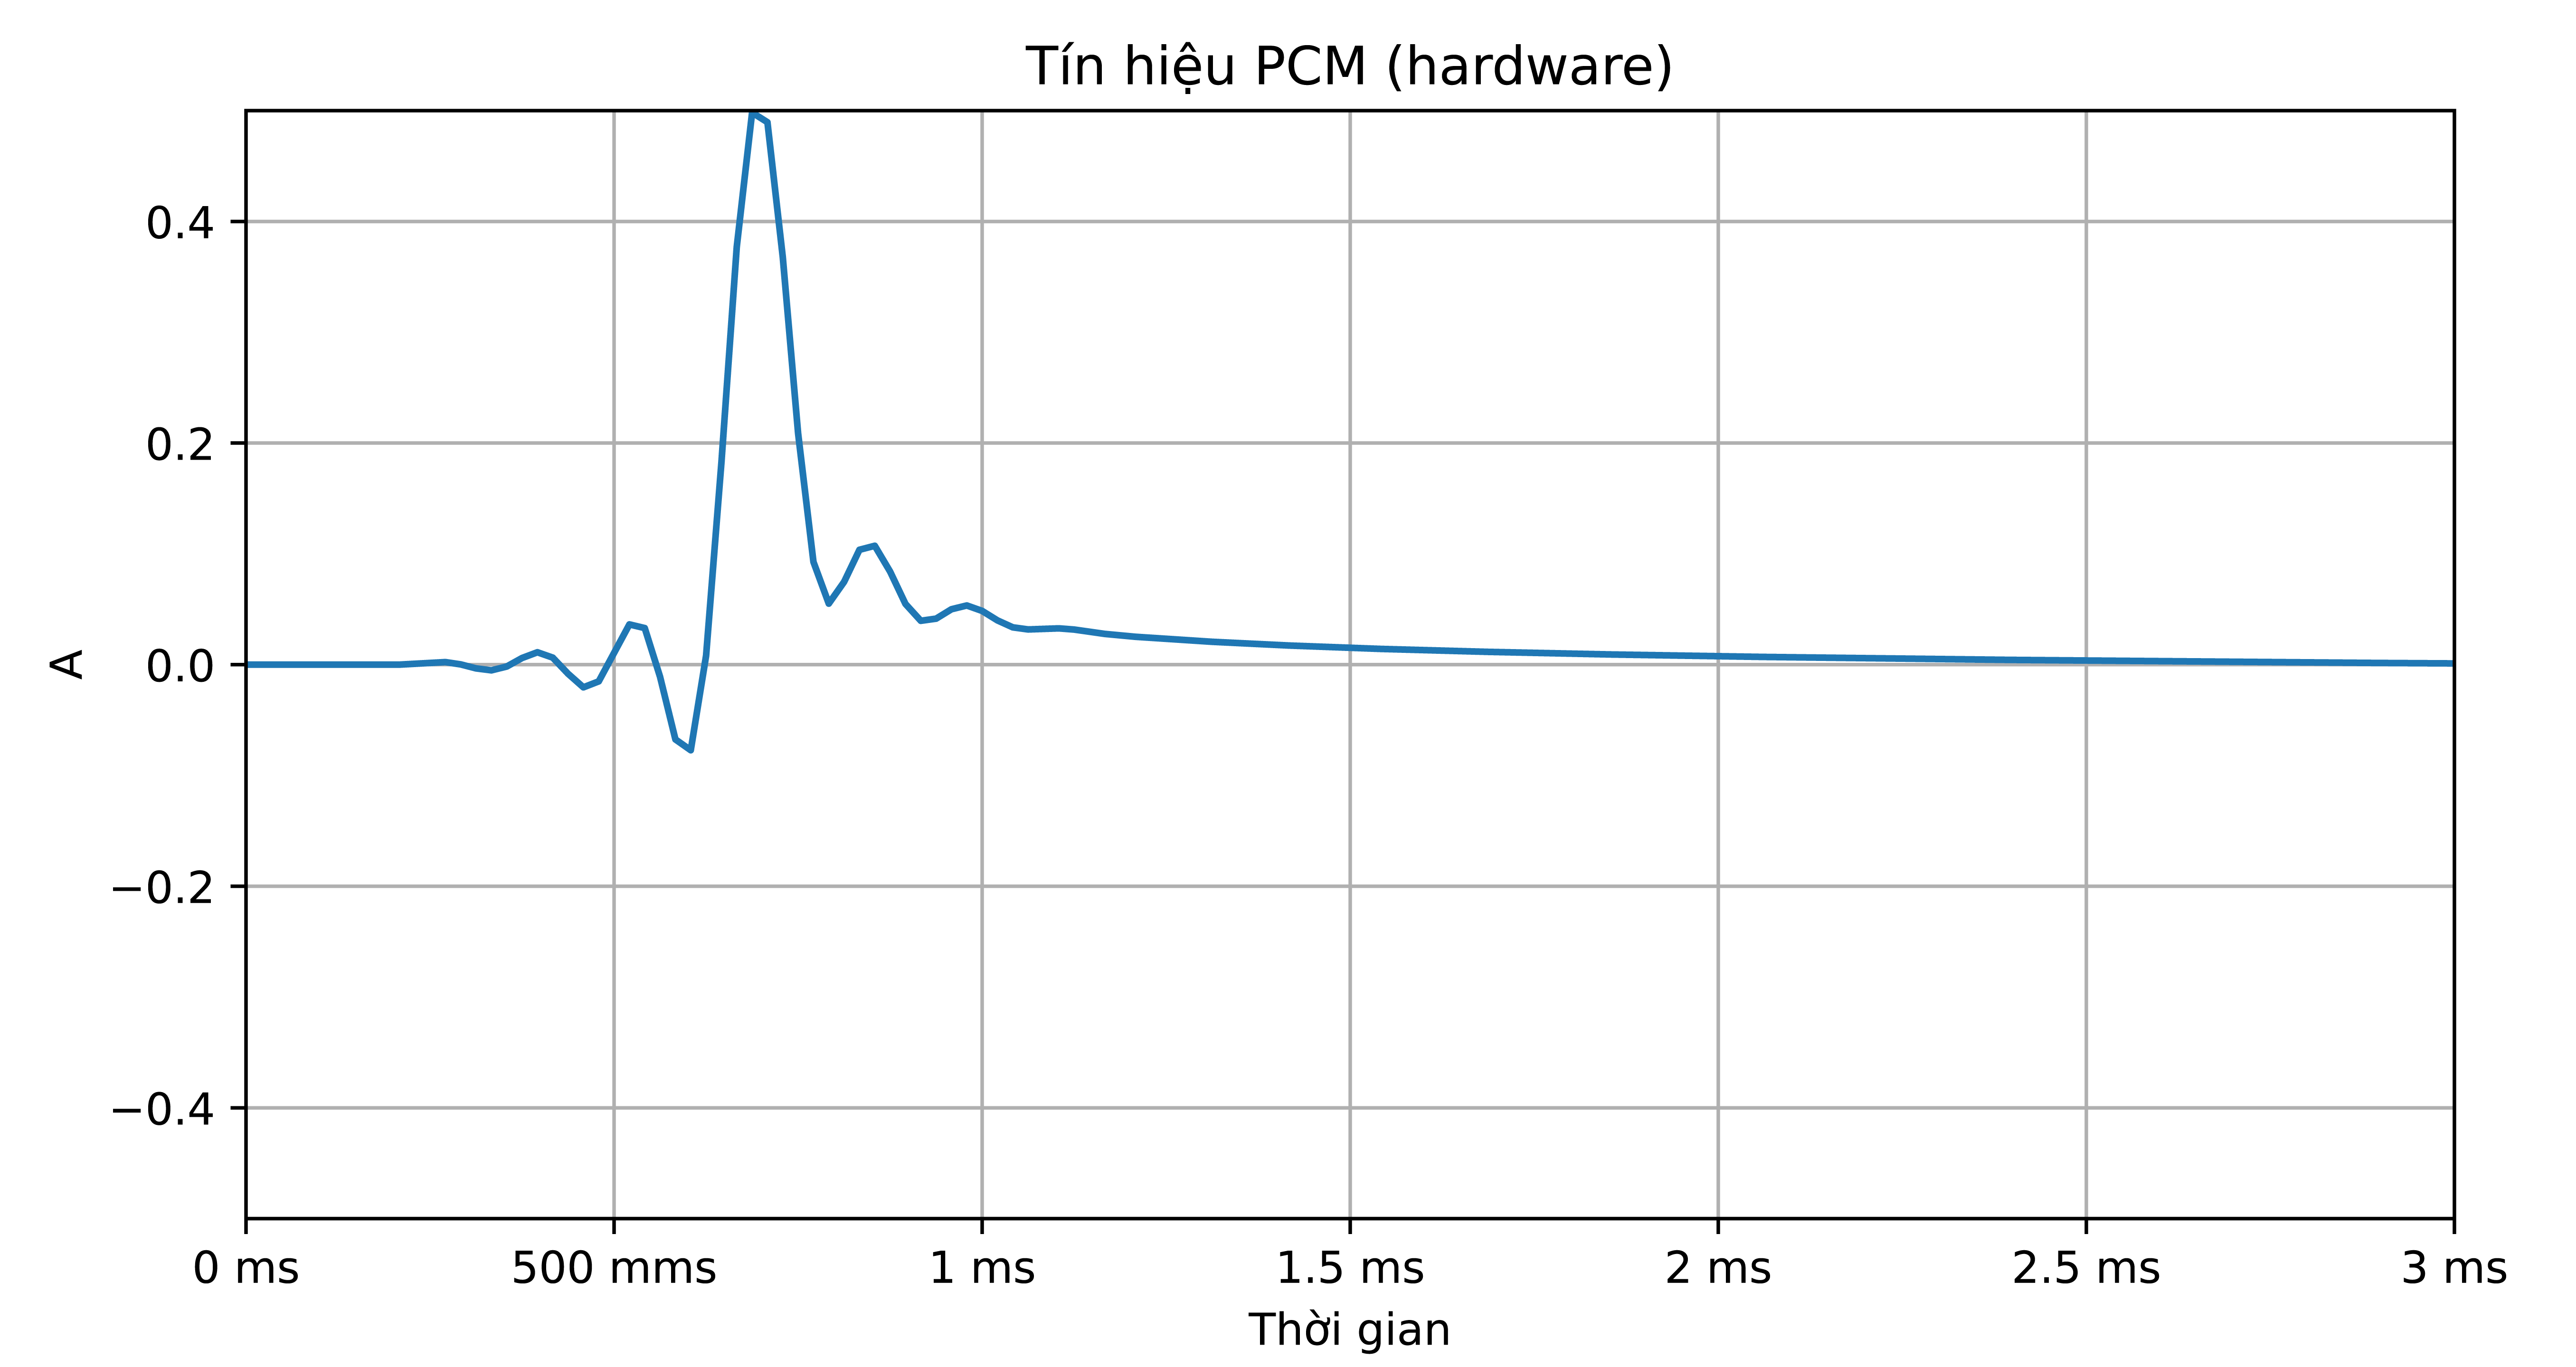
\includegraphics[width=12cm]{Images/Chuong4/tb/sim/sin_1_h.png}
    \caption[Miền thời gian của tín hiệu mô phỏng bằng phần cứng]{\bfseries \fontsize{12pt}{0pt}\selectfont Miền thời gian của tín hiệu mô phỏng bằng phần cứng}
    \label{sin_1_h}
\end{figure}

\begin{figure}[H]
    \centering
    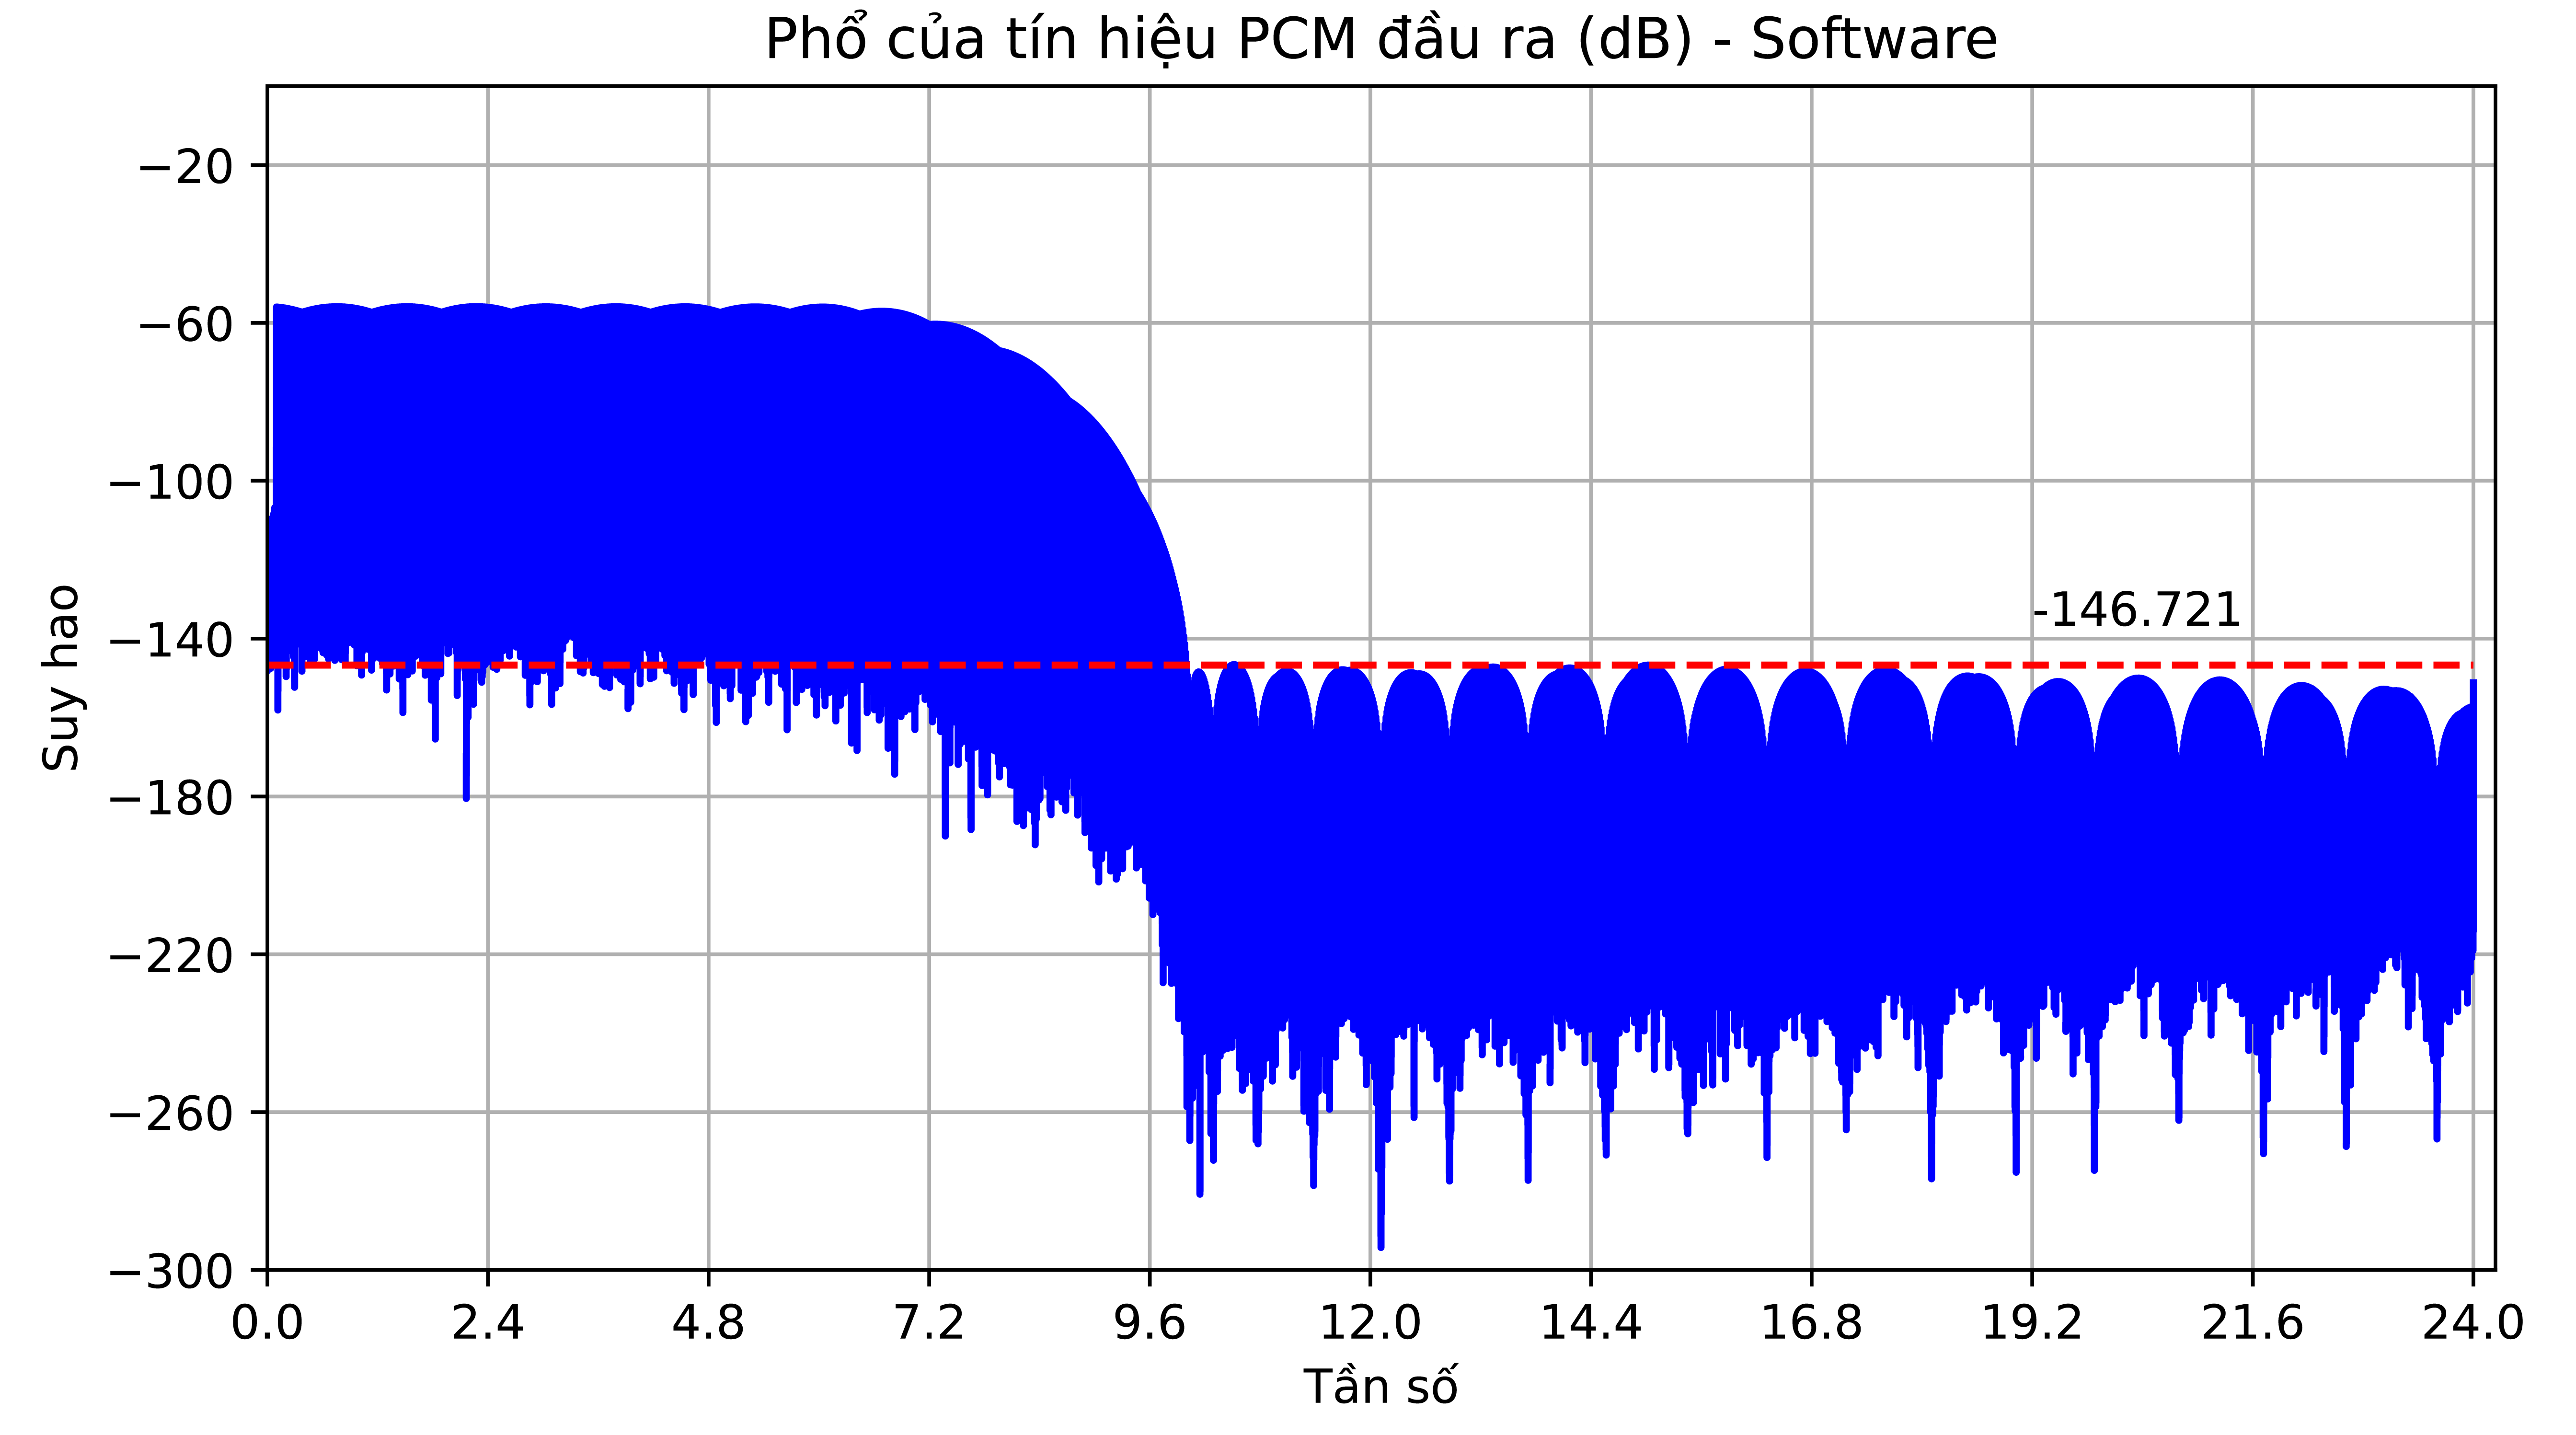
\includegraphics[width=12cm]{Images/Chuong4/tb/sim/sin_1_psd.png}
    \caption[Miền thời gian của tín hiệu mô phỏng bằng phần cứng]{\bfseries \fontsize{12pt}{0pt}\selectfont Miền thời gian của tín hiệu mô phỏng bằng phần cứng}
    \label{sin_1_psd}
\end{figure}

\begin{figure}[H]
    \centering
    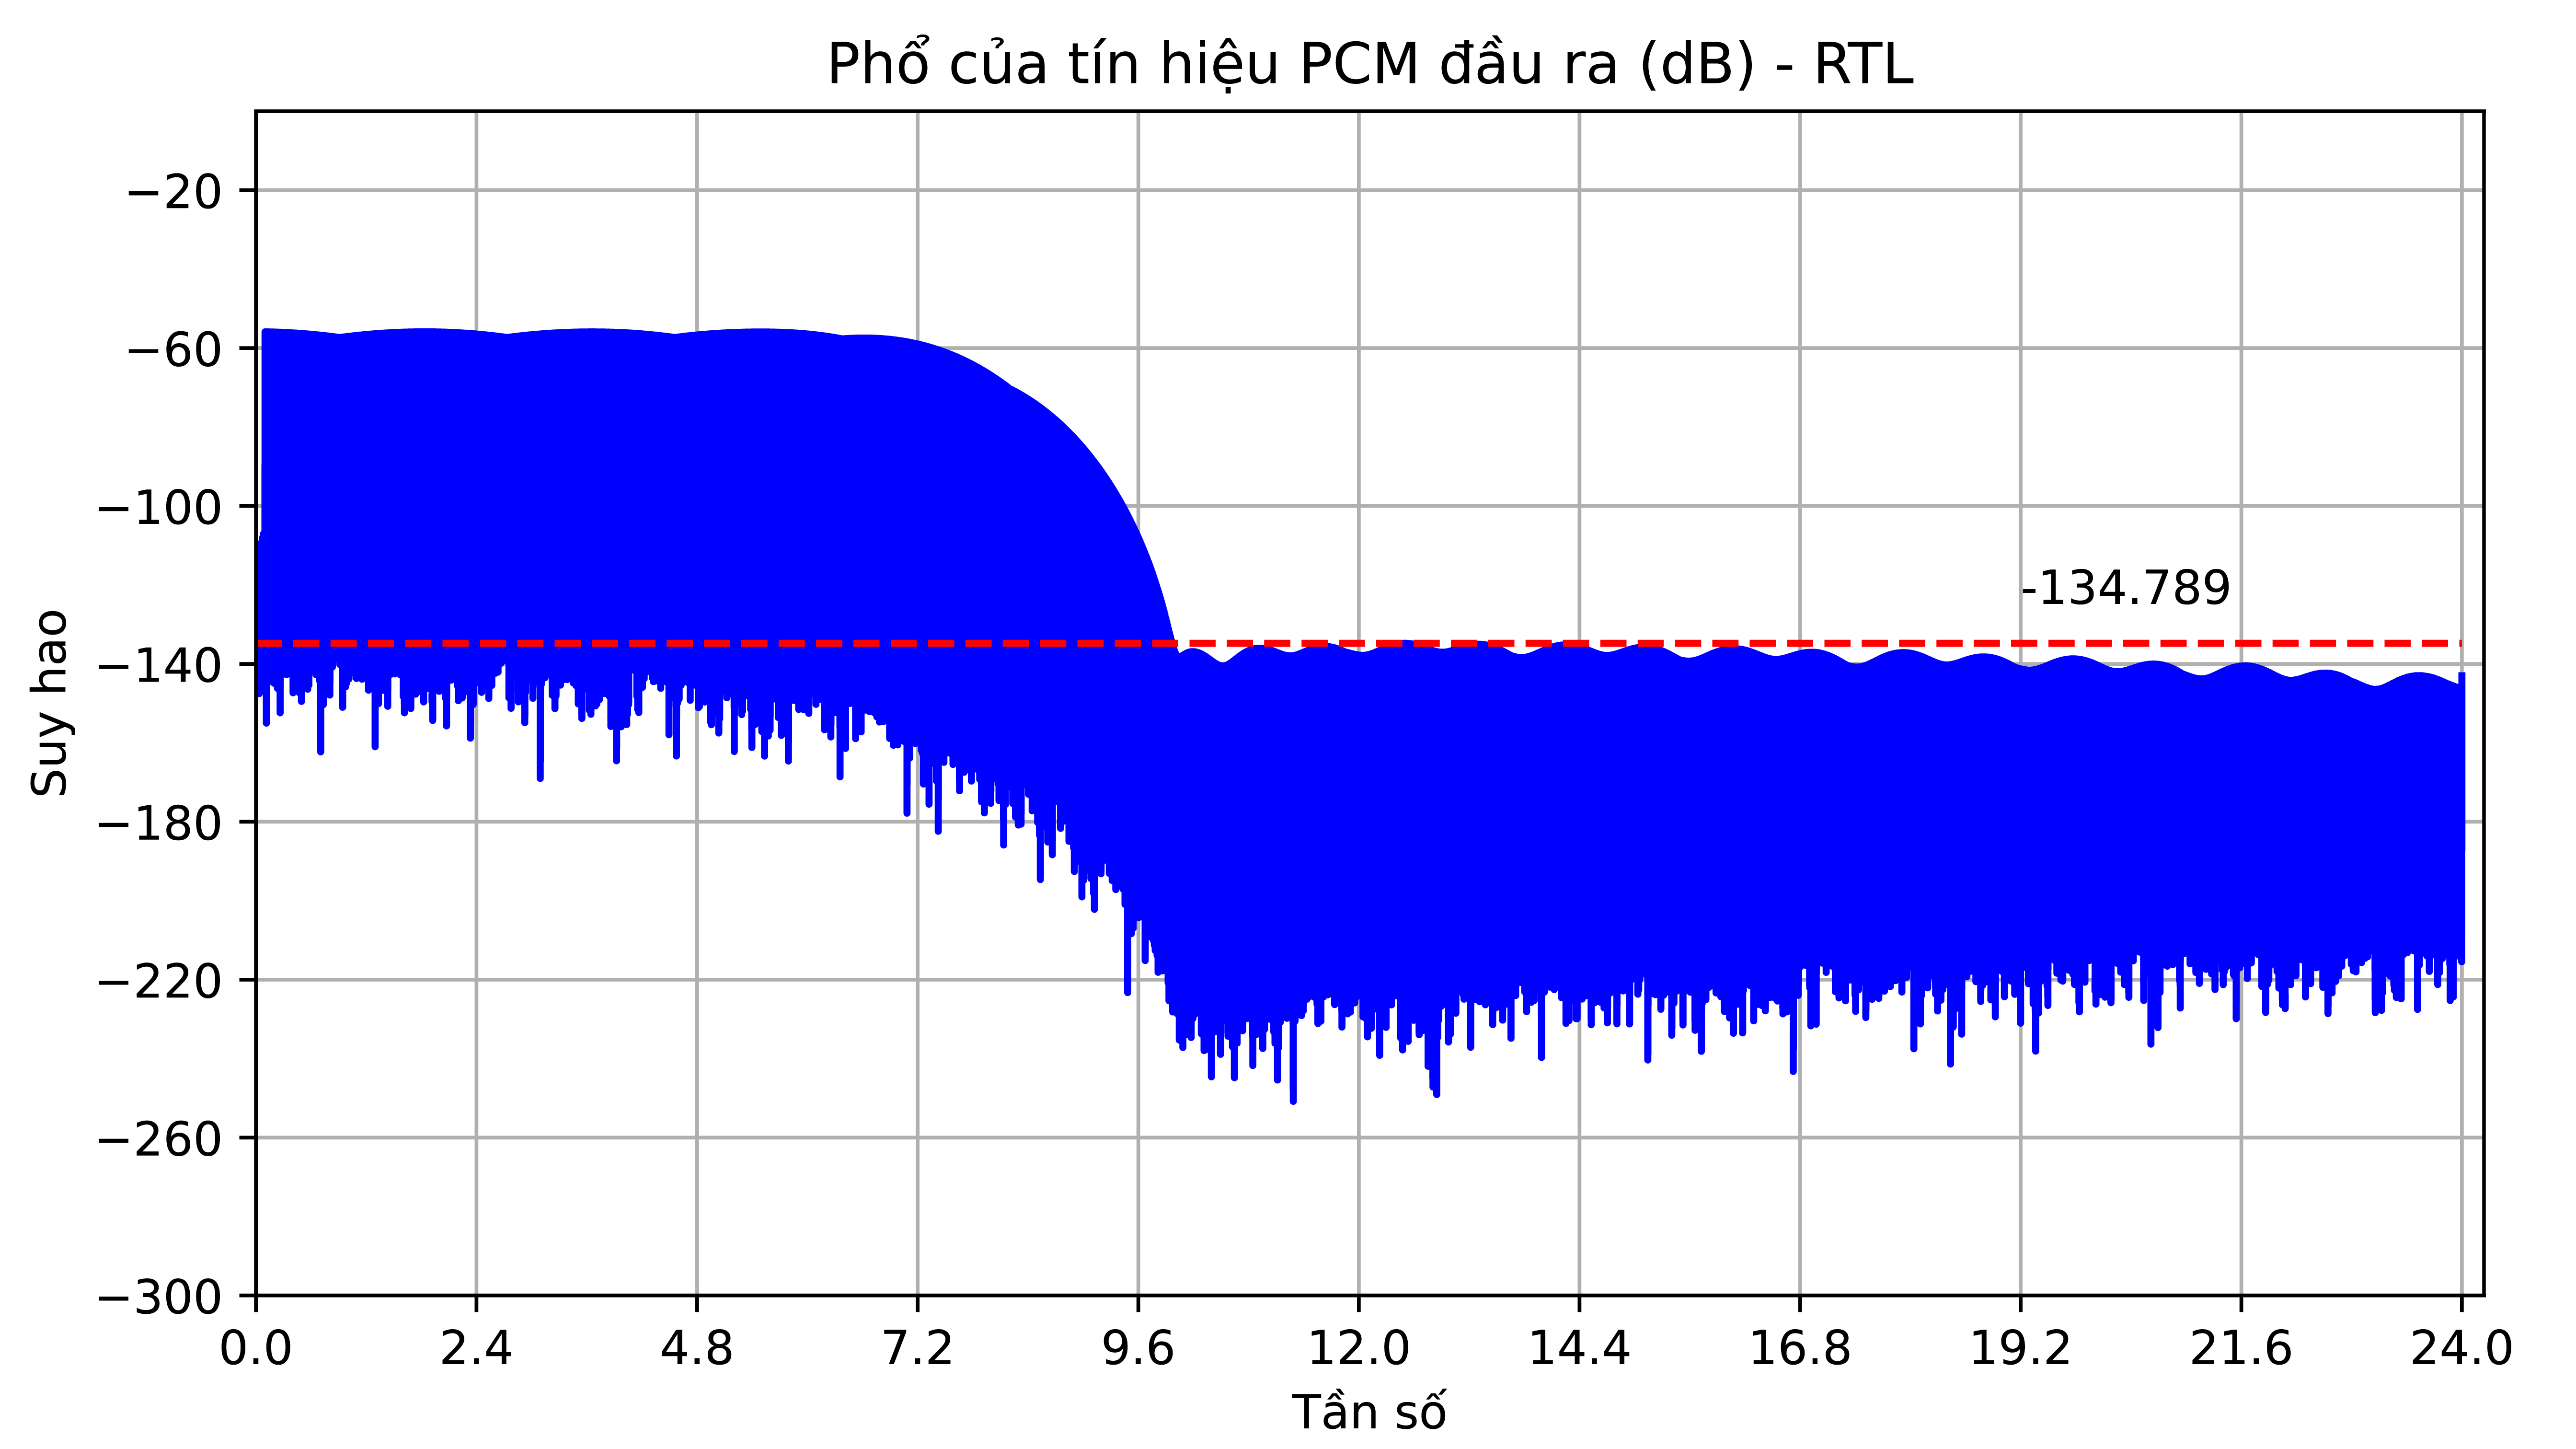
\includegraphics[width=12cm]{Images/Chuong4/tb/sim/sin_1_psd_h.png}
    \caption[Miền thời gian của tín hiệu mô phỏng bằng phần cứng]{\bfseries \fontsize{12pt}{0pt}\selectfont Miền thời gian của tín hiệu mô phỏng bằng phần cứng}
    \label{sin_1_psd_h}
\end{figure}
Nếu chúng ta lấy chuẩn của phần mềm độ suy hao dải dừng là 90.7 dB (hình \ref{d}) thì độ suy hao dải dừng của phần cứng chỉ đạt 78.768 dB, không đáp ứng được với chỉ tiêu thiết kế đặt ra là 89 dB. Những sai số đó gây ra bởi độ rộng của PCM lấy mẫu, số bit bị cắt bỏ sau mỗi tầng lọc để giảm tài nguyên và sử dụng tính toán fixed-point.

Lúc này điểm mạnh của thiết kế là linh động các bộ tham số khác nhau sẽ được phát huy. Lúc này chúng ta sẽ tăng tham số độ suy hao dải dừng lên 110 dB và đưa vào phần mềm để tính toán các "parameter" để đưa vào code RTL. Nó sẽ tự động đưa ra các tham số, các hệ số của bộ lọc để tối ưu nhất cho phần cứng. Hình \ref{filter_inc} mô tả đáp ứng xung của từng bộ lọc sau khi tăng độ suy hao dải dừng và sử dụng fixed-point (quá trình thực hiện đã được mô tả ở mục \ref{fix-fil}).

\begin{figure}[H]
    \centering
    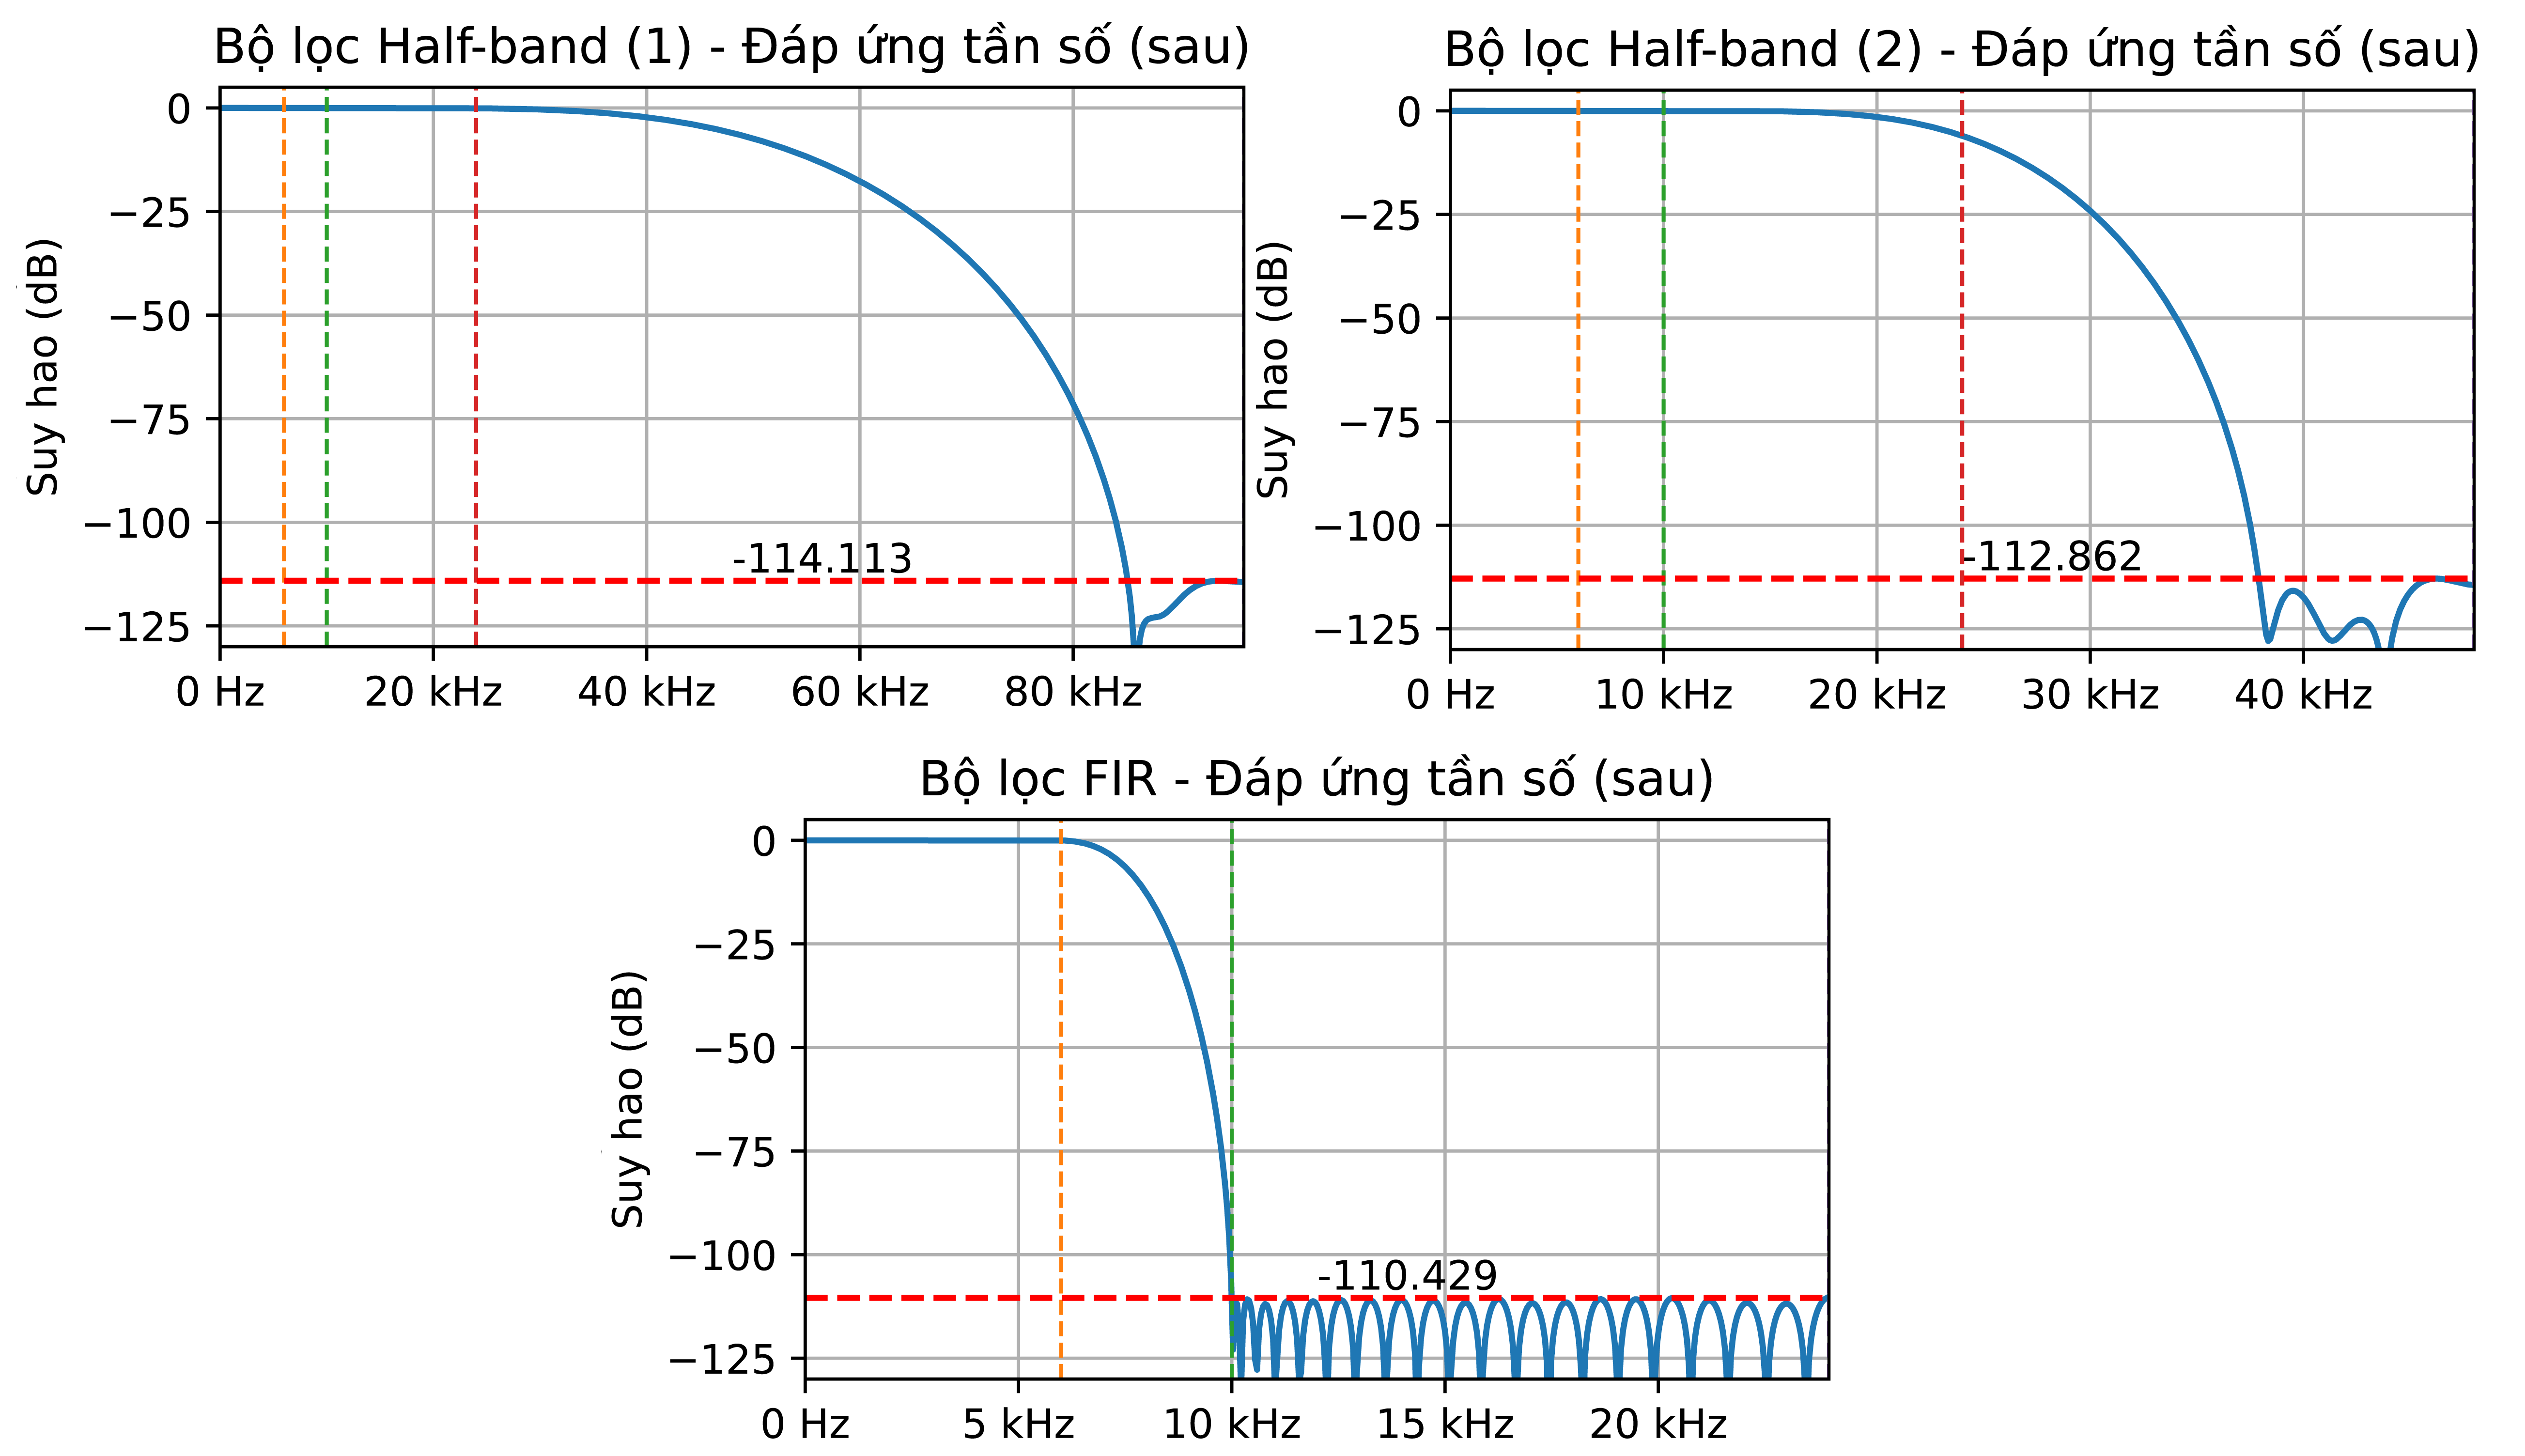
\includegraphics[width=14cm]{Images/Chuong4/tb/sim/filter_inc.png}
    \caption[Đáp ứng tần số của các bộ lọc sau  khi tăng độ suy hao dải dừng và fixed-point các hệ số]{\bfseries \fontsize{12pt}{0pt}\selectfont Đáp ứng tần số của các bộ lọc sau  khi tăng độ suy hao dải dừng và fixed-point các hệ số}
    \label{filter_inc}
\end{figure}
Lúc này số "taps" của Half Band (1), Half Band (2), FIR sẽ lần lượt là 15, 23 và 57.            
Tiến hành mô phỏng trên bộ lọc mới, chúng ta thu được tín hiệu trên miền thời gian như hình \ref{sin_2_h}.

\begin{figure}[H]
    \centering
    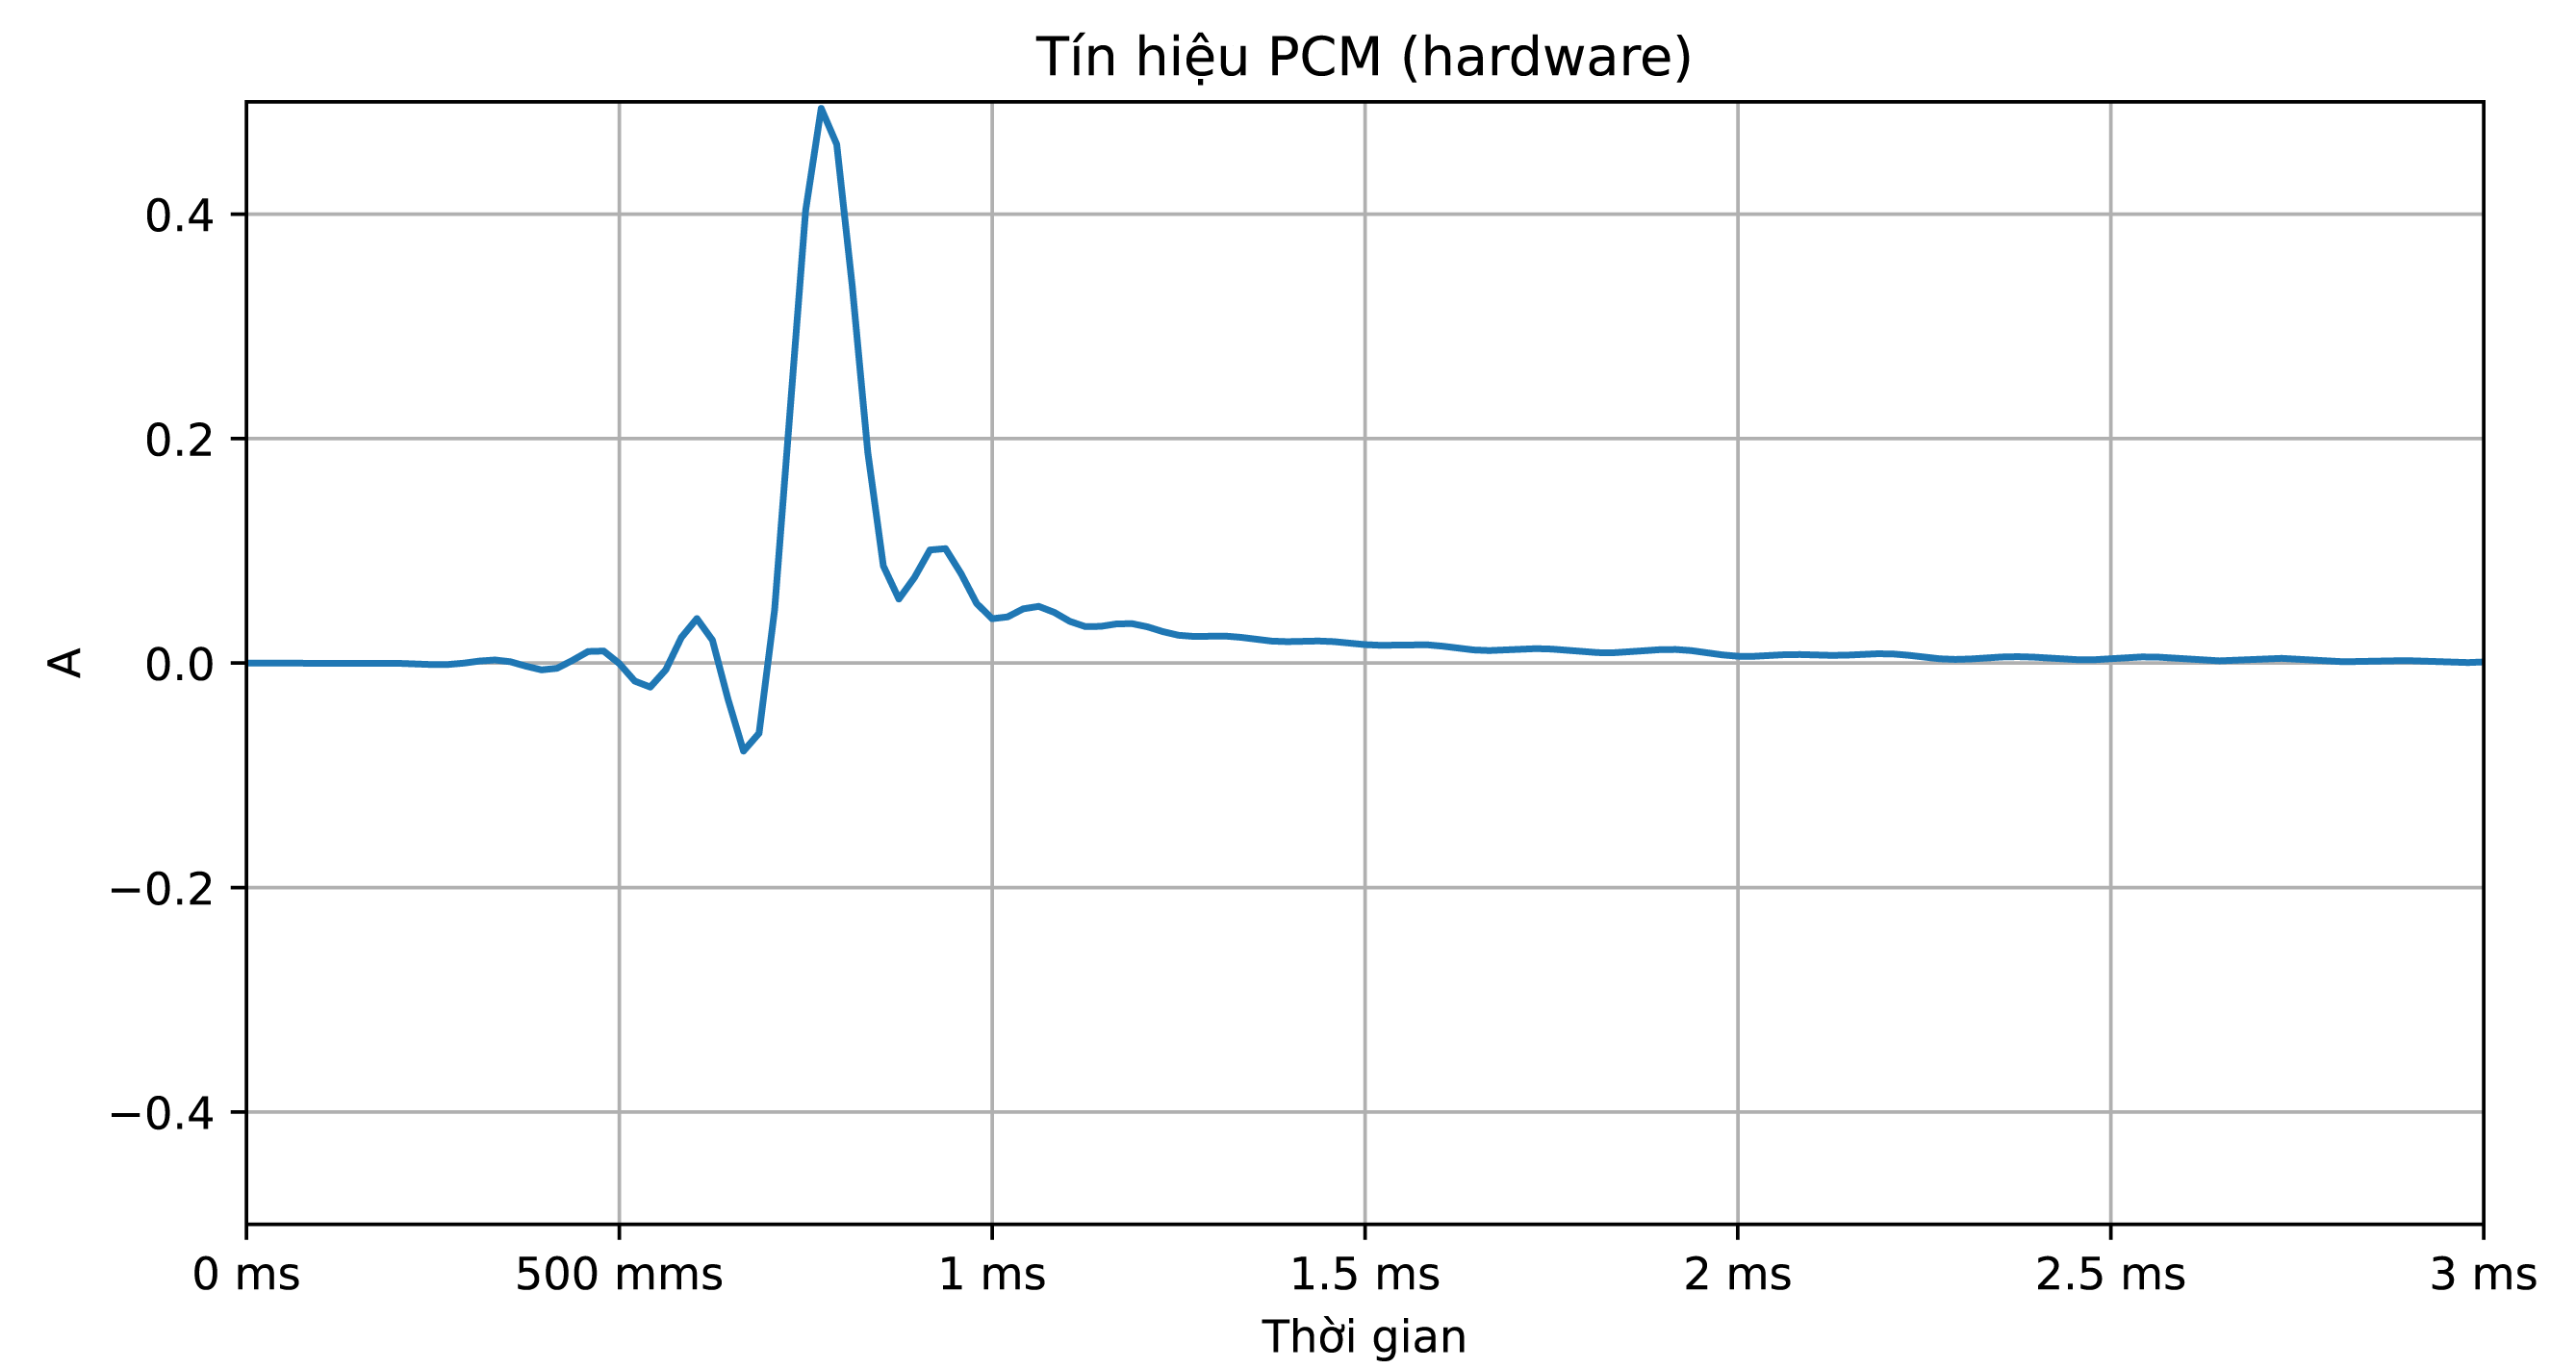
\includegraphics[width=12cm]{Images/Chuong4/tb/sim/sin_2_h.png}
    \caption[Miền thời gian của tín hiệu mô phỏng bằng phần cứng với độ suy hao mới]{\bfseries \fontsize{12pt}{0pt}\selectfont Miền thời gian của tín hiệu mô phỏng bằng phần cứng với độ suy hao mới}
    \label{sin_2_h}
\end{figure}

Hình \ref{sin_2_psd_h} mô tả phổ của tín hiệu PCM với thiết kế độ suy hao mới. Lúc này nếu lấy độ suy hao dải cao nhất ở dải dừng ở thiết kế cũ làm tham chiếu (146.721 dB) thì với bộ lọc hiện tại (147.584 dB) độ suy hao của dải dừng đã tăng lên 91.565 dB (147.584 - 146.721 + 90.7). Điều này đã hoàn toàn đáp ứng được các yêu cầu thiết kế đưa ra.

\begin{figure}[H]
    \centering
    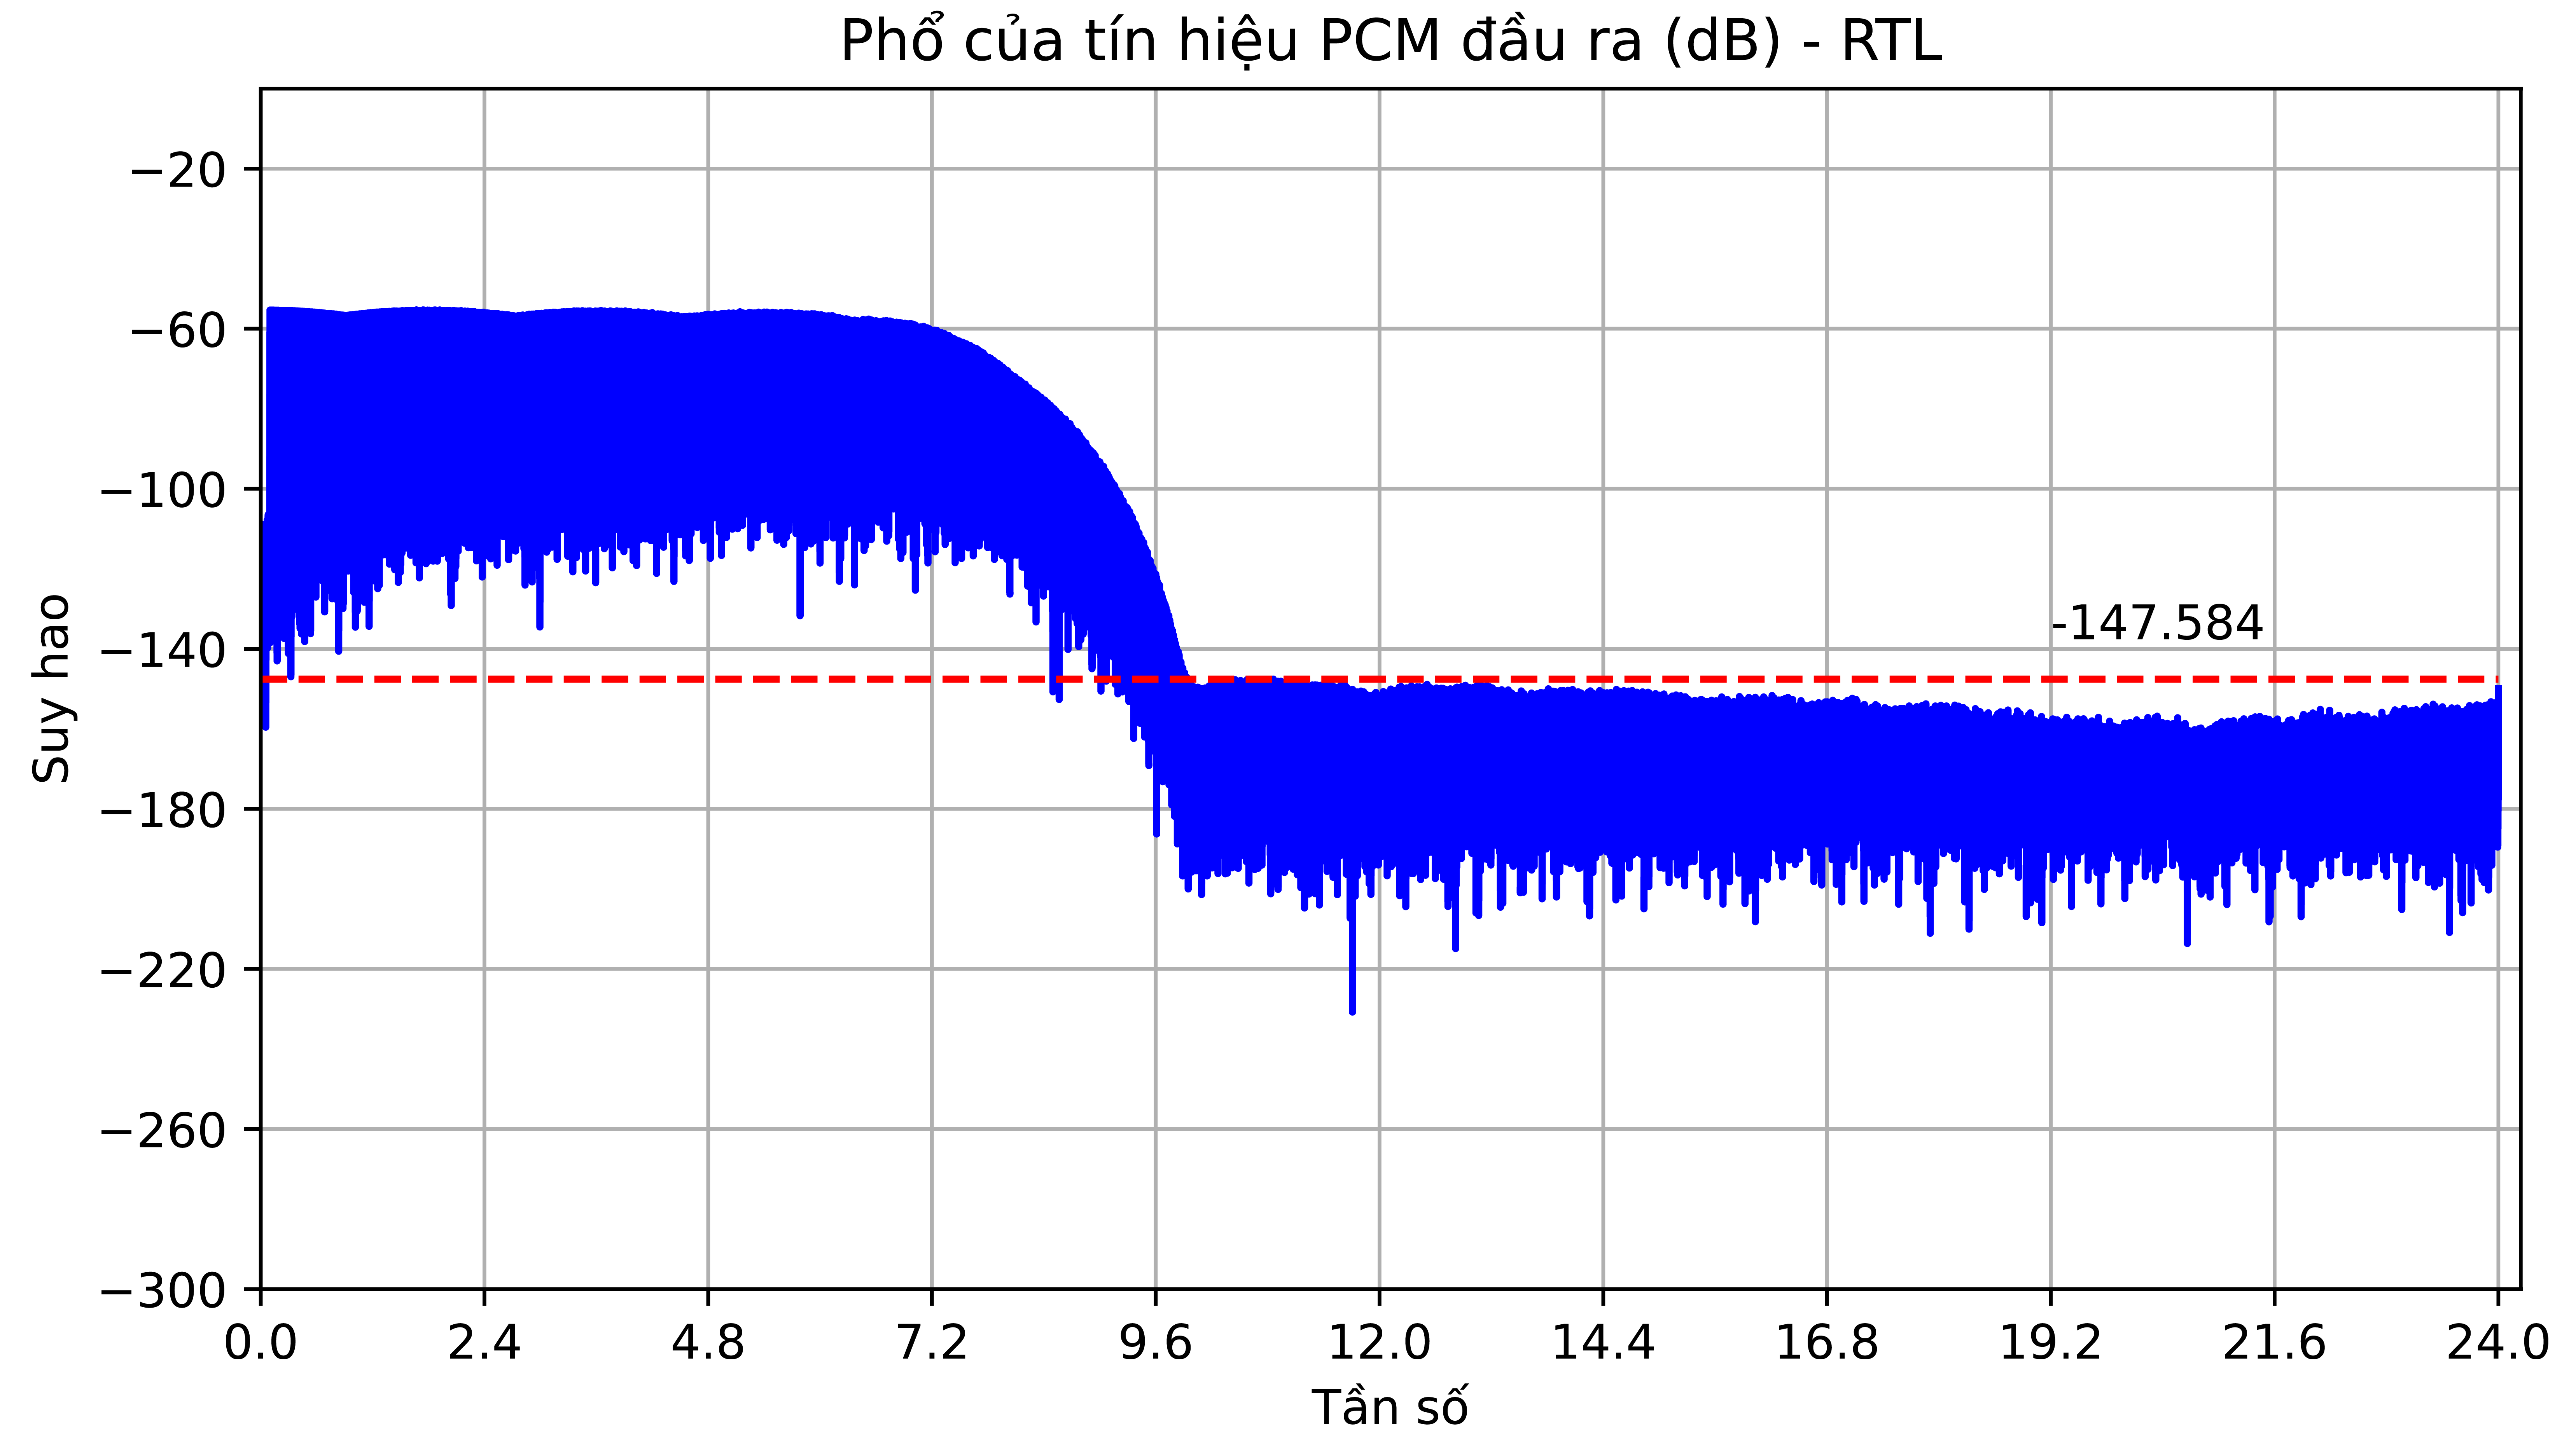
\includegraphics[width=12cm]{Images/Chuong4/tb/sim/sin_2_psd_h.png}
    \caption[Miền thời gian của tín hiệu mô phỏng bằng phần cứng với độ suy hao mới]{\bfseries \fontsize{12pt}{0pt}\selectfont Miền thời gian của tín hiệu mô phỏng bằng phần cứng với độ suy hao mới}
    \label{sin_2_psd_h}
\end{figure}

\paragraph{Tín hiệu từ tệp âm thanh có sẵn}

Có một cách khác để kiểm tra tín hiệu âm thanh thu được thực tế hơn đó là nghe bằng tai. Khi được số hóa, tín hiệu âm thanh sẽ được lưu trữ dưới dạng tệp ".wav, .mp3, \ldots" Từ các tệp này chúng ta có thể nghe lại ở mọi thiết bị và mọi thời điểm. Với tín hiệu chất lượng cao - độ phân dải là 24 bit, tần số lấy mẫu là 48 kHz nó sẽ được lưu dưới dạng tệp wav.

Vận dụng các đặc điểm đó, chúng ta sẽ tiến hành đọc dữ liệu ở tệp và sau đó điều chế Sigma-Delta để thu được tín hiệu PDM. Tín hiệu này sau đó sẽ được đưa vào testbench để chạy mô phỏng.

Tiến hành mô phỏng với tệp nhạc có cả nhạc nền và giọng hát.

\begin{figure}[H]
    \centering
    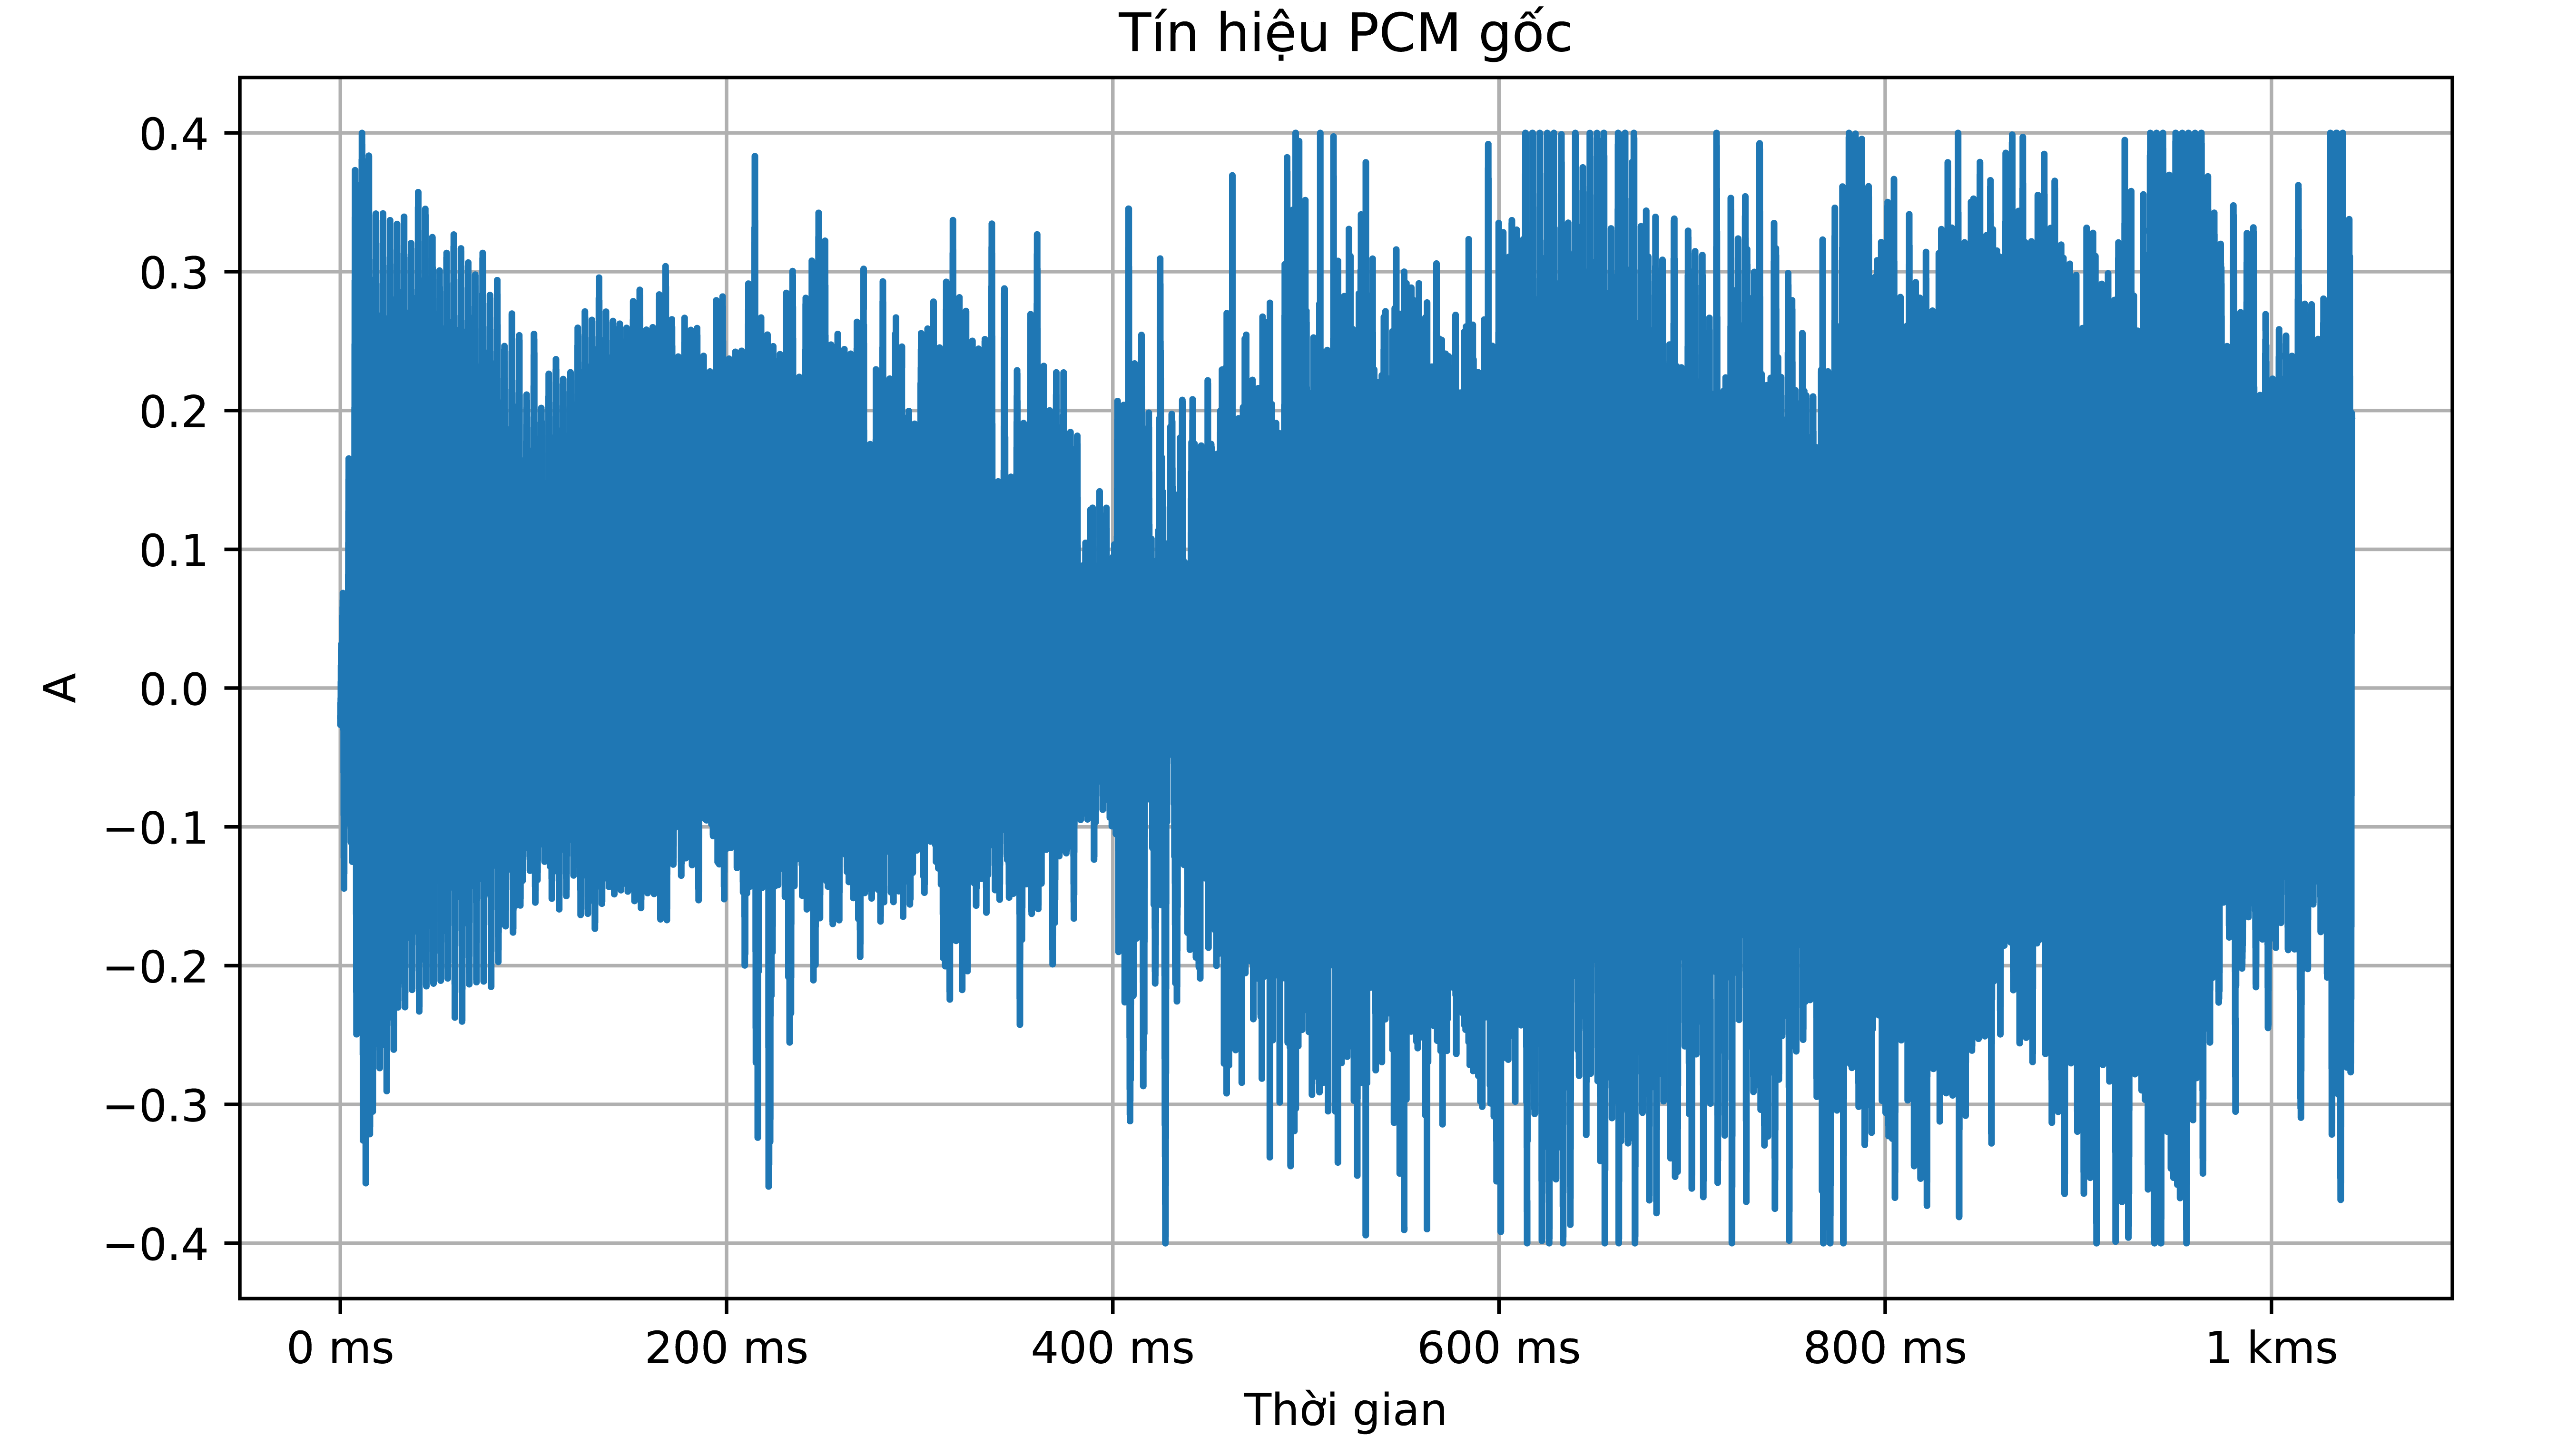
\includegraphics[width=14cm]{Images/Chuong4/tb/wav/vldd2_2.png}
    \caption[Biểu đồ miền thời gian của âm thanh gốc]{\bfseries \fontsize{12pt}{0pt}\selectfont Biểu đồ miền thời gian của âm thanh gốc}
    \label{vldd2_2}
\end{figure}

Hình \ref{vldd2_2} là biều đồ biểu thị 1 phần nhỏ tín hiệu gốc của tệp đề cập ở trên. 
\begin{figure}[H]
    \centering
    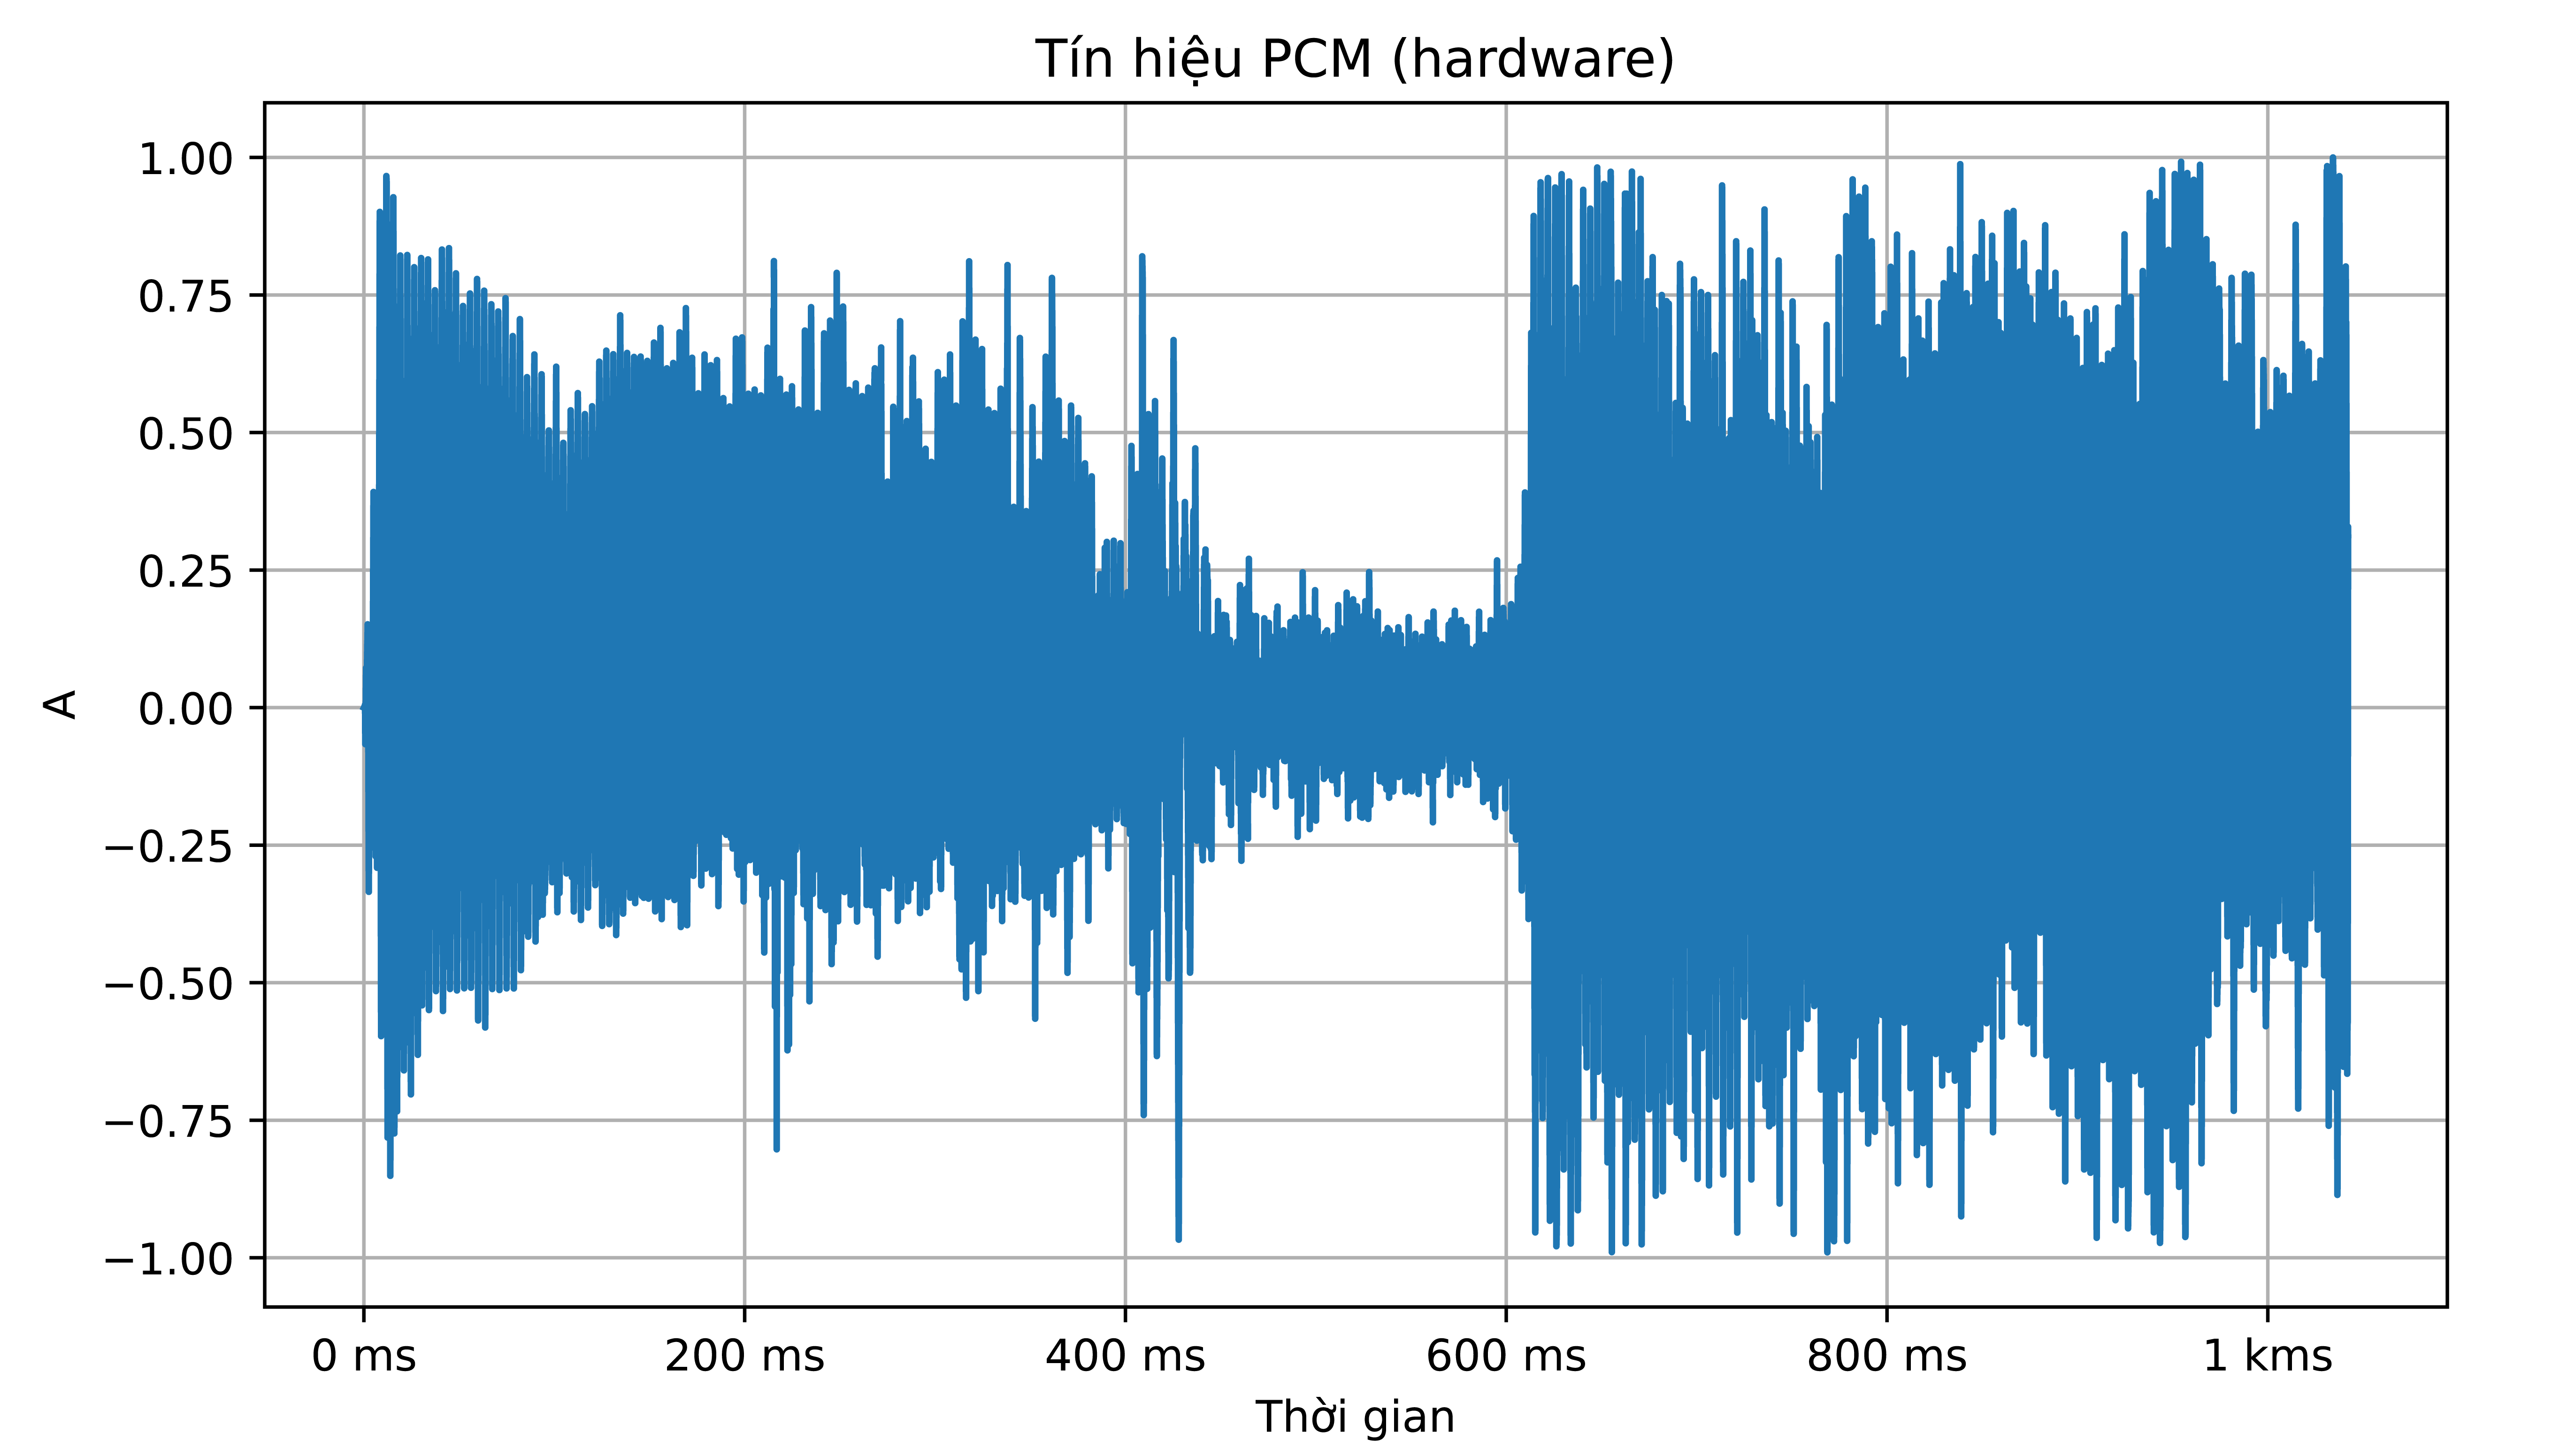
\includegraphics[width=14cm]{Images/Chuong4/tb/wav/vldd2_0.png}
    \caption[Biểu đồ miền thời gian của âm thanh sau khi đi qua bộ chuyển đổi]{\bfseries \fontsize{12pt}{0pt}\selectfont  Biểu đồ miền thời gian của âm thanh sau khi đi qua bộ chuyển đổi }
    \label{vldd2_0}
\end{figure}

\begin{figure}[H]
    \centering
    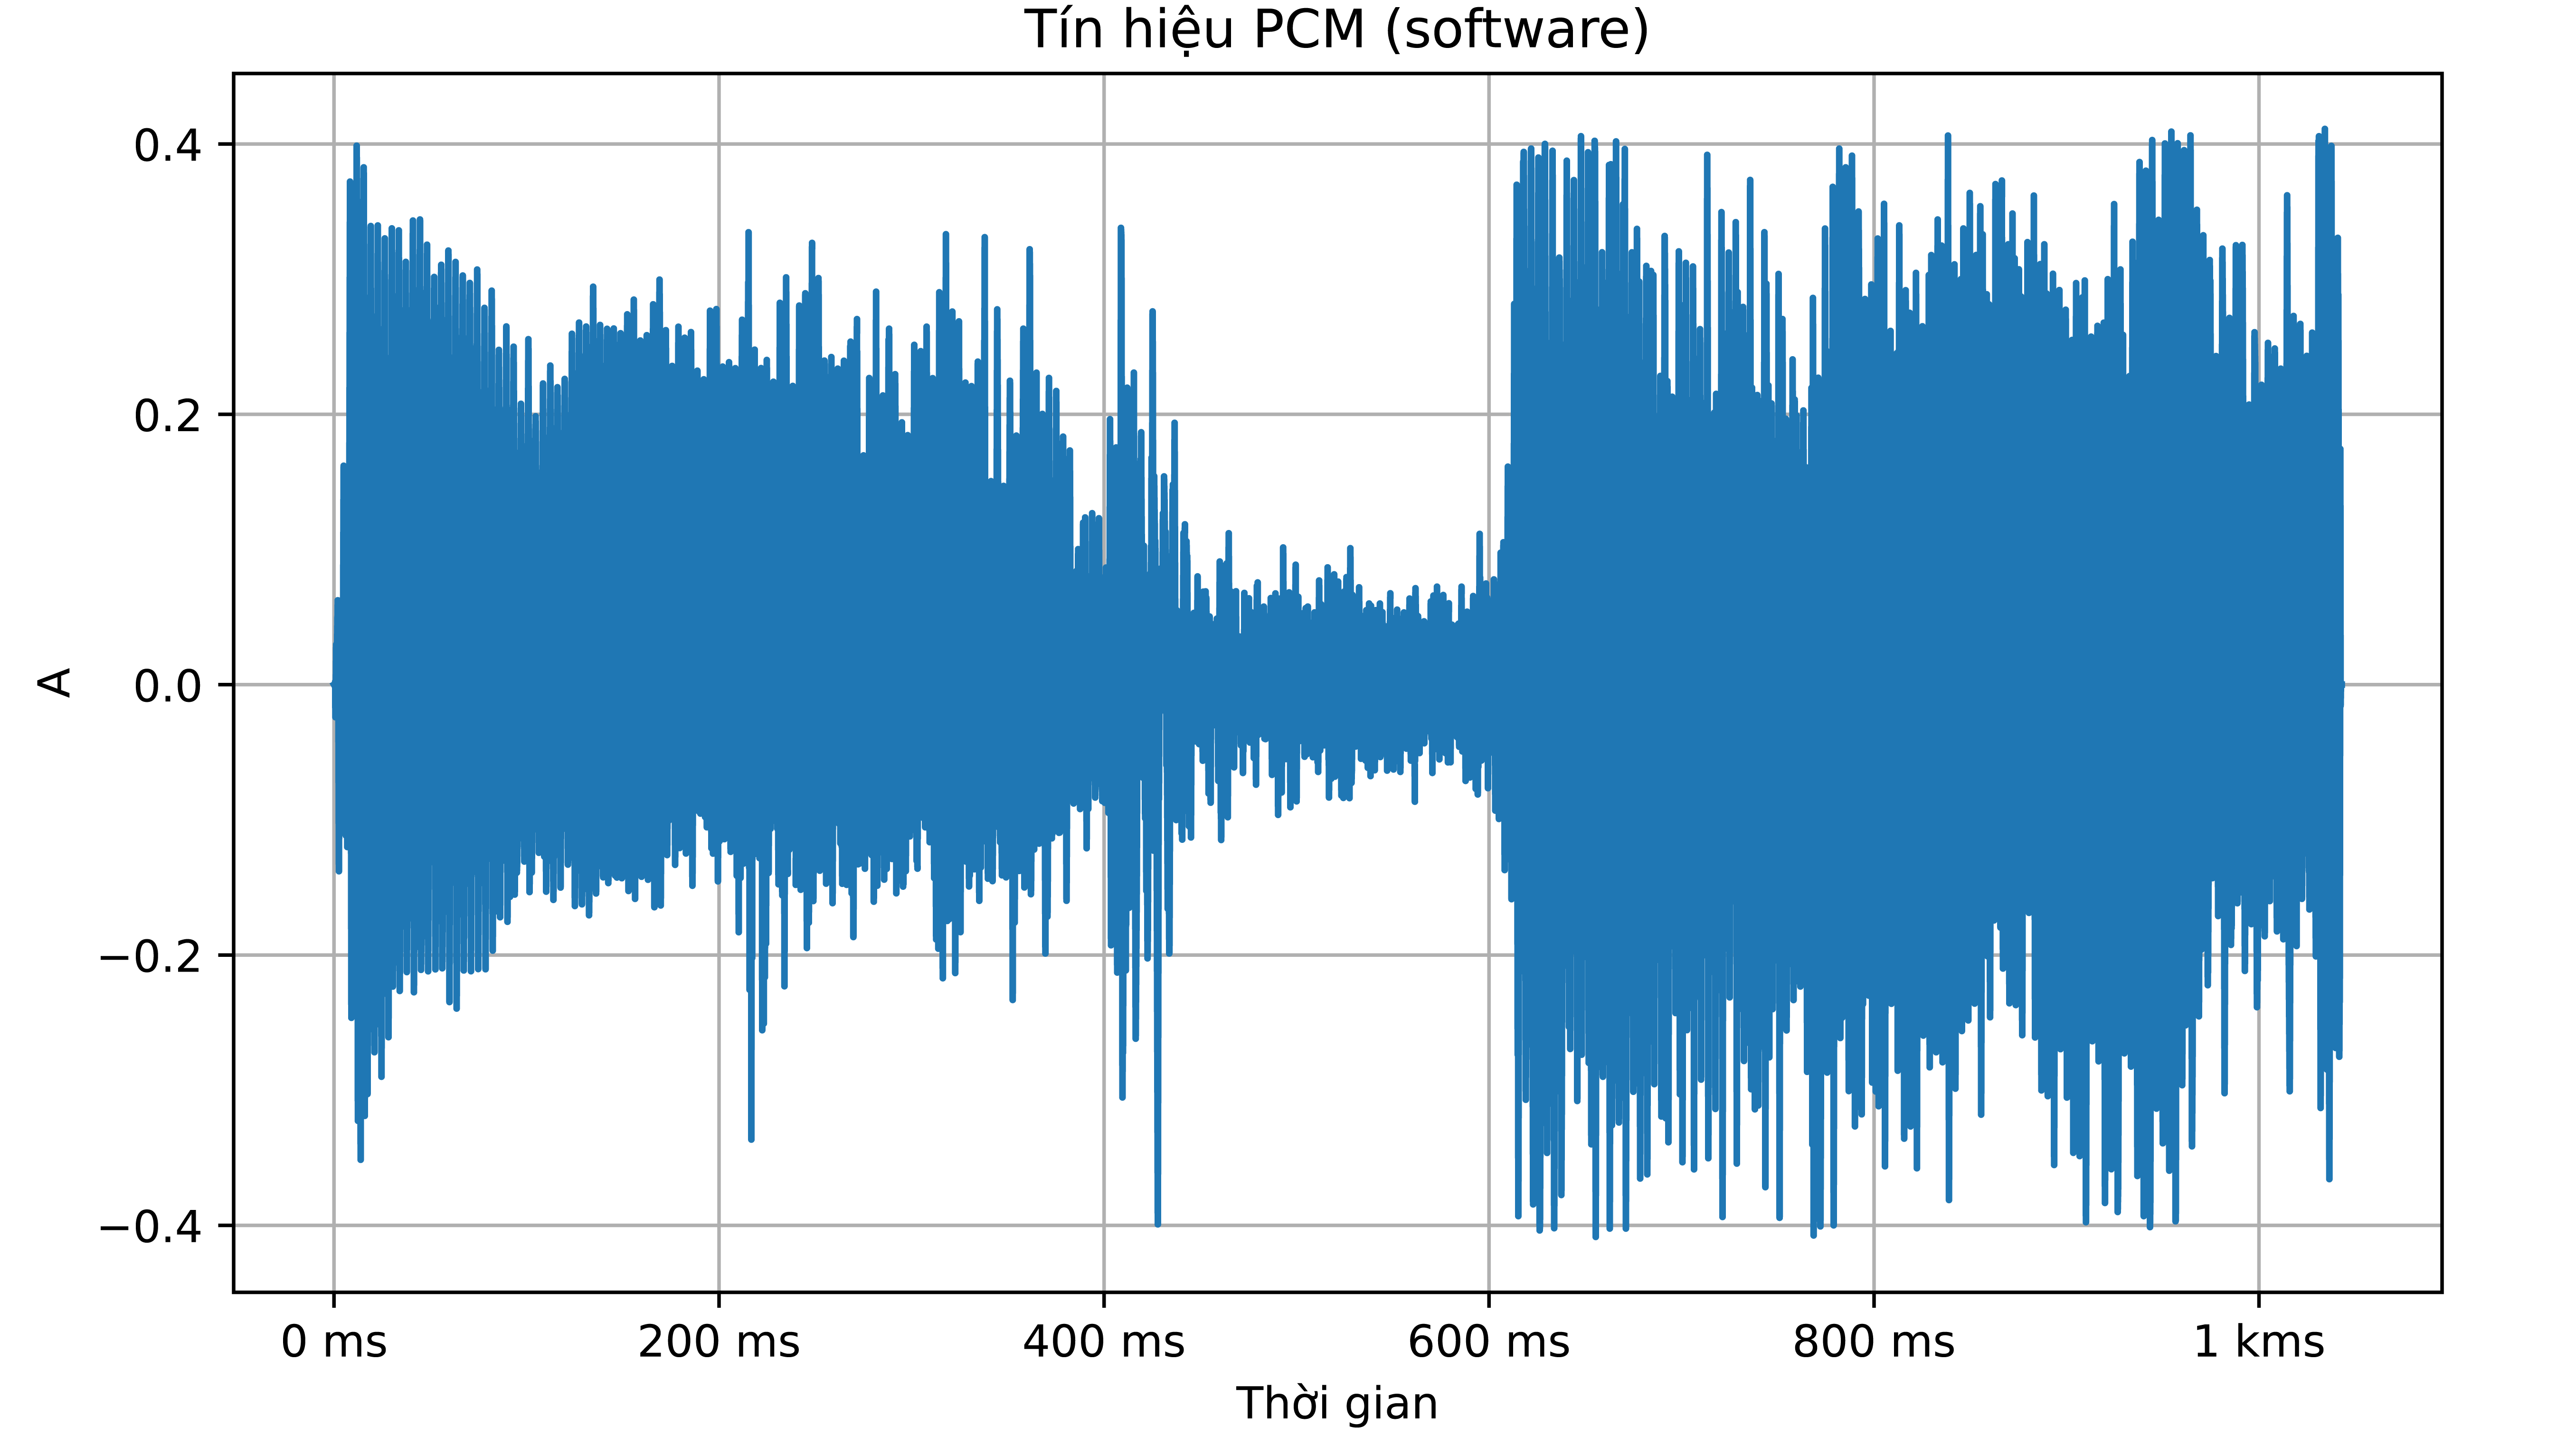
\includegraphics[width=14cm]{Images/Chuong4/tb/wav/vldd2_1.png}
    \caption[Biểu đồ miền thời gian của âm thanh sau sau khi chuyển đổi bằng phần mềm]{\bfseries \fontsize{12pt}{0pt}\selectfont  Biểu đồ miền thời gian của âm thanh sau sau khi chuyển đổi bằng phần mềm}
    \label{vldd2_1}
\end{figure}
Sau khi đi qua bộ chuyển đổi bằng phần cứng (hình \ref{vldd2_0}) và bộ chuyển đổi sử dụng tính toán bằng phần mềm (hình \ref{vldd2_1}), ta thấy được sự khác biệt giữa các biểu đồ trước và sau mô phỏng. Tín hiệu gốc đã mất đi một phần tín hiệu nào đó khiến nó bị biến dạng. Tuy nhiên biểu đồ giữa mô phỏng bằng phần cứng và phần mềm lại tương tự nhau. Để hiểu rõ chi tiết hơn, chúng ta nên xem các tín hiệu trên biểu diễn trên miền tần số.

\begin{figure}[H]
    \centering
    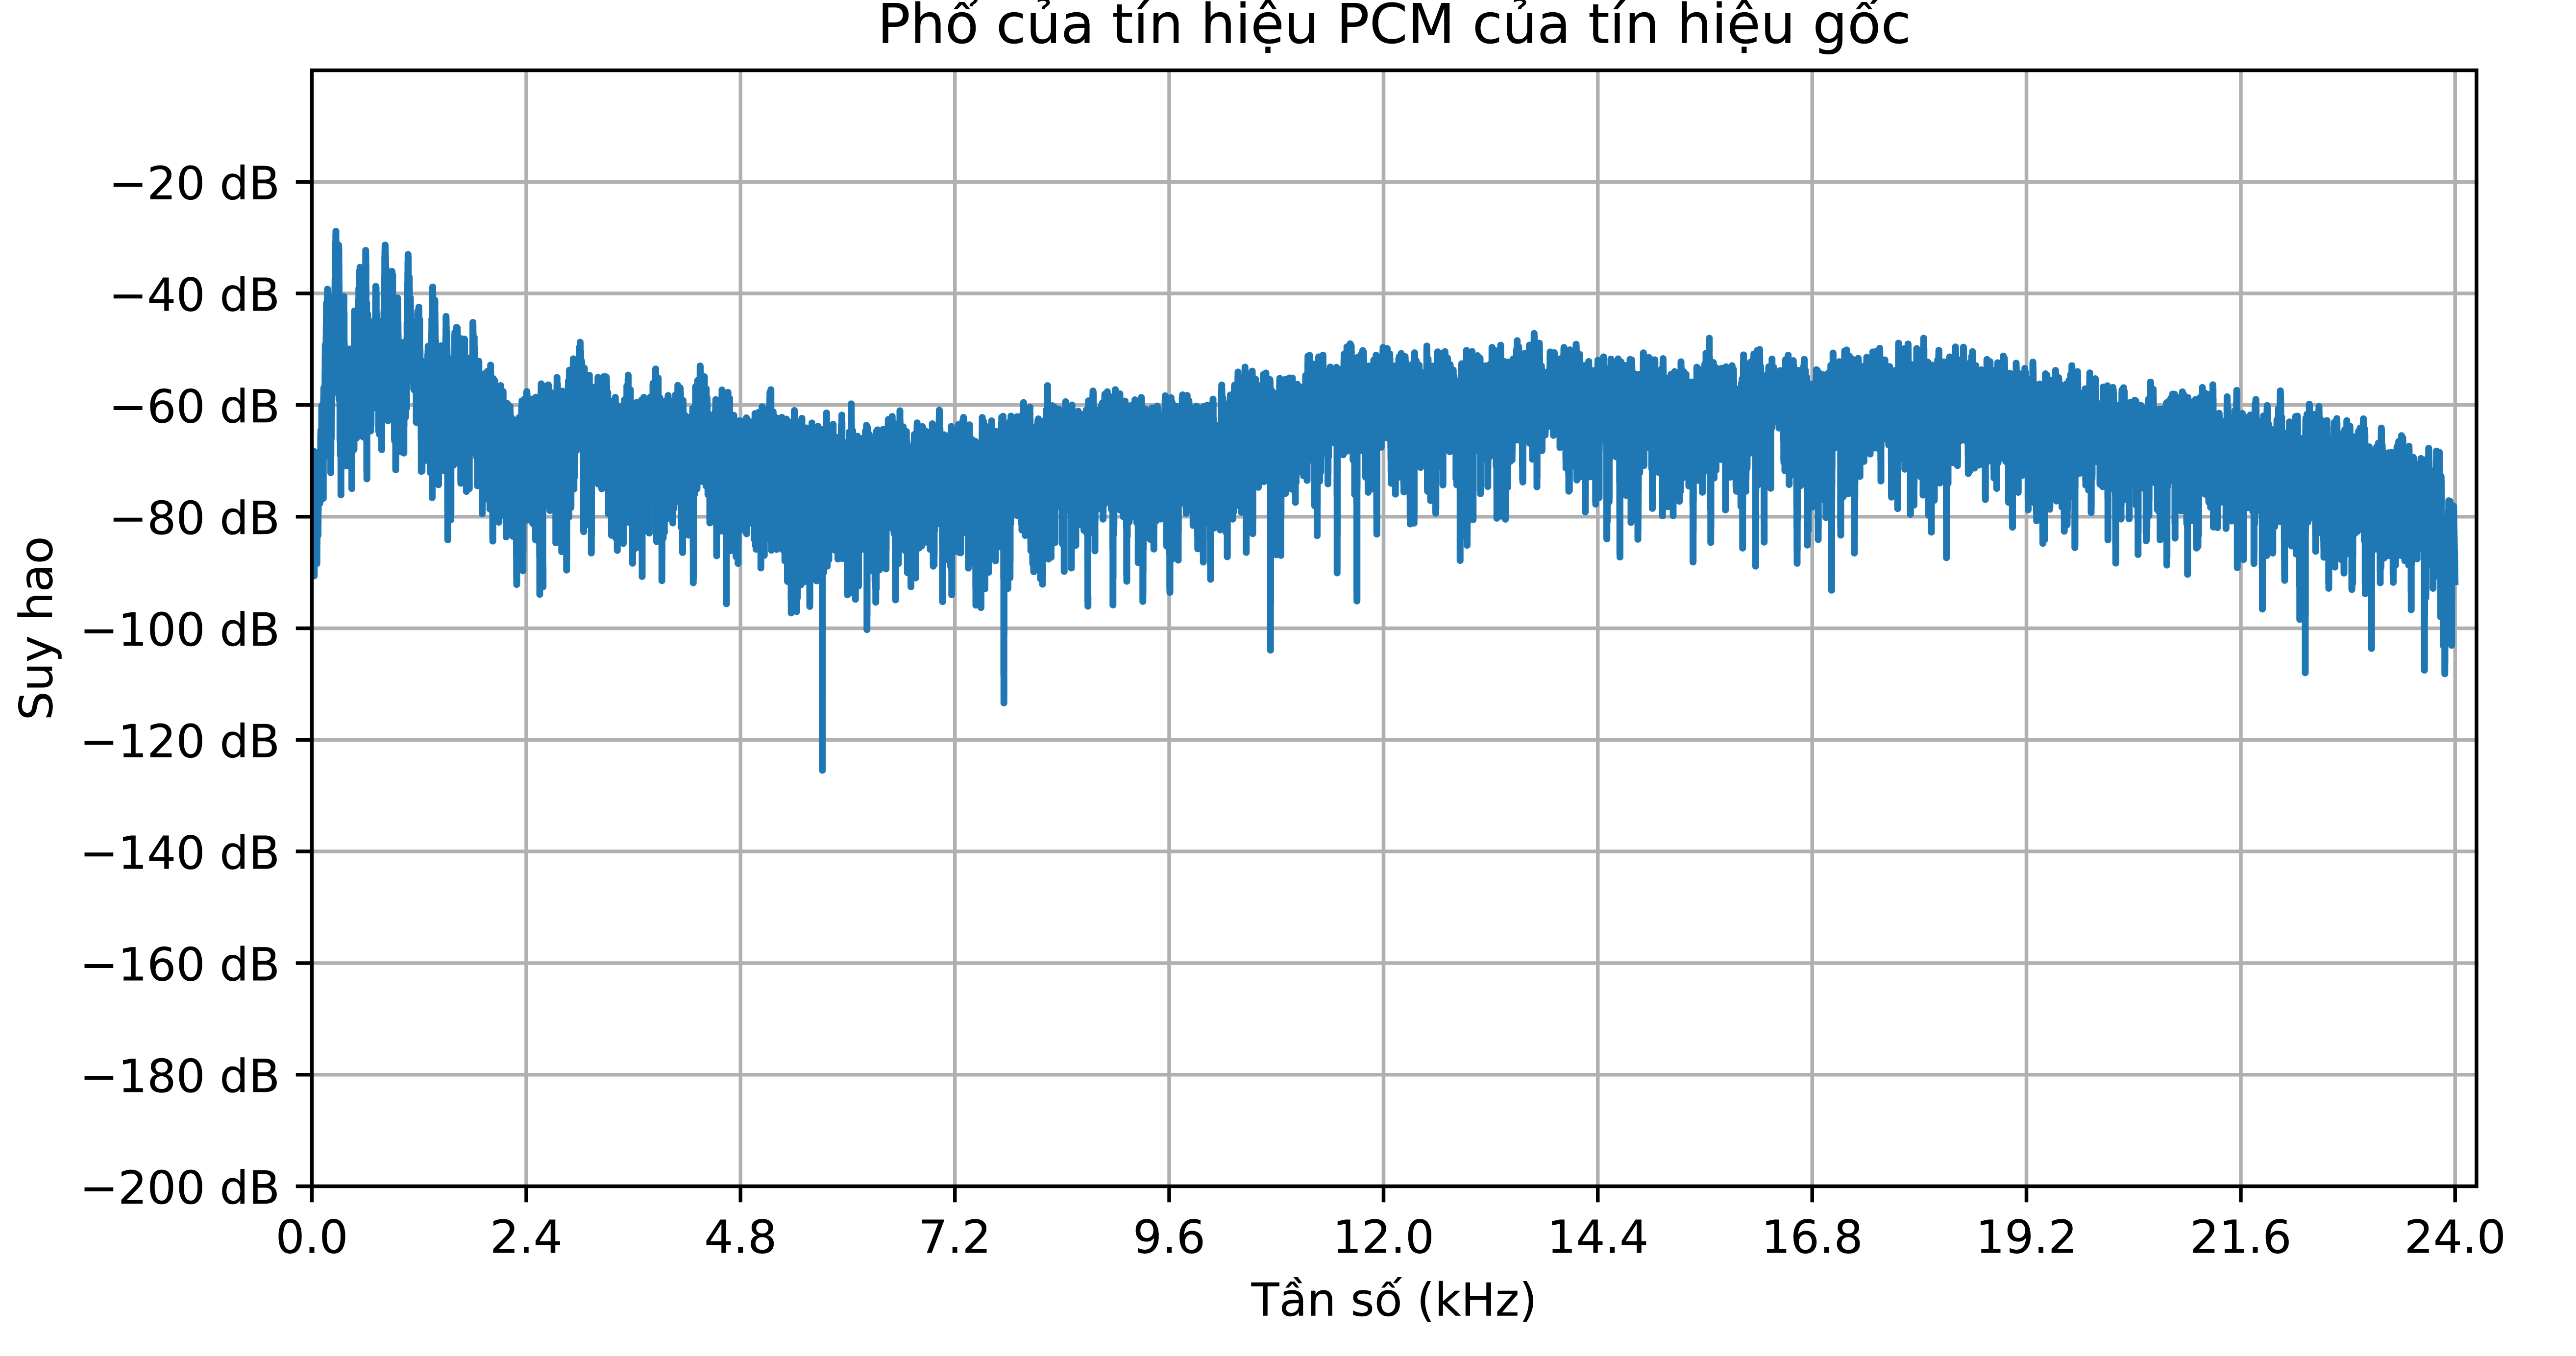
\includegraphics[width=14cm]{Images/Chuong4/tb/wav/vldd2_psd_2.png}
    \caption[Biểu đồ phổ của tín hiệu âm thanh gốc]{\bfseries \fontsize{12pt}{0pt}\selectfont Biểu đồ phổ của tín hiệu âm thanh gốc}
    \label{vldd2_psd_2}
\end{figure}



Hình \ref{vldd2_psd_2} mô tả mật độ phổ công suất của tín hiệu gốc. Chúng ta có thể thấy tín hiệu sẽ có đủ dải từ 0 - 24 kHz. Sau khi đưa qua mô phỏng tín hiệu đã bị lọc bỏ hết thành phần từ 6 - 24 kHz, điều này khiến ở miền thời gian tín hiệu sau khi chuyển đổi bị biến dạng. Hình \ref{vldd2_psd_0} và \ref{vldd2_psd_1} lần lượt là phổ của tín hiệu âm thanh sau khi đi qua mô phỏng phần cứng và phần mềm. Chúng ta có thể thấy ở dải thông, các thành phần tín hiệu ở dải tần số ở hai biểu đồ có độ suy hao giống nhau. Nó chỉ khác biệt là khi chuyển xuống dải dừng, độ suy hao của phần cứng sẽ chênh lệch với phần mềm khoảng 10 dB. Như đã đề cập ở phần trước thì độ chênh lệnh này không ảnh hưởng so với yêu cầu thiết kế là 89 dB.

Khi nghe lại 2 tệp âm thanh trước và sau khi chuyển đổi bằng phần cứng, chúng ta có nhận xét sau đây: âm thanh sau khi chuyển đổi mất đi sự chi tiết, tươi sáng và sắc bén.

Vì bộ chuyển đổi sẽ loại bỏ đi các thành phần ở tần số 6 - 24 kHz, thật trùng hợp vì đây cũng là dải tần số \textbf{Treble} (6 kHz - 20 kHz) của âm thanh. Mà dải này đảm nhận vai trò tăng độ chi tiết cho âm thanh, do đó tín hiệu nghe được bị mất cảm xúc cũng là điều hoàn toàn đúng.

\begin{figure}[H]
    \centering
    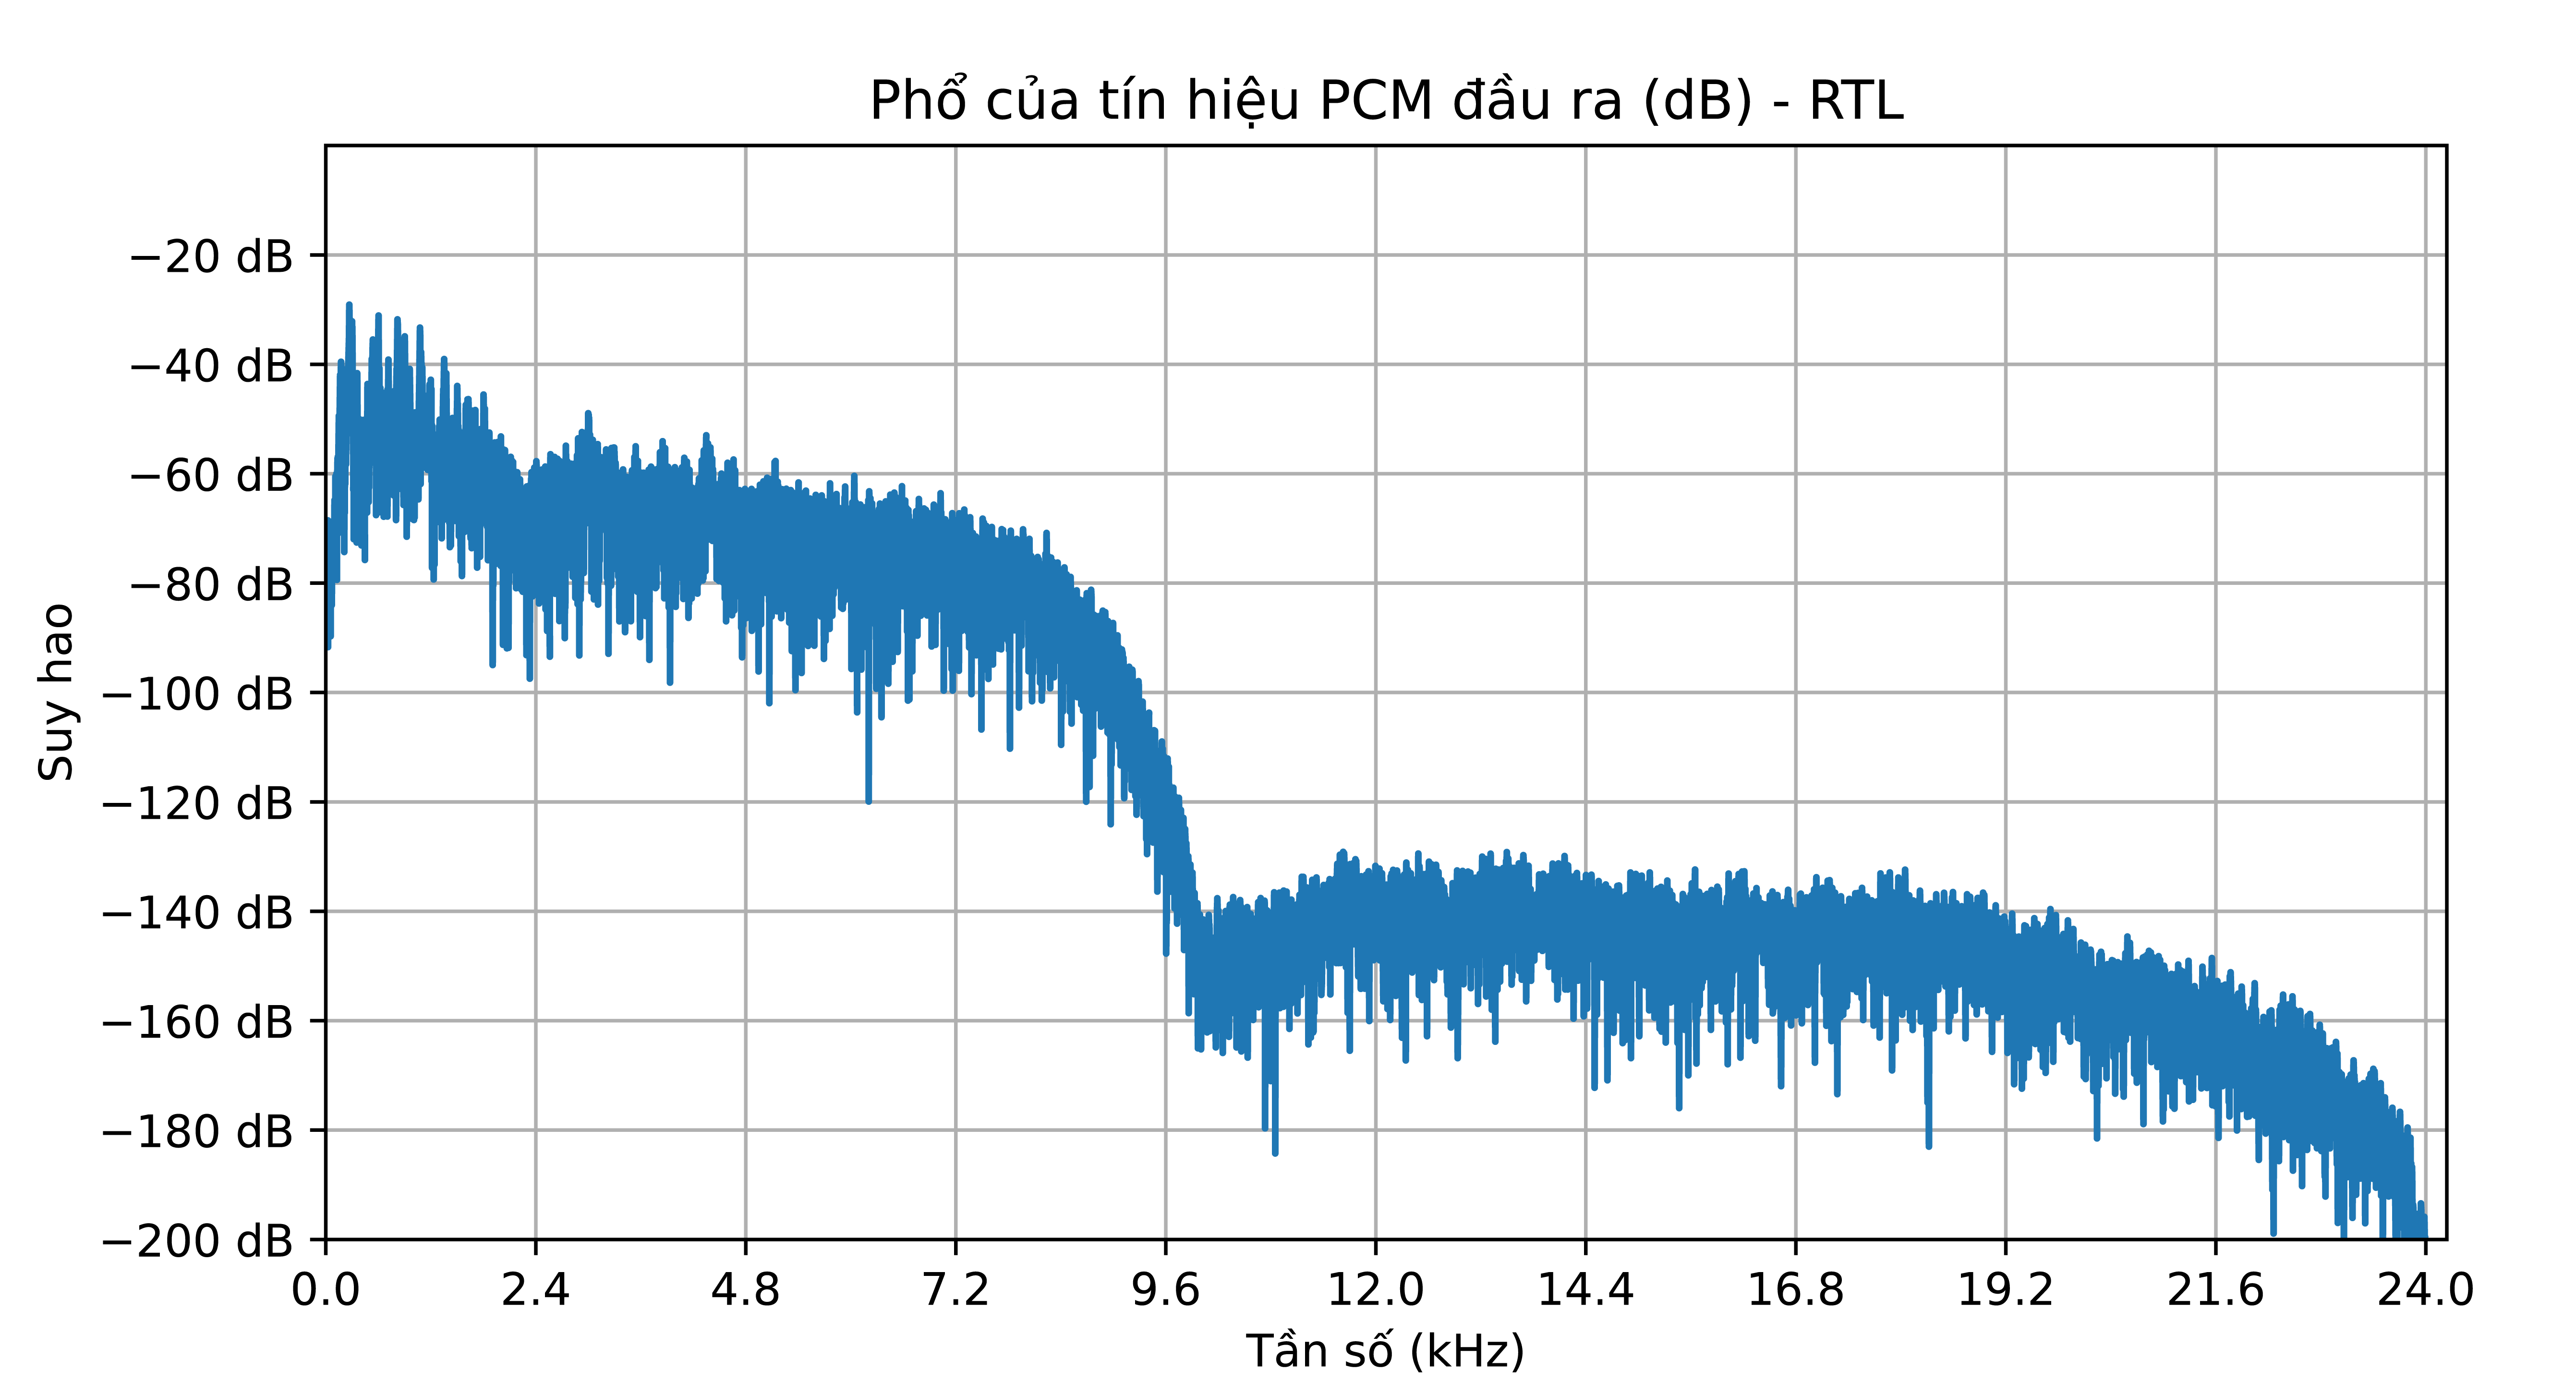
\includegraphics[width=13cm]{Images/Chuong4/tb/wav/vldd2_psd_0.png}
    \caption[Biểu đồ phổ của âm thanh sau khi chuyển đổi bằng phần cứng]{\bfseries \fontsize{12pt}{0pt}\selectfont  Biểu đồ phổ của âm thanh sau khi chuyển đổi bằng phần cứng}
    \label{vldd2_psd_0}
\end{figure}

\begin{figure}[H]
    \centering
    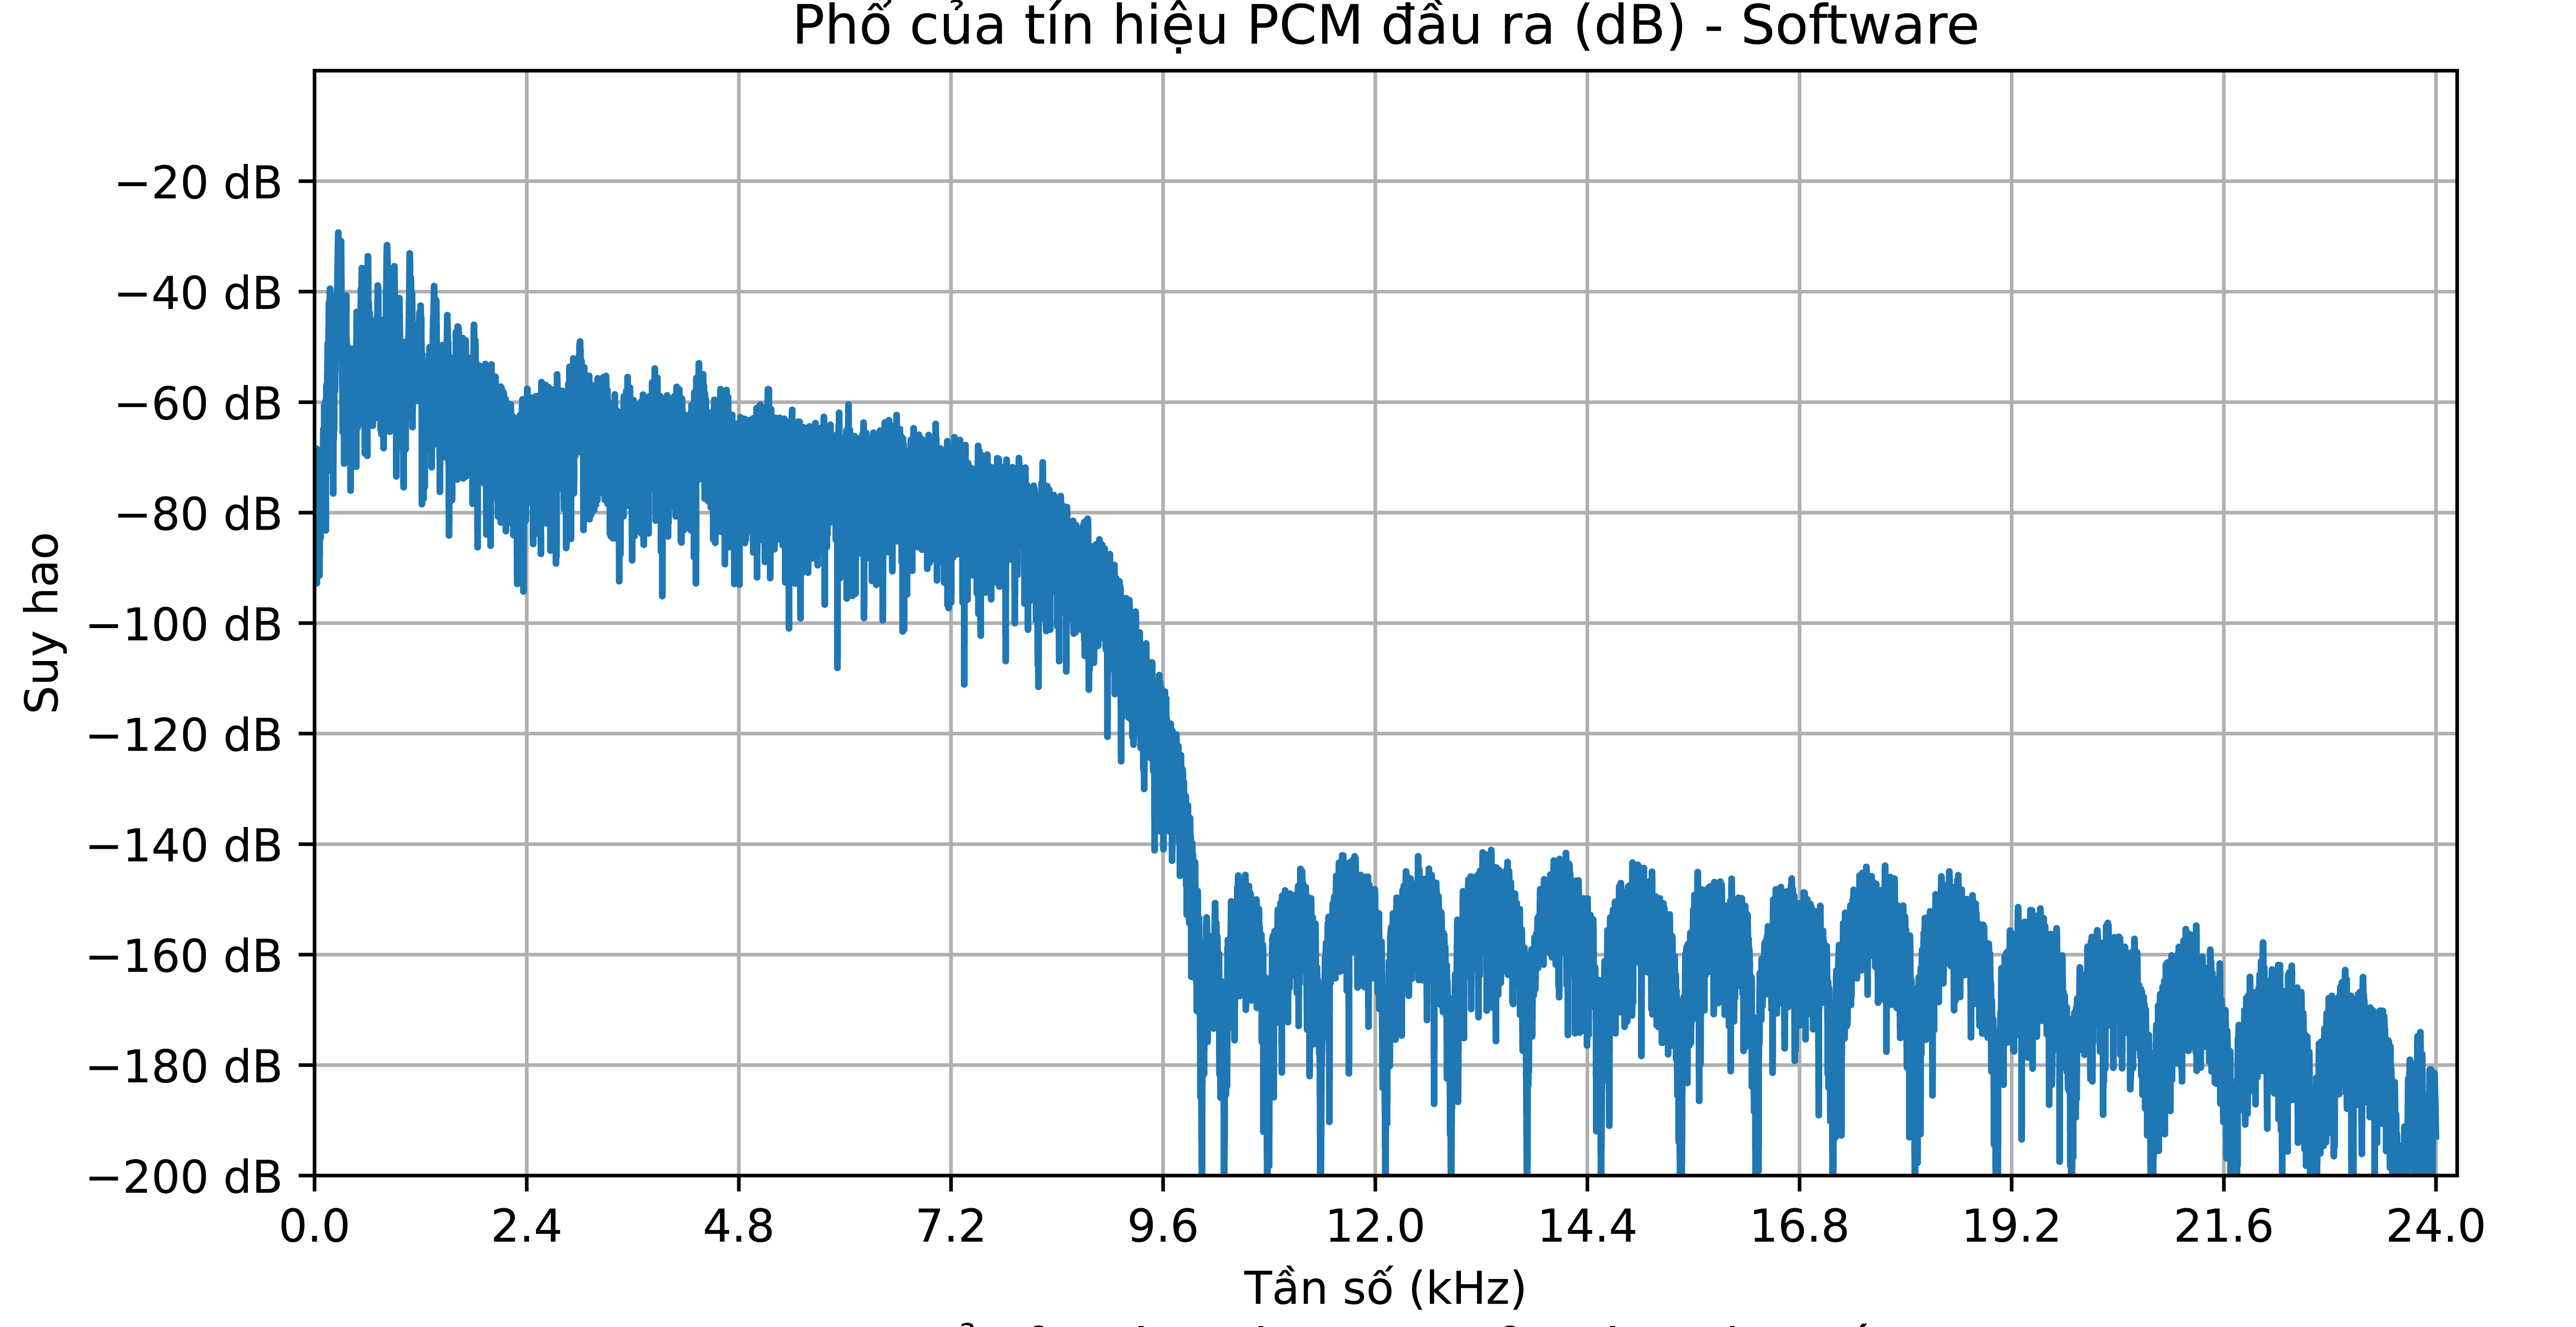
\includegraphics[width=13cm]{Images/Chuong4/tb/wav/vldd2_psd_1.png}
    \caption[Biểu đồ phổ của âm thanh sau sau khi chuyển đổi bằng phần mềm]{\bfseries \fontsize{12pt}{0pt}\selectfont  Biểu đồ phổ của âm thanh sau sau khi chuyển đổi bằng phần mềm}
    \label{vldd2_psd_1}
\end{figure}

Tiến hành mô phỏng với tệp nhạc chỉ có giọng người.

Quan sát hình \ref{vocal_psd}, tín hiệu đầu vào gốc chỉ ổn định đến tần số 10 kHz, đồng nghĩa với việc giọng nói không thu đủ dài tần (giống với dải thu của microphone đã giới thiệu ở trên). Tín hiệu sau qua bộ chuyển đổi có phổ đã đáp ứng được yêu cầu thiết kế đã đặt ra từ trước.

\begin{figure}[H]
    \centering
    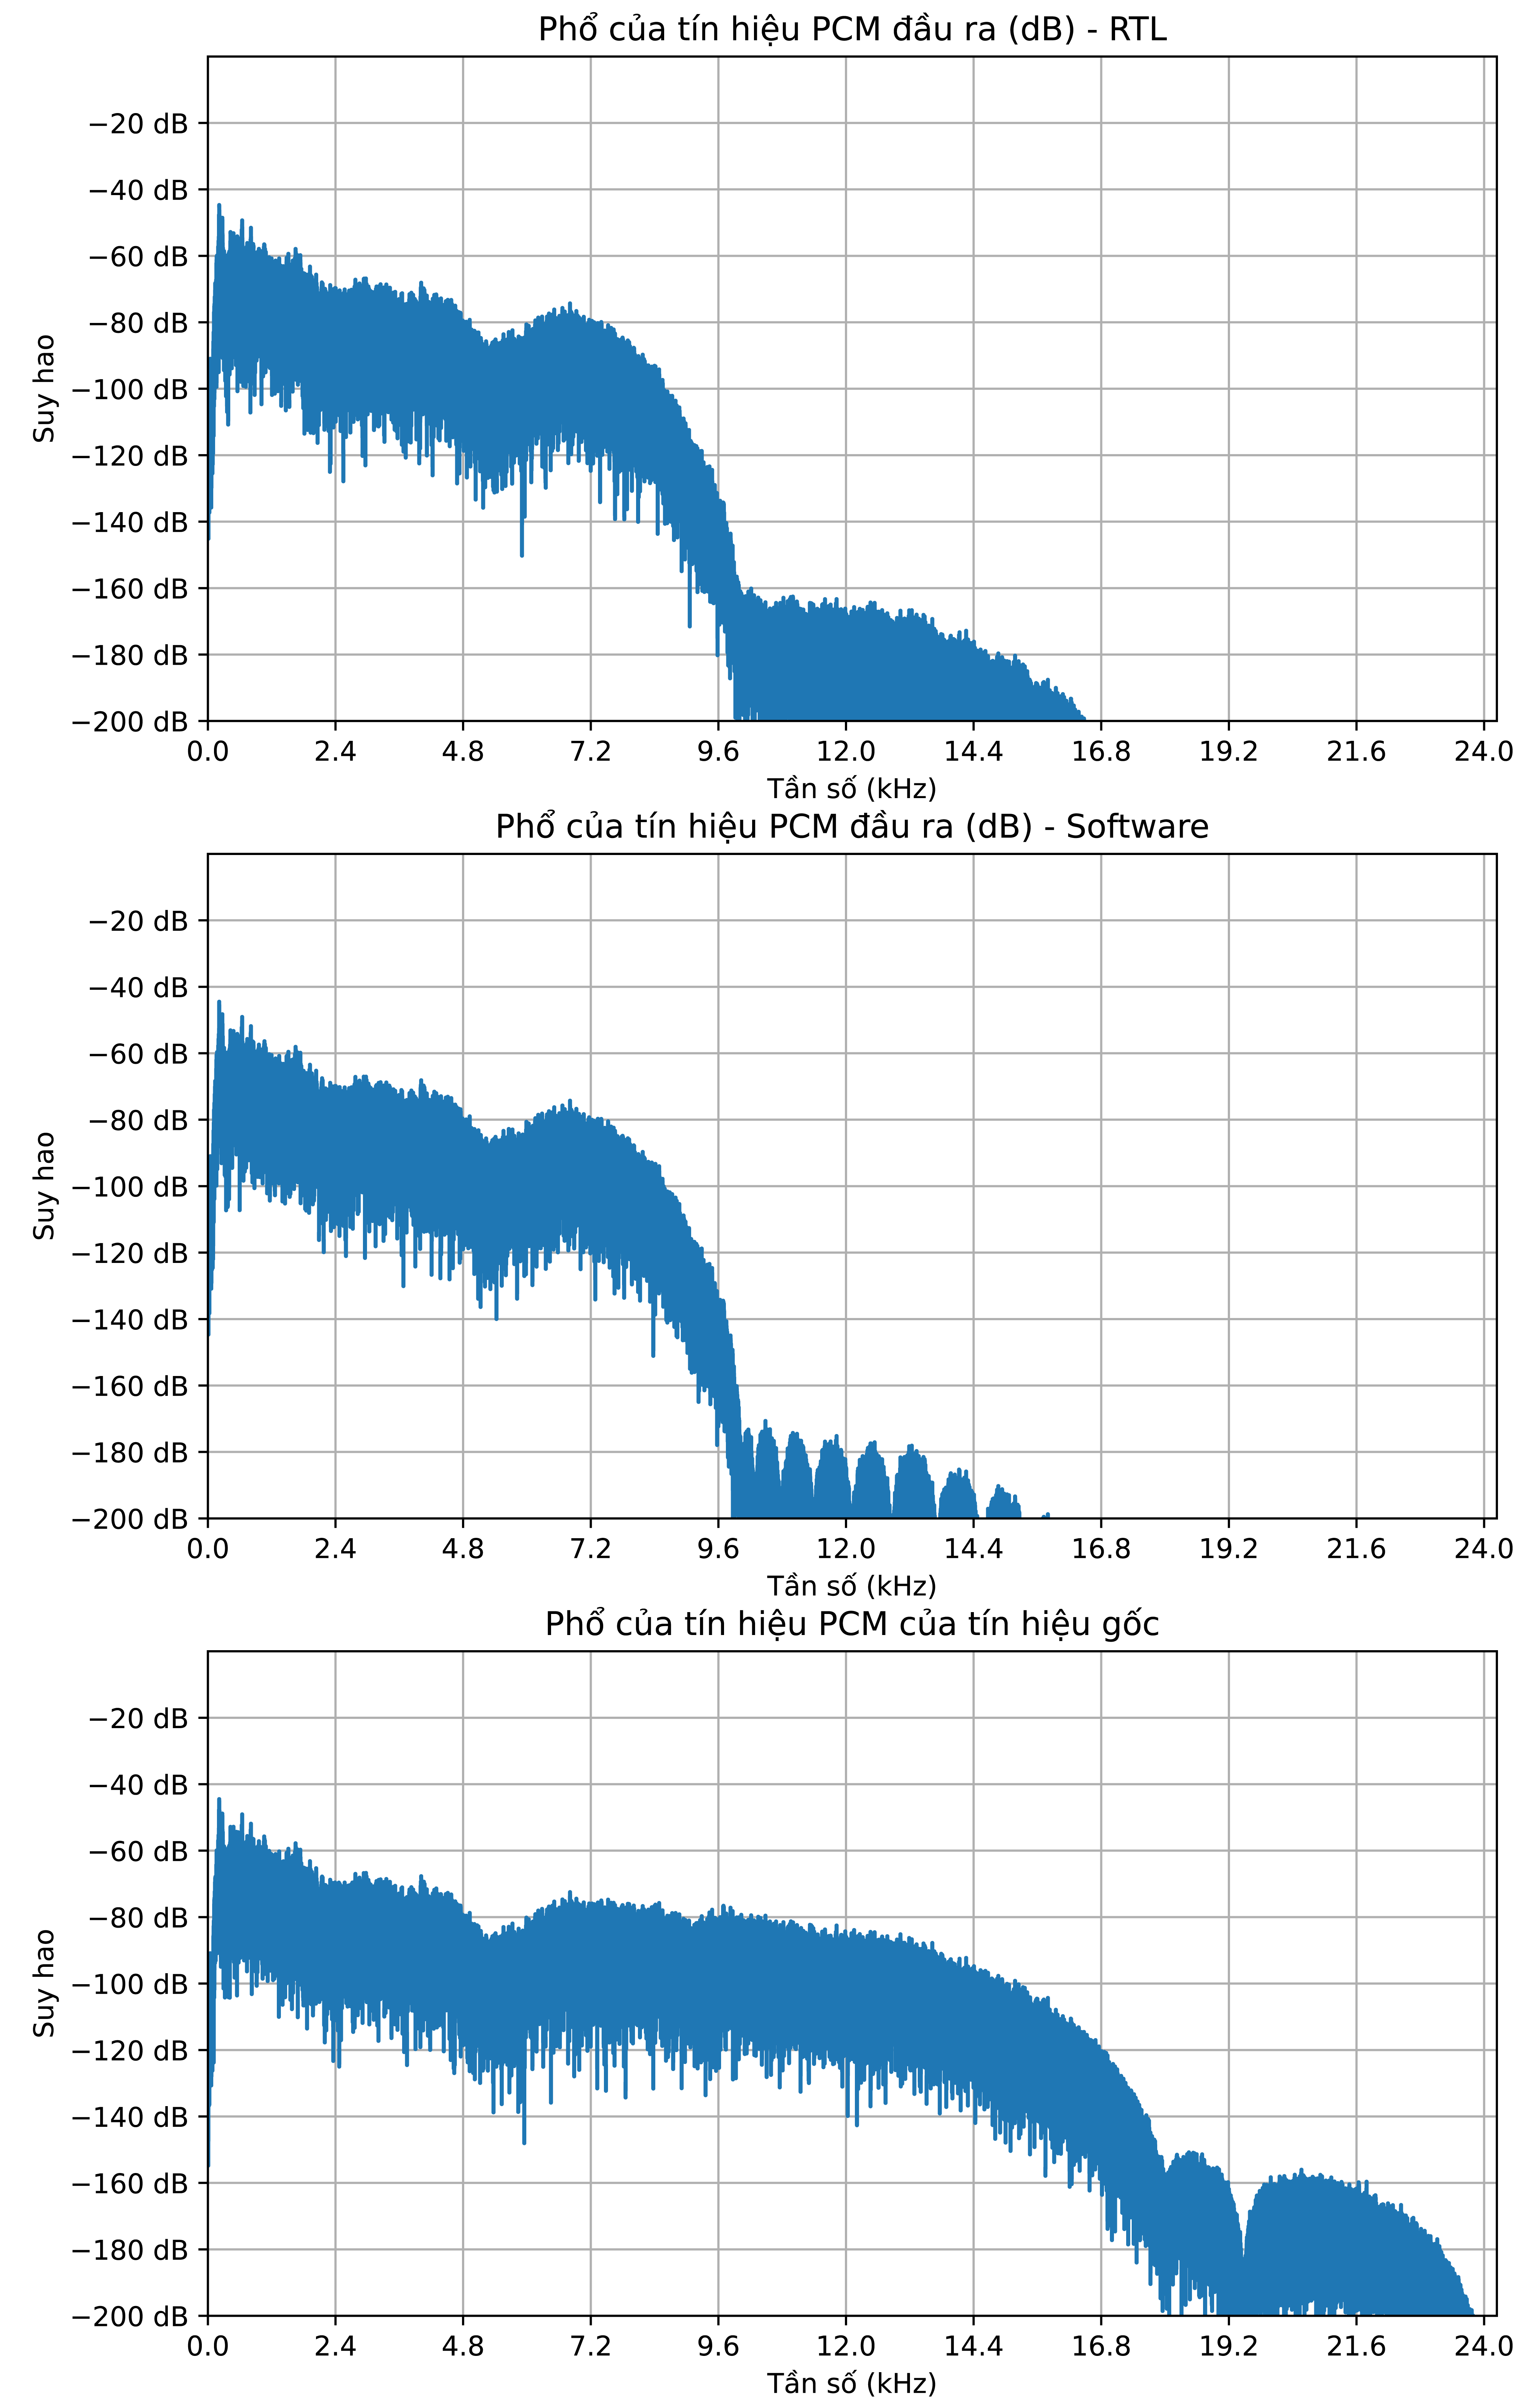
\includegraphics[width=13cm]{Images/Chuong4/tb/wav/vocal_psd.png}
    \caption[Biểu đồ phổ của âm thanh chỉ giọng nói trước và sau mô phỏng]{\bfseries \fontsize{12pt}{0pt}\selectfont  Biểu đồ phổ của âm thanh chỉ giọng nói trước và sau mô phỏng}
    \label{vocal_psd}
\end{figure}

Hình \ref{vocal} mô tả tín hiệu trước và sau chuyển đổi trên miền thời gian. Vì tín hiệu âm thanh giọng nói ở dải dừng có cường độ không cao nên sau khi xử lý không có sự khác biệt giữa gốc và sau mô phỏng.

\begin{figure}[H]
    \centering
    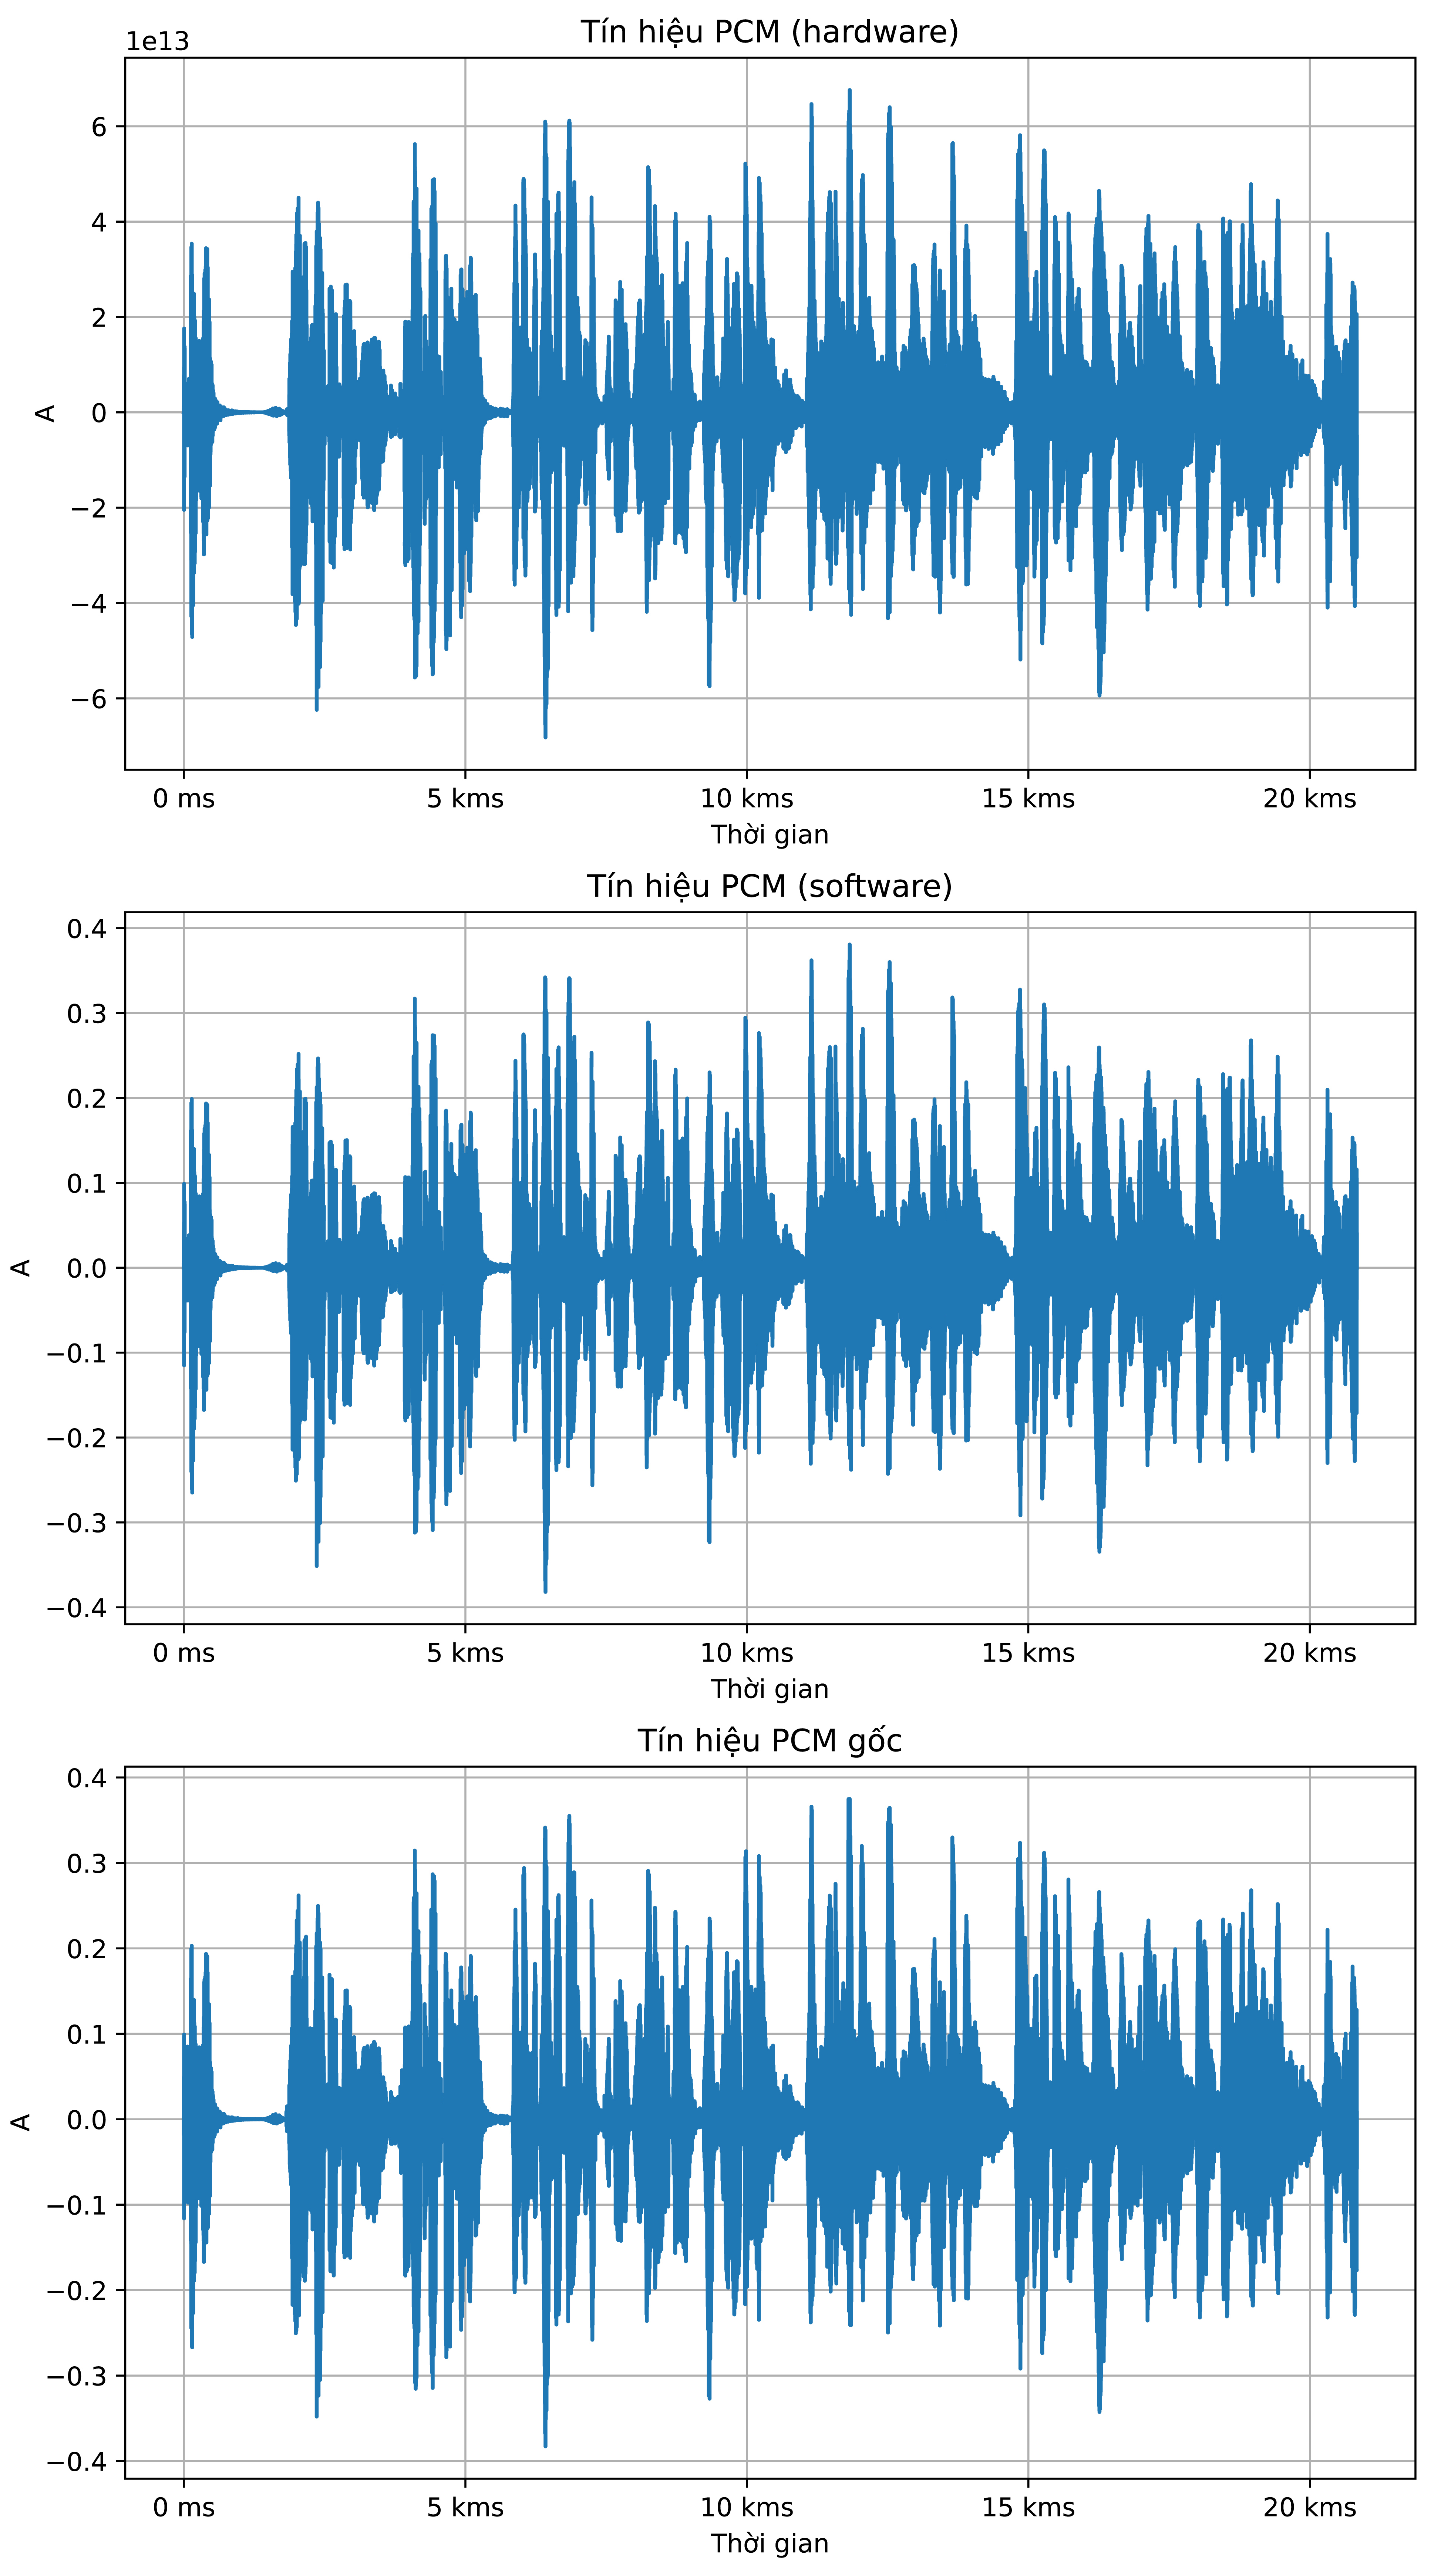
\includegraphics[width=12cm]{Images/Chuong4/tb/wav/vocal.png}
    \caption[Biểu đồ thời gian của âm thanh chỉ giọng nói trước và sau mô phỏng]{\bfseries \fontsize{12pt}{0pt}\selectfont Biểu đồ thời của âm thanh chỉ giọng nói trước và sau mô phỏng}
    \label{vocal}
\end{figure}



\subsection{Kết luận chương}

\hyperref[chuong4]{Chương 5} đã giải quyết được vấn đề thiết kế bộ chuyển đổi nhiều giai đoạn với ngôn ngữ mô tả phần cứng SystemVerilog. Kết quả kiểm thử cho thấy thiết kế có sai số so với việc tính toán bằng phần mềm nhưng vẫn đáp ứng được với các yêu cầu thiết kế đặt ra. Trong chương tiếp theo, thiết kế này sẽ được tổng hợp và triển khai lên FPGA để kiếm chứng tính đúng đắn trong điều kiện thực tế.

\newpage